% Options for packages loaded elsewhere
\PassOptionsToPackage{unicode}{hyperref}
\PassOptionsToPackage{hyphens}{url}
\PassOptionsToPackage{dvipsnames,svgnames,x11names}{xcolor}
%
\documentclass[
  letterpaper,
]{report}

\usepackage{amsmath,amssymb}
\usepackage{lmodern}
\usepackage{iftex}
\ifPDFTeX
  \usepackage[T1]{fontenc}
  \usepackage[utf8]{inputenc}
  \usepackage{textcomp} % provide euro and other symbols
\else % if luatex or xetex
  \usepackage{unicode-math}
  \defaultfontfeatures{Scale=MatchLowercase}
  \defaultfontfeatures[\rmfamily]{Ligatures=TeX,Scale=1}
\fi
% Use upquote if available, for straight quotes in verbatim environments
\IfFileExists{upquote.sty}{\usepackage{upquote}}{}
\IfFileExists{microtype.sty}{% use microtype if available
  \usepackage[]{microtype}
  \UseMicrotypeSet[protrusion]{basicmath} % disable protrusion for tt fonts
}{}
\makeatletter
\@ifundefined{KOMAClassName}{% if non-KOMA class
  \IfFileExists{parskip.sty}{%
    \usepackage{parskip}
  }{% else
    \setlength{\parindent}{0pt}
    \setlength{\parskip}{6pt plus 2pt minus 1pt}}
}{% if KOMA class
  \KOMAoptions{parskip=half}}
\makeatother
\usepackage{xcolor}
\usepackage[normalem]{ulem}
\setlength{\emergencystretch}{3em} % prevent overfull lines
\setcounter{secnumdepth}{5}
% Make \paragraph and \subparagraph free-standing
\ifx\paragraph\undefined\else
  \let\oldparagraph\paragraph
  \renewcommand{\paragraph}[1]{\oldparagraph{#1}\mbox{}}
\fi
\ifx\subparagraph\undefined\else
  \let\oldsubparagraph\subparagraph
  \renewcommand{\subparagraph}[1]{\oldsubparagraph{#1}\mbox{}}
\fi


\providecommand{\tightlist}{%
  \setlength{\itemsep}{0pt}\setlength{\parskip}{0pt}}\usepackage{longtable,booktabs,array}
\usepackage{calc} % for calculating minipage widths
% Correct order of tables after \paragraph or \subparagraph
\usepackage{etoolbox}
\makeatletter
\patchcmd\longtable{\par}{\if@noskipsec\mbox{}\fi\par}{}{}
\makeatother
% Allow footnotes in longtable head/foot
\IfFileExists{footnotehyper.sty}{\usepackage{footnotehyper}}{\usepackage{footnote}}
\makesavenoteenv{longtable}
\usepackage{graphicx}
\makeatletter
\def\maxwidth{\ifdim\Gin@nat@width>\linewidth\linewidth\else\Gin@nat@width\fi}
\def\maxheight{\ifdim\Gin@nat@height>\textheight\textheight\else\Gin@nat@height\fi}
\makeatother
% Scale images if necessary, so that they will not overflow the page
% margins by default, and it is still possible to overwrite the defaults
% using explicit options in \includegraphics[width, height, ...]{}
\setkeys{Gin}{width=\maxwidth,height=\maxheight,keepaspectratio}
% Set default figure placement to htbp
\makeatletter
\def\fps@figure{htbp}
\makeatother
\newlength{\cslhangindent}
\setlength{\cslhangindent}{1.5em}
\newlength{\csllabelwidth}
\setlength{\csllabelwidth}{3em}
\newlength{\cslentryspacingunit} % times entry-spacing
\setlength{\cslentryspacingunit}{\parskip}
\newenvironment{CSLReferences}[2] % #1 hanging-ident, #2 entry spacing
 {% don't indent paragraphs
  \setlength{\parindent}{0pt}
  % turn on hanging indent if param 1 is 1
  \ifodd #1
  \let\oldpar\par
  \def\par{\hangindent=\cslhangindent\oldpar}
  \fi
  % set entry spacing
  \setlength{\parskip}{#2\cslentryspacingunit}
 }%
 {}
\usepackage{calc}
\newcommand{\CSLBlock}[1]{#1\hfill\break}
\newcommand{\CSLLeftMargin}[1]{\parbox[t]{\csllabelwidth}{#1}}
\newcommand{\CSLRightInline}[1]{\parbox[t]{\linewidth - \csllabelwidth}{#1}\break}
\newcommand{\CSLIndent}[1]{\hspace{\cslhangindent}#1}

\usepackage{makeidx}
\makeindex
\makeatletter
\makeatother
\makeatletter
\@ifpackageloaded{bookmark}{}{\usepackage{bookmark}}
\makeatother
\makeatletter
\@ifpackageloaded{caption}{}{\usepackage{caption}}
\AtBeginDocument{%
\ifdefined\contentsname
  \renewcommand*\contentsname{Table of contents}
\else
  \newcommand\contentsname{Table of contents}
\fi
\ifdefined\listfigurename
  \renewcommand*\listfigurename{List of Figures}
\else
  \newcommand\listfigurename{List of Figures}
\fi
\ifdefined\listtablename
  \renewcommand*\listtablename{List of Tables}
\else
  \newcommand\listtablename{List of Tables}
\fi
\ifdefined\figurename
  \renewcommand*\figurename{Figure}
\else
  \newcommand\figurename{Figure}
\fi
\ifdefined\tablename
  \renewcommand*\tablename{Table}
\else
  \newcommand\tablename{Table}
\fi
}
\@ifpackageloaded{float}{}{\usepackage{float}}
\floatstyle{ruled}
\@ifundefined{c@chapter}{\newfloat{codelisting}{h}{lop}}{\newfloat{codelisting}{h}{lop}[chapter]}
\floatname{codelisting}{Listing}
\newcommand*\listoflistings{\listof{codelisting}{List of Listings}}
\makeatother
\makeatletter
\@ifpackageloaded{caption}{}{\usepackage{caption}}
\@ifpackageloaded{subcaption}{}{\usepackage{subcaption}}
\makeatother
\makeatletter
\@ifpackageloaded{tcolorbox}{}{\usepackage[many]{tcolorbox}}
\makeatother
\makeatletter
\@ifundefined{shadecolor}{\definecolor{shadecolor}{rgb}{.97, .97, .97}}
\makeatother
\makeatletter
\makeatother
\ifLuaTeX
  \usepackage{selnolig}  % disable illegal ligatures
\fi
\IfFileExists{bookmark.sty}{\usepackage{bookmark}}{\usepackage{hyperref}}
\IfFileExists{xurl.sty}{\usepackage{xurl}}{} % add URL line breaks if available
\urlstyle{same} % disable monospaced font for URLs
\hypersetup{
  pdftitle={Essays on Data Science},
  pdfauthor={Rafael C. Alvarado},
  colorlinks=true,
  linkcolor={blue},
  filecolor={Maroon},
  citecolor={Blue},
  urlcolor={Blue},
  pdfcreator={LaTeX via pandoc}}

\title{Essays on Data Science}
\author{Rafael C. Alvarado}
\date{9/20/23}

\begin{document}
\maketitle
\ifdefined\Shaded\renewenvironment{Shaded}{\begin{tcolorbox}[sharp corners, breakable, frame hidden, interior hidden, enhanced, borderline west={3pt}{0pt}{shadecolor}, boxrule=0pt]}{\end{tcolorbox}}\fi

\renewcommand*\contentsname{Table of contents}
{
\hypersetup{linkcolor=}
\setcounter{tocdepth}{2}
\tableofcontents
}
\bookmarksetup{startatroot}

\hypertarget{preface}{%
\chapter*{Preface}\label{preface}}
\addcontentsline{toc}{chapter}{Preface}

\markboth{Preface}{Preface}

\part{The History of Data Science}

\hypertarget{abstract}{%
\chapter{Abstract}\label{abstract}}

Consensus on the definition of data science remains low despite the
widespread establishment of academic programs in the field and continued
demand for data scientists in industry. Definitions range from rebranded
statistics to data-driven science to the science of data to simply the
application of machine learning to so-called big data to solve real
world problems. Current efforts to trace the history of the field in
order to clarify its definition, such as Donoho's ``50 Years of Data
Science'' (Donoho 2017), tend to focus on a short period when a small
group of statisticians adopted the term in an unsuccessful attempt to
rebrand their field in the face of the overshadowing effects of
computational statistics and data mining. Using textual evidence from
primary sources, this essay traces the history of the term to the early
1960s, when it was first used by the US Air Force in a surprisingly
similar way to its current usage, to 2012, the year that \emph{Harvard
Business Review} published the enormously influential article ``Data
Scientist: The Sexiest Job of the 21\textsuperscript{st} Century''
(Davenport and Patil 2012), even as the American Statistical Association
acknowledged a profound ``disconnect'' between statistics and data
science. Among the themes that emerge from this review are (1) a
continuous and consistent meaning of data science as the practice of
managing and processing scientific data from the 1960s to the present,
(2) a long-standing opposition between data analysts and data miners
that has animated the field since the 1980s, and (3) the phenomenon of
``data impedance''---the disproportion between surplus data, indexed by
phrases like ``data deluge'' and ``big data,'' and the limitations of
computational machinery and methods to process them. This persistent
condition appears to have motivated the use of the term and the field
itself since its beginnings.

\hypertarget{synopsis}{%
\chapter{Synopsis}\label{synopsis}}

Historically, there are two primary usages of ``data science'': the
classical and the statistical.

The classical usage began in the 1960s in the US military-industrial
sector and continues to this day in that area and in the data-driven
sciences. Among various public and private organizations that adopted
the term at that time, the Data Sciences Lab of the Air Force Cambridge
Research Laboratories formed in 1963 stands out (AFCRL 1963). This lab
established a paradigm that grew out of the need to dynamically process
vast amounts of sensor data---dubbed ``data deluge'' since the
1950s---in real-time to support decision-making and modeling of complex
phenomena. This lab pioneered the use of artificial intelligence and
computer visualization to extract patterns from new forms of data. Over
time this usage evolved to include working with large, complex, and
dynamic data sets in a variety of scientific fields, including physics,
environmental science, and biology.

A secondary development of the classical usage began in Silicon Valley
around 2008 and was famously promoted by \emph{Harvard Business Review}
in 2012 when it called data scientist the ``sexiest job of the 21st
century'' (Davenport and Patil 2012). In this usage, the paradigm of
classical data science jumped from the military-industrial and
scientific sectors to the commercial sector of so-called surveillance
capitalism (Zuboff 2019). In this context the usage became wildly
popular, prompting a high demand for data scientists in industry as well
as for authoritative explanations of the nature of the role. This in
turn motivated the formation of numerous degree programs throughout the
academy in the US, typically in the form of masters degrees. It also
elicited a strong reaction from academic statisticians alarmed by the
perceived disconnect between data science and their own field (Davidian
2013).

The statistical usage began in Japan in the early 1990s among academic
statisticians concerned with the threats and opportunities associated
with computational statistics, data mining, and other developments
relating to the rise of available computing and surplus data. Chikio
Hayashi coined this usage in 1992(Ohsumi 2002); by 1996 the
International Federation of Classification Societies (IFCS) adopted it
and began a long engagement with data science that continues to this day
in Europe and Japan(Hayashi 1998a). A parallel but shorter-lived version
of this usage emerged in the US between 1996 and 2001 when a small group
of academic statisticians unsuccessfully exhorted the field to brand
itself as data science and embrace new developments in computational
statistics and machine learning (Kettenring 1997b; C. F. J. Wu 1997;
Cleveland 2001). A third iteration of this usage was developed by
traditional statisticians who viewed the rise of second-wave classical
data science as a threat to their field that must be ``owned''(Rodriguez
2012; Davidian 2013; Yu 2014; {``ASA Statement on the Role of Statistics
in Data Science''} 2015; Donoho 2017).

The classical usage developed in the context of an historically unique
assemblage of networked data-generating and computational machinery that
characterized post-war military and scientific endeavors. The primary
problem faced in this context is what we can call data impedance---the
endemic disproportion between the production of data by
signal-generating instruments---from satellites and particle
accelerators to smart phones and credit cards---capturing a wide range
of natural and behavioral phenomena, and the ability to process and
interpret these data, often rapidly, by means of computational
machinery. In this context, data science emerged as an eclectic form of
expertise associated with the pipeline of activities that begins with
the acquisition of data, often from non-experimental sources, to its
reduction and modeling, to its visualization and interpretation.

By contrast, the statistical usage developed in the context of an
established academic field reacting to the very developments within
which classical data science emerged. Each iteration of this usage was
motivated by the perceived threats and opportunities opened by
computational methods and the growing surplus of data being captured by
databases and shared over networks. A recurrent theme in this usage is
an attraction to machine learning methods developed primarily by
computer scientists and a repulsion to data mining, perceived as an
unprincipled collection of methods lacking in experimental design and
mathematical grounding. In this context, data science emerged as a
rebranded form of statistics that would encompass and enhance the good
parts of the new computational methods while throwing away the bad.

\hypertarget{introduction}{%
\chapter{Introduction}\label{introduction}}

The interests of data scientists---the information and computer
scientists, database and software engineers and programmers,
disciplinary experts, curators and expert annotators, librarians,
archivists, and others, who are crucial to the successful management of
a digital data collection---lie in having their creativity and
intellectual contributions fully recognized.

National Science Board, ``Long-Lived Digital Collections: Enabling
Research and Education in the 21st Century'' (Simberloff et al. 2005:
27).

Data science today is characterized by a paradox. The large number and
rapid growth of job opportunities and academic programs associated with
the field over the past decade suggest that it has matured into an
established field with a recognizable body of knowledge. Yet consensus
on the definition of data science remains low. Members and observers of
the field possess widely variant understandings of data science,
resulting in divergent expectations of the knowledge, skill sets, and
abilities required by data scientists. Definitions, when they are not
laundry lists, range from a rebranded version of statistics to
data-driven science to the science of data to simply the application of
machine learning to so-called big data to solve real world problems.
These differences cannot be reduced to so-called semantics; they reflect
a range of deep-seated institutional commitments and values, as well as
variant understandings about the nature of knowledge and science. The
lack of shared understanding poses a significant problem for academic
programs in data science: it inhibits the development of standards and a
professional community, confounds the allocation of resources, and
threatens to undermine the authority and long-term prospects of these
programs.

This essay approaches the problem of defining data science by describing
how the collocation ``data science,'' and its grammatical variants
``data sciences'' and ``data scientist,'' have been used
historically.\footnote{In this essay, a collocation is defined as a
  combination of two or more words that function as a lexical unit. In
  contrast to a mere n-gram, its usage tends to be idiomatic and
  non-random. Etymologically, the usage of a collocation often begins as
  a marked construction, by means of quotes and hyphens, before
  eventually becoming idiomatic. Often, a collocation becomes so common
  that it becomes a single word. For example, the word ``database''
  began as ``data base'' and ``data-base'' before evolving into its
  current form (after beating out ``data bank''). Throughout this essay,
  the collocation ``data science'' is referred to as a term or phrase,
  reflecting its unitary semantic status.} The primary method employed
is the close reading and precise seriation of textual evidence drawn
from a representative collection of primary sources, including
organizational reports, academic articles, news stories, advertisements,
and other contemporary forms of evidence. These are used to trace the
history of the term's social and institutional contexts of use as well
as its denotative and connotative meanings. Extensive extracts are often
presented, rather than paraphrased, as these in many cases provide the
reader with direct and illuminating evidence for the meanings in
question.\footnote{The arguments and observations made by the authors in
  each case are represented in historical tense, not the textual
  present, which is the usual custom in writing about the history of
  ideas. For example, instead of saying that ``Tukey argues P'' in an
  essay from the 1960s, the evidence is presented as ``Tukey argued P.''
  This is done in order to ground the evidence in its social and
  historical setting.}

This historiography is presented as a series of decades in which the
term takes on a new meaning, beginning with its initial usage in the
1960s and ending around 2012, when the phrase becomes a commonplace. It
is shown that the phrase has a continuous and consistent usage
throughout this history. As usage of the phrase evolved, its meanings
were always additions to and inflections on prior meanings; in no case
did newer usages completely contradict what preceded them, nor did they
appear as cases of random independent invention.

The result is a picture of the transformation of a semantic complex that
indexes a consistent set of technical, social, and cultural realities
that constitute what may be called the situation of data science, a
situation that motivates the writing of this essay. Anticipating
follow-up research to this essay, this situation has been described
repeatedly by data scientists of all stripes as a kind of data
processing \emph{pipeline}, a sequence of operations that begins with
the consumption of data and ends with the production of data products,
ranging from research results and visualizations to software services
employed by various sectors of society.

\hypertarget{the-1960s}{%
\chapter{The 1960s}\label{the-1960s}}

\hypertarget{first-uses}{%
\section{First Uses}\label{first-uses}}

The first uses of the phrase ``data science,'' as a recognizable
collocation, appeared in the early 1960s in both singular and plural
forms. Two main uses are found in the written record almost
simultaneously, one in a military context, the other industrial. In both
cases, the phrase functioned as an organizational rubric for a new kind
of labor associated with the rise of large-scale data generating and
processing technologies that were the hallmark of the postwar era.

The military use first appeared in a series of reports covering the
period from July 1962 to June 1970 on research carried out by the Data
Sciences Laboratory (DSL). The DSL was founded in 1963 as one of several
labs associated with the US Air Force Cambridge Research Laboratories
(AFCRL).\footnote{The DSL was formed by combining the Computer and
  Mathematical Sciences Laboratory and the Communications Sciences
  Laboratory in the 1963 reorganization of the AFCRL (Venkateswaran
  1963: 628). Within the AFCRL, the lab was noted for its ``research on
  speech patterns {[}which{]} dated back to the 1940's {[}sic{]}''
  (Altshuler 2013: 27-28).} These reports do not provide an explicit
definition of data science or a rationale for choosing the expression
over others, but its meaning is clear from context. Consider the stated
motivation for the lab---which, as one of the first attested uses of the
phrase, is worth quoting at length:

\begin{quote}
The most striking common factor in the advances of the major
technologies during the past fifteen years {[}i.e.~since WWII{]} is the
increased use and exchange of information. \emph{Modern data processing
and computing machinery, together with improved communications}, has
made it possible to ask for, collect, process and use \emph{astronomical
amounts} of detailed data. \ldots{}

But in the face of this progress there is impatience with \emph{the
limitations of existing machines}. \ldots{}

A large number of military systems---for example, those concerned with
surveillance and warning, command and control, or weather
prediction---deal in \emph{highly perishable information}. Few existing
computers are capable of handling this information in
``real-time''---that is, processing the data as they come in. Higher
speed is one way to a solution. But increased speed will not overcome
fundamental shortcomings of existing computers. These shortcomings arise
from the fact that existing machines, having essentially evolved as
numerical calculators, are not always optimally organized to perform the
tasks they are called upon to do. \ldots{}

\ldots{} \emph{A considerable amount of the data to be processed is not
numerical}. It is in audio or visual form. Immense amounts of visual
data---for example, TIROS satellite pictures or bubble chamber pictures
of atomic processes---remain unevaluated for lack of processing
capability. In part this is due to the fact that, from the data
processing point of view, the information content of pictorial inputs is
highly redundant, \emph{demanding excessive channel capacity} in
transmission and compelling processing machinery to handle vast amounts
of meaningless or non-essential information. Similar considerations
prevail for speech. \ldots{}

In real-life situations \emph{data are almost never available in
unadulterated form}, but are usually distorted or masked by spurious
signals. Examples are seismic data, radio propagation measurements,
radar and infrared surveillance data and bioelectric signals. \ldots{}

An increasing amount of \emph{data processing research} is aimed at the
creation of machines or machine programs that incorporate features of
\emph{deductive and inductive reasoning, learning, adaptation,
hypothesis formation and recognition}. Such features are commonly
associated with human thought processes and, when incorporated in
machines, are frequently termed ``artificial intelligence.'' Artificial
intelligence is of utmost importance in decision situations where not
all possible future events can be foreseen {[}AFCRL (1963); emphasis
added{]}.
\end{quote}

The two later reports are more succinct:

\begin{quote}
The program of the Data Sciences Laboratory centers on the processing,
transmission, display and use of information. Implicit in this program
statement is an emphasis on computer technology (AFCRL 1967: 13).

Broadly defined, the program of the Data Sciences Laboratory involves
the automatic processing, filtering, interpretation and transmission of
information (AFCRL 1970: 318).
\end{quote}

Based on these excerpts alone, one could be forgiven for inferring that
data science was invented by the US Air Force around 1963 with the
formation of the DSL. Most of the elements currently considered central
to the field were brought together there: a concern for processing what
is later called ``big data,'' clearly defined in terms of volume,
velocity, and variety (and volatility); a recognition of the fundamental
messiness of data; and a focus on artificial intelligence as an
essential approach to extract value from such data. The lab produced
significant research on pattern recognition and classification, machine
learning, neural networks, and spoken language processing in the service
of processing the novel forms of data described above.

More important than locating a precise time and place for the origin of
the field---a task doomed to fail, given the complexity and
multithreaded nature of historical phenomena---is the work of describing
the historical situation within which the phrase data science developed
and which it indexes. A clue to this context is the repeated emphasis on
data and information processing we find in the DSL's descriptions of its
work. Specifically, the phrases ``the data processing point of view''
and ``data processing research'' index a set of military projects and
concerns associated with the early Cold War.

The AFCRL was originally established in 1945 as the Cambridge Field
Station, a unit created to hold onto the Harvard and MIT scientists and
engineers who performed significant research on radar and electronics in
WWII. During the 1950s, the lab focused on Project Lincoln, which led to
the creation of the Semi-Automatic Ground Environment (SAGE), a
real-time command-and-control system developed to counter to perceived
threat of an airborne nuclear attack by the Soviet Union. As a
continental air defense system, SAGE was designed to collect, analyze,
and relay data from a vast array of geographically distributed radars in
real-time, in order to initiate an effective response to an aerial
attack. At the heart of the system was a network of large digital
computers that coordinated the data retrieved from the radar sites over
phone lines and processed them to produce a single unified
image---literally displayed on a monitor---of the airspace over a wide
area.

Although responsibility for research on such military surveillance
systems was moved out of the lab in 1961, just before the Data Sciences
Lab was formed, it is plausible that the SAGE project influenced the
mission of the lab by providing a concrete paradigm for a new kind of
information processing situation. This was the situation of using of
advanced computational machinery and state-of-the-art data reduction and
pattern recognizing methods to process vast amounts of real-time signal
data, coming from geographically distributed radars and satellites, in
order to represent a complex space of operations and guide making
decisions about how to operate in that space. The paradigm was also
applied to the problem of weather forecasting and other geophysical
domains. (If we replace radars with smart phones and the Internet of
Things, it is not difficult to draw a parallel between this arrangement
and that of social media corporations today.)

Evidence for the influence of radar and satellite-based real-time
command and control systems on the conceptualization of data science may
be found in the idioms we currently associate with the field, such as
the use of ``signal and noise'' to refer to the presence and absence of
statistically significant patterns and the use of Receiver Operator
Characteristic (ROC) curves---first used by military radar operators in
1941---to measure the performance of binary classifiers. Other idioms,
such as ``data deluge,'' also emerge in this context. A history of the
expression data deluge is worth its own study, but it is clear that its
provenance was the situation described above. The term gained currency
in the 1960s in reference to satellite data collected by NASA and the
military. Consider this passage from the NASA publication
\emph{Scientific Satellites}:

\begin{quote}
The data deluge, information flood, or whatever you choose to call it,
is hard to measure in common terms. An Observatory-class satellite may
spew out more than 10\textsuperscript{11} data words during its
lifetime, the equivalent of several hundred thousand books. Data-rate
projections, summed for all scientific satellites, prophesy hundreds of
millions of words per day descending on Earth-based data processing
centers. These data must be translated to a common language, or at least
a language widely understood by computers (viz, PCM), then edited,
cataloged, indexed, archived, and made available to the scientific
community upon demand. Obviously, the vaunted information explosion is
not only confined to technical reports alone, but also to the data from
which they are written. In fact, the quantity of raw data generally
exceeds the length of the resulting paper by many orders of magnitude
(Corliss 1967: 157).\footnote{Preceding the usage of data deluge and in
  a wider context is ``information explosion.'' Both expressions conjure
  images of disaster and have been remarkably persistent up to the
  present era. Only with the coining of ``big data'' have they been
  displaced by a more positive term.}
\end{quote}

Work on such projects generated an enormous amount of research on the
problems arising from the processing and interpreting data. In the
preceding text, the author describes this work in some detail,
specifying a series of stages in which data are transformed into a form
suitable for scientific analysis. We would recognize this work today as
data wrangling. It is reasonable to infer that the concept of data
science emerged to designate this kind of work, which, in any case, is
consistent with the published mission of the Data Sciences Lab.

Prior to the formation of the DSL, the phrase ``data-processing
scientist'' was in use to designate the work involved in data reduction
centers, such as the one built at the Langley Aeronautical Lab in
Virginia to process the enormous amounts of data generated by wind
tunnel experiments and other sources associated with the nascent space
program. Data reduction was essential to projects like SAGE, in which
vast amounts of real-time signal data had to be reduced prior to
analysis. In a House appropriations hearing in 1958, the following
description of this kind of work was provided by Dr.~James H.
Doolittle,\footnote{This is the very same General Doolittle of
  Doolittle's Raid.} the last chairman of NACA before it became NASA:

\begin{quote}
The data processing function is much more complex than the mere
production line job of translating raw data into usable form. Each new
research project must be reviewed to determine how the data will be
obtained, what type and volume of calculations are required, and what
modifications must be made to the recording instruments and
data-processing apparatus to meet the requirements. \emph{It may even be
necessary for the data-processing scientist to design and construct new
equipment for a new type of problem.} Some projects cannot be undertaken
until the specific means of obtaining and handling the data have been
worked out. In some research areas, on-line service to a data processing
center saves considerable time by allowing the project engineer to
obtain a spot check on the computed results while the facility is in
operation. This permits him to make an immediate change in the test
conditions to obtain the results that he wants {[}U. S. C. H.
Appropriations (1958); emphases added{]}.
\end{quote}

\hypertarget{impedance}{%
\section{Impedance}\label{impedance}}

The kind of work conducted by NASA and the Air Force in this period
provides a context for understanding the meaning of data science when
the phrase first appeared. In this context, data science designated a
kind of research focused on what we may call the \emph{impedance} that
arises from the ever-growing requirements of data produced by an
expanding array of signal generating technologies (e.g.~radars and
satellites), scientific instruments, and reports on one hand, and the
limited capacity of computational machinery to process these on the
other. It is concerned specifically with the development of
computational methods and tools to handle the problems and harness the
opportunities posed by surplus data. In this context, \emph{data science
is the science of processing and extracting value from data by means of
computation}. Although the specific technologies have changed
continually, the condition of data impedance, the disproportion between
data abundance and computational scarcity relative to the need to
extract value from the data, has been constant since this time, and
defines the condition that gives rise to data science in this sense.

This interpretation of the meaning of data science is corroborated by
other contemporary usages. A report on a US Department of Defense
program to define standards ``to interchange data among independent data
systems'' refers to a ``Data Science Task Group'' established in 1966
``to formulate views of data and definitions of data terms that would
meet the needs of the program'' (Crawford, Jr. 1974: 51). Crawford, a
fellow student of Claude Shannon at MIT under Vannevar Bush, was
affiliated with IBM's Advanced Systems Development Division, a group
that had developed optical scanners to recognize handwritten numbers in
1964. In addition, the term appeared in the trademarked name of at least
two corporations in the United States: Data Science Corporation, formed
in 1962 by a former IBM employee ({``Robert Allen Obituary (2014) - St.
Louis, MO - St. Louis Post-Dispatch,''} n.d.), and Mohawk Data Sciences,
founded in 1964 by a three former UNIVAC engineers ({``Mohawk Data
Sciences''} 1966). Both companies provided data processing services and
lasted well into the era of personal computing. In the late 1960s and
1970s, many other companies used term as well, such as Data Science
Ventures (Mort Collins Ventures, n.d.) and Carroll Data Science
Corporation (Office 1979).\footnote{This continues into the 1980s, with
  Gateway Data Sciences Corp and Vertex Data Science, Ltd.}

\hypertarget{meaning-of-data-and-the-information-crisis}{%
\section{Meaning of ``data'' and the information
crisis}\label{meaning-of-data-and-the-information-crisis}}

Let us consider the meaning and significance of the word ``data'' in
these examples, especially given the DOD's concern to define it, as a
clue for the motivation of the term ``data science'' when other
candidates, such as computer science and information science, might have
sufficed at the time. The choice of the term appears to be motivated by
a concern to define and understand \emph{data} itself as an object of
study, a surprisingly opaque concept that is thrown into sharp relief in
the context of getting computers to do the hard work of processing
information in the context of impedance, as a result of their
commercialization and widespread use in science, industry, and
government. Thus although the term ``data'' has a long
history---deriving from the Latin word for that which is \emph{given} in
the epistemological sense, either through the senses, reason, or
authority---in this context it refers to the structured and discrete
representation of information sources so that these may be processed by
computers. In other words, \emph{data is machine readable
information}.\footnote{Preceding the usage of data deluge and in a wider
  context is ``information explosion.'' Both expressions conjure images
  of disaster and have been remarkably persistent up to the present era.
  Only with the coining of ``big data'' have they been displaced by a
  more positive term.} It follows that the data sciences in this period
are concerned with understanding machine readable information, in terms
of how to represent it and how to process it in order to extract value.

Further evidence of this concern for what might be called the
information crisis in scientific research---and for the idea that the
solution to this crisis hinges on refining the concept of data---can be
found in the formation of the International Council for Science (ICSU)
Committee on Data for Science and Technology (CODATA) in 1966. This
organization was established by an international group of physicists
alarmed that the ``deluge of data was swamping the traditional
publication and retrieval mechanisms,'' and that this posed ``a danger
that much of it would be lost to future generations'' (Lide and Wood
2012).~Importantly, CODATA still exists and currently identifies itself
with the field of data science. In 2001 it launched the \emph{Data
Science Journal,} focused on ``the management, dissemination, use and
reuse of research data and databases across all research domains,
including science, technology, the humanities and the arts'' ({``Data
Science Journal,''} n.d.). Aware that the definition of the field had
changed significantly since its founding, the journal provided the
following clarification in 2014:

\begin{quote}
We primarily want to \emph{specify} our definition of ``data science''
as the classic sense of the science of data practices that advance human
understanding and knowledge---the evidence-based study of the
socio-technical developments and transformations that affect science
policy; the conduct and methods of research; and the data systems,
standards, and~infrastructure that are integral to research.

We recognize the contemporary emphasis on data science, which is more
concerned with data analytics, statistics, and inference. We embrace
this new definition but seek papers that focus specifically on the data
concerns of an application in analytics, machine~learning, cybersecurity
or what have you. We continue to seek papers addressing data
stewardship, representation, re-use, policy, education etc.

Most importantly, we seek broad lessons on the science of data.
Contributors should generalize the significance of their contribution
and demonstrate how their work has wide significance or application
beyond their core study {[}Parsons (2019); emphasis in original{]}.
\end{quote}

This retrospective definition supports the idea that data science in the
1960s---which we may call, following this note, classical data
science---was concerned with understanding data practices, where data is
understood to be a universal medium into which information in a variety
of native forms, from scientific essays to radio signals from outer
space, must be encoded so that it may be shared and processed by
computational machinery. Data science as ``the science of data practices
that advance human understanding and knowledge'' is concerned with
defining and inventing this medium, its structure and function.

\hypertarget{a-note-on-tukey}{%
\section{A Note on Tukey}\label{a-note-on-tukey}}

Tukey's famous essay on data analysis, which appears during the same
time period, touches on some of the drivers noted here, such as the high
volume and spottiness of real data and the impact of the computer, but
from the perspective of advanced mathematical statistics (Tukey 1962).
One difference between his view and that adopted by the AFCRL is of
interest here: whereas Tukey appears to have regarded the computer as a
more or less fixed technology, replaceable in many tasks by ``pen,
paper, and slide rule'' but irreplaceable (he conceded) in others, the
Data Sciences Lab viewed the computer as a fluid technology, one that
needed to be pushed beyond its original design envelope as a numerical
calculator. In fact, the AFCRL and similar groups appear to have
provided the impetus to move computer science beyond a concern for
abstract algorithms and to include the study of data structures and
technologies, specifically databases. It is, as we shall see, a
difference that continues to underlie current disputes over the meaning
and value of data science.

\hypertarget{the-1970s}{%
\section{The 1970s}\label{the-1970s}}

\hypertarget{data-science}{%
\subsection{Data Science \ldots{}}\label{data-science}}

It is clear that by the early 1970s the term data science had been in
circulation in several contexts and referred to ideas and tools relating
to computational data processing. Importantly, these usages were not
obscure---the AFCRL was one of the premier research laboratories in the
world and closely connected with Harvard and MIT (Altshuler 2013), an
international cross-roads of intellectual life where many would have
come into contact with the term. Similarly, IBM and UNIVAC, the sources
of the founders of two self-proclaimed data science companies, were the
two largest computer manufacturers at the time.\footnote{As evidence for
  the visibility of the AFCRL as this time, here is an add that appeared
  in a 1964 issue of the British weekly \emph{Nature}:

  A SYMPOSIUM on ``Models for the Perception of Speech and Visual
  Form'', sponsored by the Data Sciences Laboratory of the Air Force
  Cambridge Research Laboratory, will be held in Boston during November
  11-14. Further information can be obtained from Mr.~G. A. Cushman,
  Wentworth Institute, 550 Huntington Avenue, Boston, Massachusetts
  02115 ({``Announcements''} 1964).}

\hypertarget{naurs-datalogi}{%
\subsection{\texorpdfstring{Naur's
\emph{Datalogi}}{Naur's Datalogi}}\label{naurs-datalogi}}

Although the AFCRL closed the Data Sciences Lab by 1970,\footnote{Altshuler
  writes that the lab was ``abolished'' in June 1972 ``in response to a
  large reduction in manpower authorizations'' (Altshuler 2013: 27).
  However, the unit is not mentioned in the July 1970 to June 1972
  research report (AFCRL 1973). The lab's closure may have been a
  consequence of the passing of the Mansfield Amendment in 1969, which
  prohibited the military from carrying out ``any research project or
  study unless such project or study has a direct and apparent
  relationship to a specific military function'' (U. S. C. H. C. on
  Appropriations 1970: 348).} the term continued to be used, most
notably by the Danish computer scientist Peter Naur, who suggested that
computer science, a relatively new field, be renamed to data science.
His argument, consistent with previous usage, was that computer science
is fundamentally concerned with data processing and not mere
computation, i.e.~what the AFCRL derided as numerical calculation.
Earlier, in the 1960s, Naur had coined the term ``datalogy'' (Danish:
\emph{datalogi}) for this purpose, but later found the term data science
to be a suitable synonym, perhaps due to its currency or to his
familiarity with the DSL, which shared his research interest in
developing programming languages (Naur 1966, 1968). In contrast to the
AFCRL, Naur provided an explicit definition of data science:

\begin{quote}
The starting point is the concept of \emph{data}, as defined in
{[}0.7{]}: DATA: \emph{A representation of facts or ideas in a
formalized manner capable of being communicated or manipulated by some
process.} Data science is the science of dealing with data, once they
have been established, while the relation of data to what they represent
is delegated to other fields and sciences.

The usefulness of data and data processes derives from their application
in building and handling models of reality.

\ldots{}

A basic principle of data science is this: The data representation must
be chosen with due regard to the transformation to be achieved and the
data processing tools available. This stresses the importance of concern
for the characteristics of the data processing tools.

Limits on what may be achieved by data processing may arise both from
the difficulty of establishing data that represent a field of interest
in a relevant manner, and from the difficulty of formulating the data
processing needed. Some of the difficulty of understanding these limits
is caused by the ease with which certain data processing tasks are
performed by humans {[}Naur (1974): 30-31; emphasis and citation in
original; the reference ``0.7'' refers to Gould (1971){]}.
\end{quote}

Clearly, Naur's definition inherits the classical definition described
above; it locates the meaning of the term in the series of practices
associated with the larger activity of data processing. These practices
include establishment, choice of representation, conversion and
transformation, the modeling of reality, and the guiding of human
actions. One difference is that Naur is keen to locate data science
within a division of labor implied by this general process, separating
data science \emph{per se} from the work of data acquisition
(establishment) and the domain knowledge required to acquire data
effectively. In this view, data science is more specifically concerned
with the formal representation of data (i.e.~with data structures and
models), a practice that must be done in light of how data are to be
transformed downstream, and with which tools (i.e.~algorithms and
programming languages). As we shall see, the weighting that Naur assigns
to this kind of work is not inherited by later theorists. However, the
general image of a sequential process with distinct phases in the life
cycle of data is. Here we see the appearance of the image of a pipeline,
unnamed but implied by the concept of \emph{process}, which dominates
the mental representation of the field from its origins in the 1960s.

Far from being a fluke, Naur's usage developed the classical definition
of data science initiated by NASA and the Air Force, intentionally or
not. The fact that his attempt to rename computer science failed outside
of his native country (and Sweden) is not important; his understanding
of computer science sheds light on how closely the concept of data was
(and is) related to computation and process.

It is worth noting that Naur's definition implies a familiarity with the
real-world provenance of data processing in industry and government.
Indeed, by this time computational data processing had penetrated all
sectors of society, and the pressure to improve tools and methods to
represent and process data had increased as well. As a result of this
pressure, two important data standards were developed in this period:
Codd's relational model, which laid the foundation for SQL and
commercially viable relational databases in the 1980s, and Goldfarb's
SGML, which would become a standard for encoding so-called unstructured
textual data (such as legal documents) and later the basis for HTML and
XML Goldfarb (1970). This focus on the human context of data processing
is reflected in his later work; a volume of selections of his writing
from 1951 to 1990, which includes his essay on data science, is entitled
``Computing: A Human Activity'' (Naur 1992).

\hypertarget{other-uses}{%
\subsection{Other Uses}\label{other-uses}}

\begin{itemize}
\item
  (\emph{Computers in Education: Proceedings of the IFIP ... World
  Conference} 1975) Computers in Education, Proceedings of the IFIP
  World Conference

  \begin{itemize}
  \item
    ``The case is easily obscured, alas, by an instinct to confuse
    mathematics and data science'' (p.~756)
  \item
    ``Recommending data science and data technology as areas of
    intellectual endeavor, and data studies as a subject for school
    learning;'' (p.~758)
  \end{itemize}
\end{itemize}

\hypertarget{the-1980s}{%
\section{The 1980s}\label{the-1980s}}

\hypertarget{the-1990s-statistical-data-science}{%
\chapter{The 1990s: Statistical Data
Science}\label{the-1990s-statistical-data-science}}

Interestingly, in 1977 a prefixed variant of the term appeared in the
title of the technical report, ``Non-Parametric Statistical Data
Science: A Unified Approach Based on Density Estimation and Testing for
`White Noise'\,'' (Parzen 1977). However, Parzen later published a
version of this work as ``Nonparametric Statistical Data Modeling''
(Parzen 1979), which indicates that his original word choice was
mistaken. Yet the original choice may not have been entirely
unmotivated: Parzen's work attempted to unify parametric and
non-parametric methods under one umbrella. Given the natural inclination
of mathematical statistics for the former and data analysis for the
latter, his choice of the term data science may have signaled an attempt
to encompass both approaches to data. It is also worth noting that he
later used to the term to introduce a ``new culture of statistical
science called LP MIXED DATA SCIENCE'' (Parzen and Mukhopadhyay 2013),
after the term became popular.\footnote{Parzen's use of the term
  ``culture'' here echoes his comments on Breiman's famous essay on two
  cultures of statistical models, where he suggested that there are in
  fact several cultures, including his own, to which he devoted the
  majority of his response (Breiman 2001: 224--226).} Whether or not
this unifying goal was his motivation, statisticians later became quite
interested in the term for precisely this reason.

\hypertarget{the-tokyo-school}{%
\section{1994: The Tokyo School}\label{the-tokyo-school}}

\hypertarget{ohsumi-and-meta-stat}{%
\subsection{Ohsumi and Meta-Stat}\label{ohsumi-and-meta-stat}}

In the early 1990s, the term resurfaced in the context of statistics. It
appeared in the title of a 1994 essay by the Japanese statistician
Noburu Ohsumi on the application of hypermedia to the problem of
organizing data, ``New Data and New Tools: A Hypermedia Environment for
Navigating Statistical Knowledge in Data Science,'' an elaboration of an
essay published two years earlier (Ohsumi 1992, 1994).\footnote{According
  to Ohsumi, ``the term `data science' appeared for the first time'' in
  1992, at a research exchange meeting between French and Japanese data
  analysts (so-called) at Montpelier University II in France (Ohsumi
  2000: 331). He also claims to have ``argued the urgency of the need to
  grasp the concept `data science'\,'' in 1992 (329).} In these essays,
Ohsumi described the by now familiar litany of problems associated with
data impedance, although this time the focus was on the production of
data resulting from its analysis and storage, not its consumption in
so-called raw form:

\begin{quote}
In research organizations handling statistical information, the volume
of stored information resources, including research results, materials,
and software, is increasing to the point that conventional separate
databases and information management systems have become insufficient to
deal with the amount. Increasing diversification in the media used these
days interferes with the rapid retrieval and use of the information
needed by users. A new system that realizes a presentation environment
based on new concepts is needed to inform potential users of the value
and effectiveness of using the vast amount of diverse data (Ohsumi 1992:
375).
\end{quote}

For research facilities around the world, the products of classical data
science---the database and data processing software---had become a
sorcerer's apprentice, creating new problems with each solution.
Organizations were drowning in the data sets they produced or acquired,
the software used to process them, the print and digital libraries of
reports and articles resulting from their analyses, and a host of other
materials. The requirements, approach, and design goals of Ohsumi's
proposed system, the Meta-Stat Navigator, are strikingly similar to
those of a contemporary system designed to solve the information
problems of another scientific organization: Berners-Lee's World Wide
Web, famously developed at CERN in 1989 (Berners-Lee and Fischetti
2008). Of course, the latter quickly obviated Ohsumi's proposal and
become synonymous with the Internet, invented decades earlier.

The significance of Meta-Stat for our purposes is that this kind of work
was understood clearly as data science at this point in history. Data
science continued to be connected with the processing and representation
of data, and was distinct from data analysis, but with this important
development: statisticians had become embedded in these technologies,
and their work had changed significantly as a result. And, as a result
of this change in working conditions, the connection between data
analysis and data science became closer.

Here we may locate with some precision a crucial transformation in the
meaning of the term, associated with its adoption by a new set of users.
One clue to this change is the opportunity Ohsumi observed amid the
challenges posed by data deluge:

\begin{quote}
\ldots{} the information handled by the statistical sciences lies on the
boundaries of various other sciences and clarifies the relationships and
nature of information that joins these sciences. Development of a system
that fully organizes and integrates strategic information is essential
(Ohsumi 1992: 375).
\end{quote}

The Meta-Stat ``system'' was designed to realize the opportunity opened
up by the central position statisticians had come to occupy among the
prolifically data-generating sciences and the computational environment
in which these data were made available. Data science, in this view, is
\emph{meta-statistics}, an encompassing concern for understanding data,
understood as a universal medium, and its relationship to knowledge.

This perspective was shared by Ohsumi's senior compatriot and fellow
statistician, Chikio Hayashi, whom Ohsumi described as ``the pioneer and
founder of data science'' (Ohsumi 2004: 1).\footnote{In his eulogy for
  Professor Hayashi, Ohsumi explained in some detail the motivation for
  his mentor's first usage of data science:

  \begin{quote}
  In the last ten years of his life, Professor Hayashi asserted the
  importance of ``data science as a theory of scientific methods.'' The
  starting point was the meaning of the words ``data science;'' this
  arose in 1992, when the professor was discussing the titles and
  introductions of a collection of papers to be published at the 2nd
  Japanese-French Scientific Seminar. \emph{The professor used a
  Japanese phrase that translates as ``data science'' and for the rest
  of his life explored the concept behind this phrase.} When the papers
  at the seminar were published, it was proposed for the first time that
  the term referring to quantification be standardized as
  ``quantification method'' and the subsequent English terms were
  standardized as such. I can recall the professor reprimanding us with
  the words ``you are talking about different concepts'' when we
  referred to ``deta kagaku'' while another group called it ``deta no
  kagaku'' (data science).

  The basis of data science is an extremely straightforward concept; the
  fact that it needed to be expressed is an indication of the chaos that
  exists today in statistical data analysis and the deteriorating
  research environment. I am certain that the professor had intended to
  lead the way in achieving a breakthrough on these problems {[}Ohsumi
  (2002): 5; emphasis added{]}.
  \end{quote}

  \hypertarget{section}{%
  \subsubsection{}\label{section}}}

\hypertarget{hayashis-usage}{%
\subsection{Hayashi's Usage}\label{hayashis-usage}}

\hypertarget{section-1}{%
\subsubsection{1993}\label{section-1}}

In 1993, at a round table discussion during the fourth conference of the
International Federation of Classification Societies held in Paris
(IFCS-93), Hayashi uttered the phrase ``Data Science'' and was then
asked to explain it. At the next conference (IFCS-96), he presented an
answer, in addition to having the conference named to emphasize the
importance of the term---``Data Science, Classification, and Related
Methods.'' His definition is as follows:

\begin{quote}
Data science is not only a synthetic concept to unify {[}mathematical{]}
statistics, data analysis and their related methods but also comprises
their results. It includes three phases, design for data, collection of
data, and analysis on data. Data science intends to analyze and
understand actual phenomena with ``data.'' In other words, the aim of
data science is to reveal the features of the hidden structure of
complicated natural, human and social phenomena with data from a
different point of view from the established or traditional theory and
method. This point of view implies multidimensional, dynamic and
flexible ways of thinking (Hayashi 1998b: 41).
\end{quote}

Hayashi went on to describe the sequence of design, collection, and
analysis as a primary and iterative ``structure finding'' process in
which data are transformed from a state of ``diversification,'' given
the inherent ``multifariousness'' of the phenomena they represent, to
one of ``conceptualization or simplification'' (41). The discovery of
structure is accomplished with what we would recognize today as the
methods of exploratory data analysis and unsupervised learning. In
effect, Hayashi's definition abstracted the design goals of Ohsumi's
Meta-Stat system and presented them as ``a new paradigm'' of science,
one that would encompass statistics, data analysis, and their vast
output of data within in a unified, process-oriented framework---data
science (40).

In addition to Hayashi's own definition, it helpful also to see how the
field was defined by the editors (who included Hayashi) of the
proceedings of IFCS-96:

\begin{quote}
The volume covers a wide range of topics and perspectives in \emph{the
growing field of data science}, including theoretical and methodological
advances in domains relating to data gathering, classification and
clustering, exploratory and multivariate data analysis, and knowledge
discovery and seeking.

It gives a broad view of the state of the art and is intended for those
in the scientific community who either develop new data analysis methods
or gather data and use search tools for analyzing and interpreting large
and complex data sets. Presenting a wide field of applications, this
book is of interest not only to data analysts, mathematicians, and
statisticians but also to scientists from many areas and disciplines
concerned with complex data: medicine, biology, space science,
geoscience, environmental science, information science, image and
pattern analysis, economics, statistics, social sciences, psychology,
cognitive science, behavioral science, marketing and survey research,
data mining, and knowledge organization {[}Hayashi (1998a): v; emphasis
added{]}.
\end{quote}

Of interest here is use of ``data science'' as a big tent, an inclusive
rubric under which to group a series of domains (which match roughly to
a process) as well as a broad range of disciplines and levels, from tool
builders to scientists and practice to theory. This passage is also
significant for including within the scope of data science the methods
of machine learning as well as data mining among the list of sciences
concerned with ``complex data,'' suggesting the prominence of these
approaches at that time. We will see that not all definitions proceeding
from this community were as inclusive.

Hayashi assigned a revolutionary and almost messianic role to data
science. In his vision, the statistical sciences had lost their way.
Mathematical statisticians had come to overvalue abstract inference and
precision, and by choosing to work with the artificial data required to
pursue these goals were ``prone to be removed from reality'' (40). Data
analysts, although working with real data, had ``come to manipulate or
handle only existing data without taking into consideration both the
quality of data and the meaning of data \ldots{} to make efforts only
for the refinement of convenient and serviceable computer software and
to imitate popular ideas of mathematical statistics without considering
the essential meaning'' (40). As a result of these divergent attitudes
toward data, and the disregard of both for the scientist's engagement
with the primary, existential relationship between data and phenomena,
the field had become stagnant and lacking in innovation. Data science
emerged as a savior, unifying a divided people, showing their way out of
the wilderness, and restoring prosperity and prestige to their
community.

If Hayashi's criticisms of data analysis sound familiar to those leveled
today against data scientists, it is because the issues data science was
meant to resolve are recurring and systemic. So too is the separation
between data analysis and mathematical statistics, which was recognized
by Box, and later Tukey, in the 1970s. In his response to Parzen---who,
we noted, sought to overcome a methodological split between the two
subfields---Tukey wrote:

\begin{quote}
I concur with the general sentiments expressed by George Box in his
Presidential Address \ldots{} that we have great need for the whole
statistician in one body---for the analyst of data as well as for the
probability model maker---and the inferential theorist/practitioner. One
cannot, however, make a whole man by claiming that one can subsume one
important class of mental activity under another class whose style and
purposes are not only different but incompatible. To be ``whole
statisticians'' as Box might put it, or to be ``whole statistician-data
analysts'' as I might, means to be single persons who can take quite
different views and adopt quite different styles as the needs change. As
the title of my paper of yesterday put it, ``we need both exploratory
and confirmatory''! The twain can---and should---meet, but they need to
remain a pair (or two distinct parts of a larger team) if they are to do
what they should and can (Tukey 1979: 122).
\end{quote}

Tukey implies a solution to the schism, later observed by Hayashi, in
better organization, not in a utopian ``new man'' or in a synthetic
science \emph{per se}, recalling the division of labor proposed by Naur,
but here focusing on different roles within that division. Implicit in
this approach is the view that the problem with statistics was not
epistemic but organizational.

Here it is helpful to recall a property of Kuhn's concept of
paradigm---an obvious lens through which to observe our topic---which is
often overlooked by those who use the term: it refers no to an abstract
body of ideas that succeed on the basis of their intrinsic rationality
or truth value, but to the successful practical application of ideas by
means of novel methods and tools in a way that they may be imitated. The
concept has both epistemic and social dimensions. Viewed in this light,
the question of whether data science is in fact a science---our main
question---becomes a matter of determining whether it solves important
problems in new ways, by means of an assemblage of ideas, methods, and
tools that may be grasped and imitated by others. Hence, although Tukey
and Hayashi may appear to be divergent in their approaches to overcoming
the problems, they represent the two aspects of a scientific paradigm,
the one conceptual, the other practical. This should not be viewed as
contradictory.

\hypertarget{a-canary-the-has-forgotten-to-sing}{%
\subsection{A Canary the has Forgotten to
Sing}\label{a-canary-the-has-forgotten-to-sing}}

Following the IFCS meetings, as well as two meetings of the Japan
Statistical Society that held ``special sessions on data science,'\,'
Ohsumi developed Hayashi's definition as well as its rationale (Ohsumi
2000: 331). We call this the Tokyo school of data science, given the
association of both Hayashi and Ohsumi with the Institute of Statistical
Mathematics in Tokyo, Japan. In a paper that explicitly addressed the
relationship between data analysis and data science, and which is
perhaps the first of several to claim the flag of data science for
statistics, Ohsumi declared that because of its privileging
of''mathematical methodologies'' over an engagement with data
acquisition, data analysis had become ``a canary that has forgotten to
sing,'' referring to a Japanese children's song that contemplates a
silent bird's fate (332).\footnote{The specific reference is to a poem,
  later set to music, written by the Japanese poet Saijoo Yaso
  (西条八十), who lived from 1892 to 1970. According to Miriam Davis,
  ``The moral of the song is that if the canary loses its song it is not
  worth its existence so it should make the most of the gift of song it
  has been given.'' (Davis, n.d.)} Amplifying Hayashi, he asserted that
``{[}h{]}ow data are gathered is the key to defining the relevant
information and making it easy to understand and analyze'' (331). In
making this point, Ohsumi referred to a new figure on the scene, one
that contradicted the principles he proposed:

\begin{quote}
In my opinion, this viewpoint on the meaning of data science is
fundamentally different from data mining (DM) and knowledge discovery
(KD). These concepts are not of practical use because they neglect the
problems of ``data acquisition'' and its practice (332).
\end{quote}

It is significant that Ohsumi excludes these new fields---or field,
since the two so frequently co-occur, along with the variant KDD,
``knowledge discovery in databases''---from his definition of data
science, since many today would consider the two synonymous.

\hypertarget{data-mining-and-knowledge-discovery}{%
\section{Data Mining and Knowledge
Discovery}\label{data-mining-and-knowledge-discovery}}

The paradox is instructive: the name ``data mining,'' as used here, made
its appearance in the late 1980s and early 1990s as a rubric that
included a set of practices motivated by precisely the same conditions
that led the Tokyo school to propose the field of data science in the
first place. Among these conditions was the relatively sudden appearance
of vast amounts of data stored in databases---one of the fruits of
classical data science---owing to the rise of relational databases and
personal computing in the 1980s, and a suite of tools to work with data,
from spreadsheets to programming languages to statistical software
packages. Whereas many statisticians viewed these developments with
alarm, being acutely aware of the epistemic disruptions they produced
for the received workflow of data analysis, the data mining community
embraced them as an opportunity to convert data into value. Coming
mainly from the field of computer science, data miners developed a set
of methods that included the application of machine learning algorithms
to the data found in databases in various contexts, from science to
industry (such as point-of-sale records generated as by-product of
computerized cash registers and credit card use). The relationship
between machine learning and data mining was also mutually
beneficial---data miners supplied machine learning projects with the
large sets of data required for this class of algorithms to perform
well. This relationship was greatly reinforced with the rise and
development of the Web and social media platforms, which generated
enormous amounts of behavioral data.

Although the two fields---for simplicity, let's call them data analysis
and data mining---were responding to the same conditions of data surplus
and impedance, their philosophical orientations could not have been more
opposed. This difference is clearest in their respective evaluations of
data \emph{provenance}, the source and conditions under which data are
produced. For the data miner, data provenance is largely irrelevant to
the possibility of converting data into value. Data are data, regardless
of how they are generated, and the same methods may be applied to them
regardless of source, so long as their structure is understood. Indeed,
for the data miner data exists much as natural resources do, as a given
part of the environment, which helps explain the success of the metaphor
of \emph{mining} over competing variants, such as \emph{harvesting},
which implies intentional creation. For the data analyst, as Hayashi and
Ohsumi took such pains to emphasize, provenance is, or should be,
everything, echoing the statistician's orthodox preference for
experimental over observational data.

This difference was expressed by Ohsumi in his definition of data
science in opposition to data mining:

\begin{quote}
Owing to the qualitative and quantitative changes in data {[}produced by
the conditions described above{]}, it is, indeed, becoming increasingly
difficulty to grasp all aspects of a dataset in explaining various
phenomena. Therefore, new techniques, such as DM, KD, complexity, and
neural networks, are being proposed. However, the potential of these
methods to solve any of these problems is questionable (332).
\end{quote}

Ohsumi went on to characterize the way data has changed by listing the
new kinds of data with which the statistician is confronted. These
include prominently data sets found in databases as by-products of
various processes, such as passive accumulation (e.g.~from point-of-sale
devices), unstructured data (included in text fields), and aggregated
data generated ``spontaneously and accumulating automatically in the
electronic data collection environment'' (332-333). He explained his
concern with data mining:

\begin{quote}
When it comes to analyzing these datasets, people discuss DM and related
techniques. However, the important questions to answer are: what dataset
is necessary to explicate a certain phenomenon, why is it necessary, how
to design its acquisition, and how difficult the whole process is.
\emph{This is more important than the dataset itself}. Books on DM do
contain terms such as ``data preparation'', ``getting the data'',
``sampling procedures'', and ``data auditing'', but there is an
assumption that the dataset is given and the procedure may start with
analysis. Fiddling with a dataset once it is collected is merely a
self-contained play of data handling {[}Ohsumi (2000): 333; emphasis
added{]}.
\end{quote}

Although his evaluation of data mining seems to be woefully off base---a
great deal of Google's success, to take one example, was founded on
their embrace of data mining at the time of Ohsumi's essay---in fact his
concern is not with the success of predictive analytics \emph{per se},
but with solving what he considered to be the central problem of data
science, that of understanding how data are generated in the first
place. Given some of the issues that classifiers have encountered with
respect to racial bias, for example, he cannot be said to have been
wrong.

\hypertarget{a-note-on-the-ifcs}{%
\section{A Note on the IFCS}\label{a-note-on-the-ifcs}}

\hypertarget{highlights}{%
\subsection{Highlights}\label{highlights}}

\begin{itemize}
\tightlist
\item
  Founded in 1985.

  \begin{itemize}
  \tightlist
  \item
    Grew out of the German Classification Society, formed in 1977 ---
    see (Bock 2001).
  \end{itemize}
\item
  In 1996 ``first scientific society to use the now trendy term Data
  Science as a title of a conference'' IFCS Newsletter 52, October 2015,
  p.2

  \begin{itemize}
  \tightlist
  \item
    Adopted the term ``data science'' from Hayashi.
  \end{itemize}
\item
  In 2015 ``GfKl decided to add Data Science Society to the name of the
  Society''
  \href{https://ifcs.boku.ac.at/site/lib/exe/fetch.php?media=newsletter_archive:ifcs-newsletter-52.pdf}{IFCS
  Newsletter 52: October 2015} p. 7
\item
  Usage persists into current era (Rizzi, Vichi, and Bock 2013; Windham
  2001; Baier and Wernecke 2006; Schader, Gaul, and Vichi 2012)

  \begin{itemize}
  \tightlist
  \item
    Programs at the University of
    \href{https://www.uni-goettingen.de/}{GÖTTINGEN}, host of German
    Classification Society Meetings.

    \begin{itemize}
    \tightlist
    \item
      Summer School ``Data
      Science''\url{https://www.uni-goettingen.de/en/data+science+2019/611949.html}
    \item
      Mathematical Data Science
      (B.Sc.)\url{https://www.uni-goettingen.de/en/582230.html} --- Fit
      for the digital era: In the degree programme ``Mathematical Data
      Science'', students learn modern mathematical and statistical
      methods of data analysis and recognition of structures, and
      acquire tools from computer science to transform these methods
      into algorithms. Graduates will be able to deal scientifically
      with large quantities of data and thus gain access to attractive
      career opportunities.
    \item
      Applied Data Science
      (B.Sc.)\url{https://www.uni-goettingen.de/en/640719.html} ---The
      field of data science includes aspects of mathematics, computer
      science and statistics. Data science deals with data analysis and
      the knowledge gained from data, as well as the techniques required
      for processing large and partially unstructured data volume. In
      the Bachelor's degree programme ``Applied Data Science'', detailed
      knowledge of data analysis is taught on the basis of computer
      science and mathematics. In an application subject, students are
      also introduced to the practical application of the data analysis
      methods they have learned. The data analysis courses include
      aspects of machine learning, statistics, pattern recognition and
      the infrastructures required for effective analyses. Students may
      choose economics, biology, digital humanities, medical computer
      science, breeding informatics or physical modeling and data
      analysis as application subjects. \ldots{} Anyone choosing Applied
      Data Science as their study subject should be interested in formal
      mathematics as well as application-related practical work. The
      ability to work in a team is a vital prerequisite for daily
      professional work later on. English language skills are required.
      Special subject-related knowledge, especially in programming, is
      not required.
    \end{itemize}
  \end{itemize}
\item
  Conferences refer to ``statistics under one umbrella,'' echoing the
  theme of unification seen in Parzen 1977, the Tokyo School, and the
  US.
\item
\end{itemize}

\hypertarget{narrative}{%
\subsection{Narrative}\label{narrative}}

In the January 1999 issue of the \emph{IFCS Newsletter}, the Japanese
Classification Society (JCS) reports that ``a special seminar about
`Data mining in Data Science' will be held at March 1999'' at the JCS
Annual Meeting (DeBoeck 1999: 2).

Hayashi, then president of the IFCS, wrote in the Sept 1999 Newsletter
column ``From the President'':

\begin{quote}
The potential energy of the IFCS is increasing over the years, and it
keeps increasing since the last conference. We can say with firm
confidence that the results of data science (including statistics, data
analysis, classification and related methods in different respects)
really contribute to the development of science and more in general to
our civilization and global environment.

Further, I expect that new approaches, and new methodologies and methods
in data science will be developed for the coming 21st century, and that
the presentations of IFCS meetings will reflect these new ideas. I
believe that signs of new movements will be found in the Namur
conference in 2000.
\end{quote}

IFCS Newsletter Number 23 June 2002. News from the JCS 2002:

\begin{quote}
(4) Statistics, Data Analysis, Classification and Data Science Chikio
Hayashi (The Institute of Statistical Mathematics)

Data design, data collection and data quality evaluation are crucial to
data analysis if we are to draw out useful relevant information.
Analysis of low-information data never bears fruit; however, data
analytic methods can be refined. In spite of the importance of this
issue in actual data mining and data analysis, \emph{I am forced to ask
why these problems cannot be discussed at its most essential level}.
Perhaps it is a matter of the laborious practical work involved or the
otherwise plodding pace of research. Indeed, \emph{these problems are
rarely addressed because in academic circles it is regarded as
unsophisticated}. In the present talk, I dare to touch these problems
with the fundamental concept of data science.
\end{quote}

2002, the GfKl

\begin{quote}
The German Classification Society (GfKl) will hold its 26th Annual
Conference at the University of Mannheim, July 22--24, 2002 under the
title ``Between Data Science an Everyday Web Practice''. This meeting
will take place immediately after the 8th IFCS-Conference at Krakow.
\end{quote}

In 2004, the president wrote:

\begin{quote}
\ldots{} the society should foremost be a forum on what has rightly been
dubbed ``Data Science'', dealing with \emph{all aspects of collecting
and analyzing data}. This not only covers classical mainstream
statistics, but also statistically informal approaches such as Cluster
Analysis, Multidimensional Scaling and \emph{Data Mining}. The IFCS is
an outstanding platform for dealing with \emph{data analysis techniques
that are traditionally ignored in mainstream statistics}. With its broad
view on Data Science, \emph{all approaches to data analysis are
welcome}, and hence new approaches and classic approaches can be
confronted but also synthesized, in an effort to create the best of both
worlds. \emph{The IFCS could and should play a leading role in these new
developments in Data Science}. An important aspect here is that IFCS
should foster the development of techniques with a keen mind on the
applications for which the techniques are mentioned. In particular,
\emph{techniques must be made usable for the researcher who collects the
data (not only for the statistician or classification expert)}.
Therefore, \emph{techniques should be user-friendly and transparent,
ensuring that the researcher who analyzes the data keeps a clear idea on
what the analysis does and what the results display, and the
interpretation of results should be crystal clear}. This implies, last
but by all means not least, that IFCS should pay attention to how to
teach our techniques to students and other prospective users. Thus, IFCS
should promote an integrative view on developments in research and
teaching of Data Science. One step in this direction is the round table
session on this topic, organized by Helena Bacelar at IFCS2004. Other
steps will be the organization of further IFCS sponsored courses on
classification and data analysis.
\end{quote}

Note the definition embraced ``data mining'' and the emphases on
practices that go beyond what is perceived to be the more narrow purview
of ``mainstream statistics.''

\hypertarget{conferences-newsletters}{%
\subsubsection{Conferences /
Newsletters}\label{conferences-newsletters}}

\begin{itemize}
\tightlist
\item
  IFCS-2006: Data Science and Classification. July 25-29, 2006.
  University of Ljubljana, Faculty of Social Sciences, Ljubljana,
  Slovenia. 10\textsuperscript{th} meeting.
\item
  32\textsuperscript{nd} GfKl Annual Conference, ``Advances in Data
  Analysis, Data Handling, and Business Intelligence'' at the
  Helmut-Schmidt-University of Hamburg (Germany) from July 16 -- 18,
  2008. Section on Data Science and Innovative Tools.
\item
  The 2013 Joint Conference of the German Classification Society (GfKl)
  and the French Classification Society (SFC) will take place in July
  10-13, in Luxembourg. The title of the conference will be ``European
  Conference on Data Analysis''. Section on Data Science, including Data
  Pre-Processing, Text and Web Mining, Information Extraction and
  Retrieval, Personalization and Intelligent Agents.
\item
  IFCS Newsletter 29

  \begin{itemize}
  \item
    Issue 29 (2006) describes on a conference in Germany \ldots{} ``30th
    GfKl Annual Conference The German Classification Society GfKl
    (Gesellschaft für Klassifikation) will hold its 30th Annual
    Conference at the Free University of Berlin (Germany), March 8 --
    10, 2006. The conference is titled `Advances in Data Analysis' and
    focuses on data analysis, learning of latent structures in datasets,
    and unscrambling of knowledge.''
  \item
    Session on Data Science and Innovative Tools:

    \begin{quote}
    Data Science and Innovative Tools:\\
    Data Cleaning and Pre-Processing; Data, Text and Web Mining;
    Information Extraction and Retrieval; Personalization and
    Intelligent Agents; Tools for Intelligent Data Analysis; New
    Challenges in Data Science.\\
    Applications: Subject Indexing and Library Science; Marketing and
    Management Science; e-commerce, Recommender Systems and Business
    Intelligence; Banking and Finance; Production, Controlling and OR;
    Biostatistics and Bioinformatics; Genome and DNA Analysis; Medical
    and Health Sciences; Archaeology and Geography; Engineering and
    Environment; Administrative Record Census; Linguistics and
    Statistical Musicology; Image and Signal Processing.
    \end{quote}
  \item
    The earmarks: broad definition to include the gamut of processing
    and an ambivalent attitude toward data mining
  \end{itemize}
\item
  \href{https://ifcs.boku.ac.at/site/lib/exe/fetch.php?media=newsletter_archive:ifcs-newsletter-49.pdf}{IFCS
  Newsletter 49}

  \begin{itemize}
  \tightlist
  \item
    Paolo Giudici is (full) Professor of Statistics in the Department of
    Economics and Management at the University of Pavia in Italy. He
    currently teaches courses in statistics (undergraduate level),
    financial risk management (Master's level), and data science (PhD
    level). .
  \item
    The next CLADAG meeting will be held at the Flamingo Hotel in Santa
    Margherita di Pula, Cagliari, on October 8-10, 2015. The meeting
    will take place under the auspices of the IFCS and of the Italian
    Statistical Society (SIS). The chosen location will facilitate
    exchange of ideas and networking, as well as an easier access for
    young researchers. Includes the theme Data Science under the
    category Multivariate Data Analysis.
  \item
    News from GfKl. Brief report on 50th Anniversary Celebration Meeting
    Classification Society, Wednesday, July 9, 2014. FirstSite,
    Colchester, hosted by British Classification Society (BCS) and
    Department of Mathematical Sciences, University of Essex in
    cooperation with: Big Data and Science Week hosted by Faculty of
    Science \& Health, University of Essex; Gesellschaft für
    Klassifikation (GfKl); and European Conference on Data Analysis
    (ECDA2014). Scientific programme included:

    \begin{itemize}
    \tightlist
    \item
      Fionn Murtagh, De Montfort University, Leicester, UK: ``Data
      science in psychoanalysis: a short review of Matte Blanco's
      bi-logic, based on metric space and ultrametric or hierarchical
      topology.''
    \item
      David Wishart, Hans-Hermann Bock, David Hand, Maurizio Vichi,
      Peter Flach, Sabine Krolak-Schwerdt, and Berthold Lausen: ``50th
      Anniversary resume, outlook and discussion: Classification society
      and data science.''
    \end{itemize}
  \end{itemize}
\item
  \href{https://ifcs.boku.ac.at/site/lib/exe/fetch.php?media=newsletter_archive:ifcs-newsletter-52.pdf}{IFCS
  Newsletter 52: October 2015}

  \begin{itemize}
  \tightlist
  \item
    ``The Federation, in Kobe in 1996 and, again, Rome in 1998, was the
    first scientific society to use the now trendy term Data Science as
    a title of a conference.'' (2)
  \item
    ``The European Conference on Data Analysis 2015 (ECDA2015),
    co-hosted by the British Classification Society (BCS), Gesellschaft
    für Klassifikation e.V. (GfKl) and Sekcja Klasyfikacji i Analizy
    Danych (SKAD) and held at the University of Essex, Colchester, UK
    from 1st to 4th September 2015 (conference webpage www.ecda2015.eu).

    \begin{itemize}
    \tightlist
    \item
      ``Data Science Society GfKl'', ``Gesellschaft für Klassifikation
      (GfKl) Data Science Society''
    \item
      ``Sponsors of the ECDA2015 were the data science company Profusion
      Ltd, London and the Institute for Analytics and Data Science,
      University of Essex.'' (7)
    \item
      ``At the general annual meeting the members of GfKl decided to add
      Data Science Society to the name of the Society.''
    \end{itemize}
  \item
    ``GfKl Data Science Society will celebrate its 40th Annual Meeting
    at the Fourth Joint Statistical Meeting of the Deutsche
    Arbeitsgemeinschaft Statistik `Statistics under one Umbrella' 14 -
    18 March 2016 at the Georg-August University Göttingen (DAGStat2016)
    in Göttingen, DAGStat 2016 includes the 40th Annual Meeting of GfKl,
    62. Kolloquium of the German Region of the International Biometric
    Society and the Pfingsttagung of the German Statistical Society.''
    (7)
  \item
    ``In spring 2017 we will celebrate 40 years Gesellschaft für
    Klassifikation Data Science Society (founded February 1977 in
    Frankfurt am Main).
  \item
    ``GfKl Data Science Society 40th Annual Meeting, March 14-18, at the
    Fourth Joint Statistical Meeting of the Deutsche Arbeitsgemeinschaft
    Statistik `Statistics under one Umbrella', Georg-August University
    Göttingen (DAGStat2016).
    http://www.unigoettingen.de/de/485701.html''
  \end{itemize}
\item
  \href{https://ifcs.boku.ac.at/site/lib/exe/fetch.php?media=newsletter_archive:ifcs-newsletter-53.pdf}{IFCS
  Newsletter 53: March 2016}

  \begin{itemize}
  \tightlist
  \item
    Foundation of the ``European Association for Data Science (EuADS)''
  \end{itemize}
\item
  \href{https://ifcs2022.fep.up.pt/}{IFCS-2022: Classification and Data
  Science in the Digital Age}
\end{itemize}

\hypertarget{the-german-classification-society}{%
\subsection{The German Classification
Society}\label{the-german-classification-society}}

\begin{itemize}
\tightlist
\item
  Founded in Frankfurt on 12 February 1977 by ``by scientists and
  practitioners stemming from various fields of knowledge''
\end{itemize}

\begin{quote}
This event, even if realized on a national basis, has to be seen in the
context of a quite general and worldwide development: In fact, during
the sixties of the 20th century there was a great interest and intensive
research in problems of classification, data analysis, and systems for
ordering knowledge. Not only in statistics, but also in many other
domains of science and practice, e.g., 

\begin{itemize}
\tightlist
\item
  in \emph{library science} with topics such as subject indexing and
  cataloguing, indexing languages, and broad systems of ordering; 
\item
  in \emph{documentation} with the development of data bases, thesauri
  construction, and information retrieval systems; 
\item
  in \emph{linguistics and terminology} with language analysis, concept
  formation, automatic translation, dialectometry; 
\item
  in \emph{biology} with problems in taxonomy, systematics, phylogeny,
  and bacteria classication; 
\item
  in \emph{technology} with pattern recognition systems, network
  optimization, and cybernetics; 
\item
  in \emph{industry} with product and patent classification, systematics
  of commodities, and the segmentation of transport networks; and
  finally 
\item
  in \emph{economy and marketing} when searching for market segments and
  consumer groups, product positioning strategies, and corresponding
  data evaluation techniques.
\end{itemize}
\end{quote}

The work of classification is broadened to include ordering of knowledge
\ldots{} {[}DESIGN{]}

\hypertarget{tanaka-and-the-jscs}{%
\section{Tanaka and the JSCS}\label{tanaka-and-the-jscs}}

See Tanaka (2018)

\begin{itemize}
\tightlist
\item
  JJSCS --\textgreater{} JJSD in 2018

  \begin{itemize}
  \tightlist
  \item
    Official journal of JFSSA
  \end{itemize}
\item
  JSCS est 1986
\end{itemize}

Tanaka describes the role of editor of the JJSCS between 1986 and 1990:

\begin{quote}
The major purpose of establishing JSCS was to make a progress in
computational statistics in Japan by providing a forum for people
working in various aspects of computational statistics, e.g.,
\emph{statisticians} engaged in the research and application of
statistical theory and methods, \emph{computer scientists/engineers}
engaged in the development of statistical software, and
\emph{statisticians/data analysts} engaged in the analysis of data
obtained with surveys, experiments or other means, and provide them
opportunities for exchanging information and ideas and, if possible, for
finding seeds for joint works among them (75; emphases added).
\end{quote}

Tanaka points out that the term is not new:

\begin{quote}
By the way, the opportunities to meet the term ``Data Science''
increased rapidly in recent years, but, it was not a new term for
statisticians. It was used at the 2nd Japanese-French Scientific Seminar
(organized by Yves Escoufier, Chikio Hayashi, and others) held in
Montpellier. The title of the Seminar and the Proceedings published
later by Academic Press in 1995 was ``Data Science and Its
Applications''. This term was used for ``new science with data at its
core''. The meaning is essentially the same to that currently used,
though types of data to be analyzed have changed in a quarter century
(76).
\end{quote}

\hypertarget{the-us}{%
\section{1997: The US}\label{the-us}}

In the late 1990s and early 2000s, a series of papers and presentations
by academic statisticians in the US echoed the theme of malaise
expressed by the Tokyo school: the field of statistics was suffering
from an image problem and needed to redefine itself in order to meet the
challenges of a variety of existential threats. These threats included
the rise of computational methods and large amounts of data, the
emergence of non-traditional predictive methods and areas of research,
such as data mining, that were taking the limelight from statistics, and
an unflattering public image. Interestingly, given the lack of reference
to the Tokyo school in these sources, many of the proposed responses
included expanding the scope of statistics to encompass these new
methods and to rebrand the field as ``data science.'' Frequently
associated with this suggestion was a concern for updating university
curricula for teaching statistics and, apparently for the first time,
the creation of a new kind of statistician, the ``data
scientist''---recalling the mythical figure of the ``whole
statistician'' discussed by Tukey in the 1970s. In these exhortations to
the community of statisticians, the data scientist emerged as the ``new
man'' of a reborn statistical science, one that who would overcome the
field's crisis of recognition.

The first of these exhortations appears to have come from Jon R.
Kettenring in his Presidential Address to the American Statistical
Association on 12 August 1997, where he expressed concern for image of
statistics:

\begin{quote}
Looking ahead, image reconstruction must be one of our top priorities.
It must be understood that \emph{statistics is the data science of the
21st century}---essential for the proper running of government, central
to decision making in industry, and a core component of modern curricula
at all levels of education. I would like to see ASA make image
reconstruction a part of its strategic plan. And I suspect we may need
some professional help if we are to succeed (Kettenring 1997a: 1230,
emphasis added).
\end{quote}

In this talk, Kettenring clearly expressed the ambivalence of the
statistics community toward the rise of computational methods that we
saw in the Tokyo school. On one hand, computer science was welcomed and
it's contributions were viewed as opportunities:

\begin{quote}
I believe the time has come for us to acknowledge that computer science
needs to take its place alongside mathematics (and probability) as
fundamental linch pins of statistics and as disciplines that undergird
our research and instruction. Examples of relevant topics in computer
(and computing) science include databases and database management,
algorithm design, computational statistics, artificial intelligence and
machine learning (Kettenring 1997a: 1232).
\end{quote}

On the other hand, data mining---the most notable development coming
from the computational field---was excluded from this vision. Not only
was it absent from the list of relevant topics above, it was singled out
for criticism, echoing the stance of the Tokyo school. In highlighting
software development and data mining as ``two opportunities that sit at
the intersection of computer science and statistics,'' Kettenring wrote:

\begin{quote}
The second area is the current hot topic of data mining, which
statisticians might reasonably think of as data analysis of very large
databases. In fact, if you dig down and look at what is involved in data
mining, you will find a variety of statistical components, such as
statistical graphics and cluster analysis. Moreover, there is a great
opportunity to bring a variety of statistical concepts to
bear---modeling, sampling, robust estimation, outlier detection,
dimensionality reduction, etc. Nevertheless, there are new opportunities
as well, and we would be wise to pay very close attention and to become
seriously involved with these developments.

In fact, if we don't, there is risk that we will be blown away by the
momentum that is flowing in this direction. As Jerry Friedman pointed
out in his keynote address at Interface '97, we are no longer the only
game in town. Many other data oriented sciences are competing with us
for customers and students.

Also it should not go unnoticed-speaking of image reconstruction!-that
the very term, data mining, has captured the fancy of many people,
especially in the business community. It is grabbing headlines that
statisticians would kill for. The image of data mining is that something
powerful is going on there. The reality? Well that may be rather
different. It may even turn out that the phrase of the day in the 21st
century is

\begin{quote}
lies, damned lies, and data mining.
\end{quote}

But for now I believe we should take advantage of the momentum before it
fades into another missed opportunity for statistics (Kettenring 1997a:
1232).
\end{quote}

As an aside, it is worth noting that Friedman in the keynote referenced
above, expressed the same ambivalence toward data mining. It is at once
lauded as ``having a major impact in business, industry, and science''
affording ``enormous research opportunities for new methodological
developments'' and derided as a ``device to sell computer hardware and
software'' (Friedman 1997).

Kettenring's message was echoed three months later by the academic
statistician C. F. Jeff Wu in a lecture delivered at the University of
Michigan entitled ``Statistics = Data Science?'' (D. Wu 1997). Note that
although Wu was not the first to suggest that statistics be renamed to,
and redefined as, data science, he is often regarded as the first in the
US to do so (Donoho 2017). Regarding image, Wu pointed out that
statisticians were perceived as either accountants or involved with
simple descriptive statistics---and prone to lying with these
statistics, as the saying goes---when in fact their work comprised
everything from data collection to modeling and analysis to solving
problems and making decisions. As a remedy, he implored his colleagues
to ``think big'' and embrace the changes and challenges that we have
seen already---the rise of large and complex data sets, the use of
neural networks and data mining methods, and the emergence of new fields
such as computer vision. In addition to suggesting a name change for the
field, he appears to have been the first to suggest a name change of the
role of statistician to data scientist, along with a college curriculum
to that would embrace all phases of data science and be profoundly
interdisciplinary.

Wu's proposal is stronger than Kettenring's. Kettenring, whose language
suggests that he was aware of the prior existence of data science as a
field, believed that statistics should embrace and encompass data
science as the rightful heir to its fruits and labors. In contrast, Wu
asserted that statistics should expand its scope and rename itself
``data science,'' because it ``is likely the remaining good name
reserved for us'' (C. F. J. Wu 1997: slide 12). In both cases, however,
the usage of the term data science included much of computer science,
which is consistent with the classical definition that developed in the
1960s and '70s.

Practical plans for revamped curricula to train this new kind of
statistician---the data scientist---appear after these appeals. The most
well-known is found in Cleveland's essay, ``Data Science: An Action Plan
for Expanding the Technical Areas of the Field of Statistics''
(Cleveland 2001), even though he used the term ``data analyst'' as his
target student. Consistent with previous definitions of data science as
statistics augmented by computational methods and tools, he proposed a
curriculum comprising six areas, along with percentages denoting the
amount of time and resources that should be devoted to each:
Multidisciplinary Investigations (25\%), Models and Method for Data
(20\%), Computing with Data (15\%), Pedagogy (15\%), Tool Evaluation
(5\%), and Theory (20\%). This distribution is more or less consistent
with the definitions we have seen proposed by other statisticians,
including the Tokyo school. As a measure of how radical this suggestion
was, consider Donoho's remarks, made over a decade and a half later:

\begin{quote}
Several academic statistics departments that I know well could, at the
time of Cleveland's publication, fit 100\% of their activity into the
20\% Cleveland allowed for theory. Cleveland's article was republished
in 2014. I cannot think of an academic department that devotes today
15\% of its effort on pedagogy, or 15\% on computing with data. I can
think of several academic statistics departments that continue to fit
essentially all their activity into the last category, theory (Donoho
2017: 750).
\end{quote}

Radical as it may have appeared, the curriculum was fairly conservative.
The area of ``models and methods,'' for example, focused exclusively on
statistical data models, as opposed to algorithmic ones (to use
Breiman's terms, discussed below), while the ``computing with data''
area focused narrowly on the infrastructure to support these models.
Cleveland's bias toward traditional statistical modeling is made clear
in his explanation of it:

\begin{quote}
The data analyst faces two critical tasks that employ statistical models
and methods: (1) specification---the building of a model for the data;
(2) estimation and distribution---formal, mathematical-probabilistic
inferences, conditional on the model, in which quantities of a model are
estimated, and uncertainty is characterized by probability distributions
(Cleveland 2001: 22).
\end{quote}

That the one is subordinate to the other is evident in Cleveland's
remark: ``A collection of models and methods for data analysis will be
used only if the collection is implemented in a computing environment
that makes the models and methods sufficiently efficient to use'' (23).
He did make a passing reference to algorithmic models, but his example
came from their use to support stochastic modeling:

\begin{quote}
Historically, the field of data science has concerned itself only with
one corner of this large domain {[}i.e.~computing with
data{]}---computational algorithms. Here, even though effort has been
small compared with that for other areas, the impact has been large. One
example is Bayesian methods, where breakthroughs in computational
methods took a promising intellectual current and turned it into a
highly practical, widely used general approach to statistical inference
(23).
\end{quote}

If it is not made clear from this passage that he did not have the wider
field of data mining and knowledge discovery in mind, the following
passage does:

\begin{quote}
Computer scientists, waking up to the value of the information stored,
processed, and transmitted by today's computing environments, have
attempted to fill the void. Once current of work is data mining.
\emph{But the benefit to the data analyst has been limited, because
knowledge among computer scientists about how to think of and approach
the analysis of data is limited}, just as the knowledge of computing
environments by statisticians is limited (23; emphasis added).
\end{quote}

So, Cleveland continued the practice of the Tokyo school to put at arms
length the contributions of data miners, for their lack of training in
traditional statistics or their lack of attention to data design, and to
confine the role of computational expertise to knowledge of
``environments.''

Regarding the argument being made here, that the term ``data science''
has been in continuous circulation since the 1960s, and not
independently coined in various contexts, Cleveland's remarks, similar
to those of Kettenring, indicate that the term was already known to
statisticians, even as they sought to appropriate it for their own
purposes. The sentence---``Historically, the field of data science has
concerned itself only with one corner of this large domain
\ldots{}''---indicates awareness of prior usage, as well as a definition
that aligns with what we have called classical data science. In any
case, as we have seen, CODATA, representing classical data science,
began publishing the \emph{Data Science Journal} in 2001, the time of
Cleveland's proposal.

The task of educating data scientists was also addressed at this time at
a workshop sponsored by the American Statistical Association in 2000 on
the topic of undergraduate education in statistics. In a report of the
proceedings published in the \emph{American Statistician}, the following
understanding of data science was expressed:

\begin{quote}
\ldots{} what is needed is a broader conception of statistics, a
conception that includes data management and computer skills that assist
in managing, exploring, and describing data. The terms ``data
scientist'' or ``data specialist'' were suggested as perhaps more
accurate descriptions of what should be desired in an undergraduate
statistics degree. Data specialists would be concerned with the ``front
end'' of a data analysis project: designing and managing data
collection, designing and managing databases, manipulating and
transforming data, performing exploratory and ``basic'' analysis
(Higgins 1999). Data scientists (or specialists) a might share some
course work with computer science majors, but where a computer scientist
studies compilers and assembly language, a data scientist studies data
analysis and statistics {[}Bryce et al. (2001): 12; citation in
original{]}.
\end{quote}

The reference to Higgins is from a paper where he asserted the need for
statisticians to pay more attention to ``the non-mathematical part of
statistics,'' so that undergraduate programs may respond to the
``explosion in the amount of data available to society'' (Higgins 1999:
1). In this area he included ``designing scientific studies in a
team-oriented environment, ensuring protocol compliance, ensuring data
quality, managing the storage/transmission/retrieval of data, and
providing descriptive and graphical analyses of data'' (1). Here, again,
we see a definition of data science as an improved version of
statistics, in response to the persistent condition of data impedance,
that would include data management and computing skills (and data
design)---but not the methods of data mining. Consistent with the
implied structural relationship between statistics and data science,
data science was sometimes described as a part of statistics. Tellingly,
both Bryce, et al., and Higgins equivocated on the use of data
scientist, and suggested ``data specialist'' as an alternate name,
perhaps so as not to overshadow the role of the data analyst. In any
case, the choice of term was motivated by marketing; as Higgins wrote:

\begin{quote}
Guttman expressed the opinion that the term statistics carries such a
negative connotation that it might be wise to rename our departments
something like ``Department of Data Science'' or ``Department of
Information and Data Science.'' In this vein, I have suggested the term
``data specialist'' (Higgins 1999).\footnote{Higgins here referred to a
  quote from Guttman found in a paper by Kettenring (Kettenring 1997a).}
\end{quote}

\hypertarget{the-2000s}{%
\chapter{The 2000s}\label{the-2000s}}

\hypertarget{breiman-a-prophet-in-the-wilderness}{%
\section{Breiman: A Prophet in the
Wilderness}\label{breiman-a-prophet-in-the-wilderness}}

Perhaps the most eloquent and authoritative account of the difference
between what we are calling data analysis and data mining is found in
Leo Breiman's contemporary essay on an analogous pairing, what he
called, echoing C. P. Snow, the ``two cultures'' of statistical modeling
(Leo Breiman 2001). In brief, one culture seeks to represent
causality---the black box of nature that generates the empirical data
with which statistics begins---by means of probabilistic or stochastic
data models. The parameters, random variables, and relationships that
compose these models are imagined to correspond to things in the world,
at least in principle. Data are used to estimate the parameters of these
models. This is the ``data modeling culture,'' associated with
traditional statistics and data analysis. Breiman guessed this culture
comprised 98\% of all statisticians, broadly conceived. The other
culture bypasses attempts to directly model the contents of the black
box and instead focuses on accounting for the data by means of
goal-oriented algorithms, regardless of the correspondence of these to
the world. This is the ``algorithmic modeling culture,'' associated with
computer science, machine learning, and, we might add, data mining.
Breiman described the growth of this culture as ``rapid'' (beginning
circa 1985) and characterized its results as ``startling'' (Leo Breiman
2001: 200).

As Ohsumi wrote, for one culture the data models are more important than
the data, and not all data are suitable to supporting the development of
good data models. Hence the emphasis on design for data---the most
important phase of data science is in the careful production of data.
For the other, data are both abundant and intrinsically valuable, and to
a great extent have the power to account for themselves. Whereas the
former is highly selective about the data it employs, and views with
great suspicion---as we have seen---new forms of data coming from
databases in a variety of formats, the latter embrace these data, and
are not daunted by their size and complexity. On the contrary, these
qualities are essential to the methods applied.

The point of Breiman's essay was to convince the 98\% that their
commitment to correspondence models had led to ``irrelevant theory and
questionable scientific conclusions'' about underlying mechanisms.
Perhaps more important, he argued that their priestly avoidance of
impure algorithmic methods and data ``not suitable for analysis by data
models'' (i.e.~the accidental data found in databases, as opposed to
data created by design) had prevented ``statisticians from working on
exciting new problems'' (199--200). The canary had forgotten to sing,
but for reasons precisely opposite to that claimed by the Tokyo school,
whom Breiman may have admonished for an excessive concern for the
conditions of acquisition.

One way to account for the difference between the two cultures is to
compare their institutional settings. The data modeling culture is
closely aligned with the project of academic science and the search for
intelligible models of nature, whereas the latter are more associated
with business needs, the pragmatic decision-making requirements of those
clients who own the databases in the first place. This difference is
reflected in Breiman's own biography, which is that of a liminal figure
in this binary. He spent significant amounts of time as both an
``academic probabilist'' and as a free-lance consultant to industry and
government, where he ``became a member of the small second culture.''
Indeed, in the mid-1970s Breiman worked for Data Sciences Division of
Technology Services Corporation (L. Breiman and Meisel 1976). These
different value orientations---deriving from the purpose for which one
works with data in the first place---are reflected in their attitudes
toward data and models. For one group, models are the capital on which
one builds a career and a name. One wins a Nobel Prize for a successful
model of the world, not for collecting the data upon which it was built,
which are often forgotten and poorly documented. In business, however,
models come and go, but the data constitute an irreplaceable form of
capital, often taking years to accumulate and jealously guarded. Thus,
for one group, models precede data; for the other, data precedes models.
We might characterize the former as \emph{essentialist} and the latter
as \emph{existentialist}, given the analogy that data : models ::
existence : essence.

\hypertarget{data-mining-considered-harmful}{%
\section{Data Mining Considered
Harmful}\label{data-mining-considered-harmful}}

Breiman's essay marks a significant shift in the history of data
science, a reversal in how data are regarded in relation to models.
Consider that the phrase ``data mining'' itself, which was actually used
by econometric statisticians to refer to the frowned upon practice of
fishing for models in the data, of letting data specify models, a usage
dating back to 1966 and at least up to 1995 (Lovell 1983; Ando and
Kaufman 1966; Hendry 1995: 544). In his review of the concept in 1983,
Lovell's remarks make it clear that the two usages are not entirely
unrelated:

\begin{quote}
The development of data banks ... has increased tremendously the
efficiency with which the investigator marshals evidence. The art of
fishing over alternative models has been partially automated with
stepwise regression programs. While such advances have made it easier to
find high \(\overline{R}^ 2\)s and ``significant''
\emph{t}-coefficients, it is by no means obvious that reductions in the
costs of data mining have been matched by a proportional increase in our
knowledge of how the economy actually works (Lovell 1983: 1).

When a data miner uncovers \emph{t}-statistics that appear significant
at the 0.05 level by running a large number of alternative regressions
on the same body of data, the probability of a Type I error of rejecting
the null hypothesis when it is true is much greater than the claimed 5\%
(1).

It is ironic that the data mining procedure that is most likely to
produce regression results that appear impressive in terms of the
customary criteria is also likely to be the most misleading in terms of
what it asserts about the underlying process generating the data under
study (10).
\end{quote}

The fact that the same phrase, with a common referent but opposite
sentiments, would be used contemporaneously is an indication of the
social distance between the two cultures. But also, we can see that the
approach Breiman proposed was exactly what was criticized by these
statisticians: among the perceptions, or principles, he acquired as a
consultant to work successfully with data, he specified the
``{[}s{]}earch for a model that gives a good solution, either
algorithmic or data'' (201), a definition of data mining that would fit
among those quoted, with wry humor, by Lovell. In fact, the meaning of
data mining, even among statisticians, changes during this period, going
from a bad habit to a hot new area of research. Its negative evaluation
by some, however, has persisted.

In defense of data miners against the criticisms of econometric
statisticians and those of the Tokyo school, their focus on already
collected data reflects Naur's view that data science should focus on
representation and transformation, and not on establishment and domain
knowledge---precisely the areas on which the Tokyo school focused. But
more important, data miners had discovered something that data analysis
had not, at least not as a shared perspective: data in fact do have a
certain autonomy with respect to their provenance, and a variety of
methods, including many from statistics, were revealing an entirely new
and quite radical paradigm of science---one without need of ``theory''
(Anderson 2008). ``Self-contained play'' actually pays off. In a certain
sense, data miners were carrying out a principle asserted by Claude
Shannon in his groundbreaking essay on information theory---that the
``semantic aspects of communication are irrelevant to the engineering
problem'' (Shannon 1948: 5). The engineering problem in this case being
the ability to discover significant patterns among features and to make
predictions, and the semantics being the relationship between phenomena
and data.

At the most general level, the epistemological orientations of the two
cultures can be described by reference to how each understands the
proper relationship between data and models on the one hand and
motivating questions on the other. For the traditional data analyst, one
acquires data and develops models in order to answer scientific
questions. These derive from established fields ranging across the
natural, life, and social sciences, from which there is no shortage of
compelling problems to solve. For the data miner, the relationship is
reversed: the presence of abundant data, found in databases, creates a
need to find value in them, a vacuum to fill. Although, as we have seen,
the field is sometimes called knowledge discovery, it might better have
been called \emph{question} discovery. Consider this sentence, drawn
from an early essay on KDD: ``American Airlines is looking for patterns
in its frequent flyer databases'' (Piatetsky-Shapiro 1991). This is not
something a data analyst would utter publicly.

It is hard to overestimate the width of the gap between these two
fields. To this day, statisticians, who view themselves as the
inheritors and guardians of the scientific method, regard the
unidirectional relationship between understanding why and how one
collects data, and the collected data themselves, nearly as strongly as
geneticists regard the relationship between genotype and phenotype---the
arrow of information moves in one direction. Epigenetics
notwithstanding, violation of this dogma is tantamount to heresy. The
data miner has no such concern; data are data and data have value. The
trick is to discover that value before anyone else does. This is not to
say that data miners do not have questions in hand before working with
data. Often clients have very specific questions, and existing databases
are found that more or less match the requirements of the question.
Indeed, in defending himself against Cox's charge of putting data before
questions, Breiman wrote:

\begin{quote}
I have never worked on project that has started with ``Here is a lot of
data; let's look at it and see if we can get some ideas on how we can
use it.'' The data has been put together and analyzed starting with an
objective (226).
\end{quote}

There is a difference between a general objective and a specific
question. In these cases, the data miner is much more likely to work
happily with these data and not wait for experimental data to be
produced. If she does not succeed, she is as likely to blame her methods
more than the data themselves. It is telling that in recounting his
failure to come up with a predictive model of smog formation in Los
Angeles, Breiman wished he had had ``the tools available today,'' not
better data (201).

\hypertarget{data-science-in-the-sciences}{%
\section{2005: Data Science in the
Sciences}\label{data-science-in-the-sciences}}

As some members of the statistics community presented plans to
incorporate data science into their field, the terms ``data science''
and ``data scientist'' nevertheless continued to be used in the
classical sense of the science of data in the service of science.
Indeed, by 2005, the role of data scientist had become sufficiently
developed within the scientific community that it appeared as a central
element in a report from the US National Science Foundation (NSF),
``Long-Lived Digital Data Collections: Enabling Research and Education
in the 21st Century'' (Simberloff et al. 2005). The report defines the
role in specific terms:

\begin{quote}
DATA SCIENTISTS

The interests of data scientists---the information and computer
scientists, database and software engineers and programmers,
disciplinary experts, curators and expert annotators, librarians,
archivists, and others, who are crucial to the successful management of
a digital data collection---lie in having their creativity and
intellectual contributions fully recognized. In pursuing these
interests, they have the responsibility to:

\begin{itemize}
\item
  conduct creative inquiry and analysis;
\item
  enhance through consultation, collaboration, and coordination the
  ability of others to conduct research and education using digital data
  collections;
\item
  be at the forefront in developing innovative concepts in database
  technology and information sciences, \emph{including methods for data
  visualization and information discovery}, and applying these in the
  fields of science and education relevant to the collection;
\item
  implement best practices and technology;
\item
  serve as a mentor to beginning or transitioning investigators,
  students and others interested in pursuing data science; and design
  and implement education and outreach programs that make the benefits
  of data collections and digital information science available to the
  broadest possible range of researchers, educators, students, and the
  general public.
\end{itemize}

Almost all long-lived digital data collections contain data that are
materially different: text, electro-optical images, x-ray images,
spatial coordinates, topographical maps, acoustic returns, and
hyper-spectral images. In some cases, it has been the data scientist who
has determined how to register one category of representation against
another and how to cross-check and combine the metadata to ensure
accurate feature registration. Likewise, there have been cases of data
scientists developing a model that permits representation of behavior at
very different levels to be integrated. \emph{Research insights can
arise from the deep understanding of the data scientist of the
fundamental nature of the representation. Such insights complement the
insights of the domain expert. As a result, data scientists sometimes
are primary contributors to research progress.} Their contribution
should be documented and recognized. One means for recognition is
through publication, i.e., refereed papers in which they are among the
leading authors {[}Simberloff et al. (2005): 26; emphases added{]}.
\end{quote}

This account of the role of data scientist demonstrates both the
currency of the term and its adherence to the classical definition.
Again, this usage stood in contrast to that developed in the statistics
community for its emphasis on the creative role of data curation and
representation and its sympathetic view toward knowledge discovery. It
is also worth noting the normative intent of the definition---the report
described the role of data scientist as both heterogeneous---comprising
a wide array of knowledge workers from computer scientists to
librarians---and undervalued. The report sought to correct this
condition. As evidence for its influence, consider that Purdue
University's Distributed Data Curation Center (D2C2), founded in 2007 as
``a research center that would connect domain scientists, librarians,
archivists, computer scientists, and information technologists'' to
address ``the need by researchers for help in discovering, managing,
sharing, and archiving their research data,'' included ``a full-time
Data Research Scientist, a position based on the data scientist role''
as described in the report (Witt 2008: 199).

The NSF report drew on the established usage of the term in the
scientific community. During this period there appeared numerous
instances of the term ``data scientist'' in popular media that are
consistent with the classical definition of data science. For example,
in 2008 \emph{The Times} of London published a piece that quoted
``Nathan Cunningham, 36, data scientist, British Antarctic Survey'':

\begin{quote}
When I am on the ship I am part of a team of scientists collecting data
about everything from the biomass in the ocean to the weather patterns.
\ldots{} Our monitoring equipment is always on and sends us 180 pieces
of information every second. \emph{My role is to make sure that each
person can find the exact data that they want among all this, so I write
programs to help them to do this}. Another one of my field
responsibilities is getting the information that we collect back to
Cambridge via satellite link so that other researchers can use the data
{[}Chynoweth (2008); emphasis added{]}.
\end{quote}

Other stories about data scientists were reported in news media touting
the work of local universities, such as at Brigham Young University and
Rensselaer Polytechnic Institute (Harmon 2007; Targeted News Service
2008). The \emph{New Scientist} posted job ads for data scientists as
far back as 1992 ({``New Scientist''} 1992, 1995, 1996, 1999, 2001). In
some cases, the term was prefixed, as in ``Clinical Data Scientist,''
``Marine Data Scientist,'' and ``Senior Data Scientist,'' but in others
it was not.

Alongside but contrary to plans for data science curricula from the
statisticians' perspective, computer scientists and scientists in
disciplines that had long been engaged with data impedance, such as
physics and astronomy, began to outline requirements for data science to
become a mature field. In ``Data Science as an Academic Discipline,''
published in CODATA's \emph{Data Science Journal}, Irish computer
scientist F. Jack Smith (OBE) argued for data science to develop its own
peer-reviewed body of knowledge, in the form of refereed journals and
textbooks, on the premise that ``{[}o{]}nce a body of literature is in
place, academic courses can begin at universities'' (Smith 2006: 164).
Consistent with the journal's source, Smith's definition of data science
was different to that proposed by Wu and Cleveland. The following
historical perspective makes this clear:

\begin{quote}
To be taken seriously, any discipline needs to have endured over time.
Unlike computers, scientific data has a long history. Without astronomic
data, Newton would not have discovered gravitation. Without data on
materials, the Titanic would not have been built, and with good data on
the location of icebergs, it might not have sunk! Data then consisted of
tables of facts and quantities found in textbooks and journals, but data
science did not yet exist. \emph{Then computers and mass storage devices
became available, and the first databases were designed holding
scientific data. Data science was born soon afterwards, about 1966, when
a few far seeing pioneers formed CODATA}.

Data science has developed since to include the study of the capture of
data, their analysis, metadata, fast retrieval, archiving, exchange,
\emph{mining to find unexpected knowledge and data relationships},
visualization in two and three dimensions including movement, and
management. Also included are intellectual property rights and other
legal issues\emph{.}

Data science, however, has become more than this, something that the
pioneers who started CODATA could not have foreseen; data has ceased
being exclusively held in large databases on centrally located main
frames but has become scattered across an internet, instantly accessible
by personal computers that can themselves store gigabytes of data.
\emph{Therefore, the nature and scope of much scientific and engineering
data and, in consequence, of much scientific research has changed.}
Measurement technologies have also improved in quality and quantity with
measurement times reduced by orders of magnitude. Virtually every area
of science, astronomy, chemistry, geoscience, physics, biology, and
engineering is also becoming based on \emph{models dependent on large
bodies of data, often terabytes, held in large scientific data systems}
(163; emphases added).
\end{quote}

This view, close to that espoused here, locates data science in the
historically specific emergence of networked, computational
databases---what has been called the datasphere (Garfinkel 2000;
Alvarado and Humphreys 2017). This emphasis on the dependence of models
on this infrastructure represents what seems to be a distinct view to
that of the statistician, who tends to regard these developments as
exogenous to her engagement with data. Put another way, for the
statistician, the historical shift from data to databases---from print
to digital modes of communication---is often represented as a difference
in degree, but for the scientist, who produces and lives among these
data, it is a difference in kind. This difference in perspective was not
without epistemic consequences. For one, Smith's definition clearly
included data mining. For another, just as data mining had been excluded
from the statistician's definition of data science, so too was a concern
for databases excluded from what was considered worthwhile scientific
work:

\begin{quote}
I recall being a proud young academic about 1970; I had just received a
research grant to build and study a scientific database, and I had
joined CODATA. I was looking forward to the future in this new exciting
discipline when the head of my department, an internationally known
professor, advised me that data was ``a low level activity'' not
suitable for an academic. I recall my dismay. What can we do to ensure
that this does not happen again and that data science is universally
recognized as a worthwhile academic activity? Incidentally, I did not
take that advice, or I would not be writing this essay, but moved into
computer science. I will use my experience to draw comparisons between
the problems computer science had to become academically recognized and
those faced by data science (Smith 2006: 163).\footnote{Based on the
  affiliations cited in his three publications between 1960 and 1969,
  the setting for Smith's story was the School of Physics and Applied
  Mathematics at the Queen's University of Belfast in Northern Ireland.}
\end{quote}

Further evidence for the divergent conceptions of data science held by
statisticians and scientists during this period appears in an ambitious
position paper prepared for the 2010 Astronomy and Astrophysics Decadal
Survey, written to ``address the impact of the emerging discipline of
data science on astronomy education'' (Borne et al. 2009). Building on
Smith's conception of both science and data science, the report cited
the usual concerns with data impedance---the gap between information and
data on the one hand and knowledge and understanding on the other,
produced by ``information explosion'' and ``exponential data deluge.''
As a response, the authors proposed to redefine science as fundamentally
data-driven and dependent upon computational technologies. Indeed, in
their four-part model, data were depicted as central, as the fourth node
within a triangle consisting of ``Sensor,'' ``HPC,'' and ``Model.'' The
result was a conception of science in which data science would
participate as a first-class member:

\begin{quote}
The emerging confluence of new technologies and approaches to science
has produced a new Data-Sensor-Computing-Model synergism. This has been
driven by numerous developments, including the information explosion,
the development of dynamic intelligent sensor networks ..., the
acceleration in high performance computing (HPC) power, and advances in
algorithms, models, and theories. \emph{Among these, the most extreme is
the growth in new data}. The acquisition of data in all scientific
disciplines is rapidly accelerating and causing a nearly insurmountable
data avalanche {[}3 (Bell, Gray, and Szalay 2007){]}. Computing power
doubles every 18 months (Moore's Law), corresponding to a factor of 100
in ten years. The I/O bandwidth (into and out of our systems, including
data systems) increases by 10\% each year---a factor 3 in ten years. By
comparison, data volumes appear to double every year (a factor of 1,000
in ten years). Consequently, as growth in data volume accelerates,
especially in the natural sciences (where funding certainly does not
grow commensurate with data volumes), we will fall further and further
behind in our ability to access, analyze, assimilate, and assemble
knowledge from our data collections---unless we develop and apply
increasingly more powerful algorithms, methodologies, and approaches.
\emph{This requires a new generation of scientists and technologists
trained in the discipline of data science} {[}4 (Shapiro et al. 2006){]}
(1--2; emphases and citations added).
\end{quote}

The inclusion of data mining in this conception is clear:

\begin{quote}
We see the data flood in all sciences (e.g., numerical simulations,
high-energy physics, bioinformatics, geosciences, climate monitoring and
modeling) and outside of the sciences (e.g., banking, healthcare,
homeland security, drug discovery, medical research, retail marketing,
e-mail). \emph{The application of data mining, knowledge discovery, and
e-discovery tools to these growing data repositories is essential} to
the success of our social, financial, medical, government, and
scientific enterprises. (2; emphasis added)
\end{quote}

Although Cleveland's action plan was cited in this report, as evidence
that ``data science is becoming a recognized academic discipline'' (3),
it is clear his definition of data science was not adopted. Instead, a
conception of data science that included data mining and which would
play a central role in the scientific enterprise was more reflective of
the view expressed in Microsoft's contemporary and influential
publication, \emph{The Fourth Paradigm: Data-Intensive Scientific
Discovery (Hey, Tansley, and Tolle 2009)}. Although the various authors
did not use the term ``data science'' at all, the role played by data,
data technologies, and specifically data mining, were highlighted
throughout. To anticipate what follows, the fourth paradigm concept
would later become one of the dominant, competing definitions of data
science once the term is popularized after 2008.

If Microsoft's report did not use the term, other organizations cited
within the report did. For example, what was then known as the Joint
Information Systems Committee (JISC), established in the UK in 1993 to
provide guidance to networking and information services to the entire
kingdom's higher education sector, sponsored a report ``to examine and
make recommendations on the role and career development of data
scientists and the associated supply of specialist data curation skills
to the research community'' (Swan and Brown 2008: 1). Aware of the
semantic confusion surrounding the term by this time, the report offered
this helpful clarification of roles:

\begin{quote}
The nomenclature that currently prevails is inexact and can lead to
misunderstanding about the different data-related roles that exist.
\ldots{} We distinguish four roles: data creator, data scientist, data
manager and data librarian. We define them in brief as follows:

\begin{itemize}
\item
  Data creator: researchers with domain expertise who produce data.
  These people may have a high level of expertise in handling,
  manipulating and using data
\item
  Data scientist: people who work where the research is carried
  out---or, in the case of data centre personnel, in close collaboration
  with the creators of the data---and may be involved in creative
  enquiry and analysis, enabling others to work with digital data, and
  developments in data base technology
\item
  Data manager: computer scientists, information technologists or
  information scientists and who take responsibility for computing
  facilities, storage, continuing access and preservation of data
\item
  Data librarian: people originating from the library community, trained
  and specialising in the curation, preservation and archiving of data
\end{itemize}

In practice, there is not yet an exact use of such terms in the data
community, and the demarcation between roles may be blurred. It will
take time for a clear terminology to become general currency.

Data science is now a topic of attention internationally. In the USA,
Canada, Australia, the UK and Europe, developments are occurring. It is
notable that the vision in all these places is that data science should
be organised and developed on a national pattern rather than relying on
piecemeal approaches to the issues (1).
\end{quote}

These definitions, which expand our scope to include the wider division
of labor within which data work took place, are illuminating. They show
that even as late as 2008, at precisely the time when a new usage of
data scientist emerged from Silicon Valley, the role was still more
closely associated with the classical definition than with the
definitions proposed by the Tokyo school, Wu, and Cleveland. Again, the
salient difference concerns the role of the data scientist (or
specialist) relative to the liminal site of data creation at the heart
of empirical science: the distinguishing features of the definition
given above are that the data scientist works in ``close collaboration
with the creators of the data,'' ``where the research is carried out,''
and ``may be involved in creative enquiry and analysis.'' Indeed, the
two roles, of researcher and data scientist, may be combined in one
person. We may be sure that ``creative enquiry'' here refers to more
than the kind of data modeling performed by Breiman's data modeling
culture. To make the separation between statistician and data scientist
clearer, consider the following remark, made in reference to one
perspective on whether data science should be taught at the
undergraduate level: ``data skills should be viewed as a fundamental
part of the education of undergraduates in the same way as basic
statistics, laboratory practices and methods of recording findings are''
(24).

It is worth noting the curious appearance of the term ``dataology'' as
this time, spelled differently than Naur's ``datology,'' in the work of
Zhu, et al.~as a synonym for data science. Apparently unaware of Naur,
these authors proposed a new science of data in response to data
impedance (``data explosion'') that would focus on what they termed
``data nature'':

\begin{quote}
The essence of computer applications is to store things in the real
world into computer systems in the form of data, i.e., \emph{it is a
process of producing data}. Some data are the records related to culture
and society, and others are the descriptions of phenomena of universe
and life. The large scale of data is rapidly generated and stored in
computer systems, which is called \emph{data explosion}. \emph{Data
explosion} forms \emph{data nature} in computer systems. To explore data
nature, new theories and methods are required. In this paper, we present
the concept of data nature and introduce the problems arising from data
nature, and then we define a new discipline named \emph{dataology} (also
called \emph{data science} or \emph{science of data}), which is an
umbrella of theories, methods and technologies for studying data nature.
The research issues and framework of \emph{dataology} are proposed
{[}Zhu, Zhong, and Xiong (2009): abstract; emphases in original{]}.
\end{quote}

This definition was consistent with the classical definition and indeed
echoed the concerns of the US Department of Defense to define data
decades earlier, as a prerequisite to developing technologies to process
and manage it. It is also worth noting the change in understanding of
data impedance at this juncture; whereas originally the focus was on the
overproduction of data by sources ranging from scholarly communication
to satellite signals, in relation to machinery to process it, by this
time it referred to vast amounts of data collected in databases---the
machinery developed to manage data. This parallels the shift in focus we
saw in the Tokyo school, from raw data to data in databases. As the
locus of impedance changed, so too did the focus of data science (in
this usage). For Zhu, et al., data nature referred explicitly to data in
databases and computer systems, and their concern was to understand the
relationship between data nature and real nature. Again, this shift is
consistent with the classical definition as well as Naur's; the focus is
on the epistemological dimensions of data, data as a form of
representation, as found in computational machinery. In contrast to Nau,
however, the relationship between data and the world is considered
central. From this perspective, data mining is regarded as a kind of
data science:

\begin{quote}
The appearance of data mining technology \ldots{} means that people
began to study the laws aiming at data in computer systems. In the field
of Internet, more and more researches focus on network behavior, network
community, network search, and network culture. Because of the
accumulation of data, newly disciplines, such as bioinformatics and
brain informatics, are also typical dataology centric research areas.
For instance, DNA data in bioinformatics are the data that describe
natural structures of life, based on which we can study life using
computers (153).
\end{quote}

In other words, not only is data mining consistent with data science in
this view, it is central to it. More recently, the authors situate this
definition within the array of definitions that currently characterize
the ambiguous nature of the field and which motivate the current essay
(Zhu and Xiong 2015). Consistent with their focus on data as it exists
in databases, the authors focus on the role of the Internet and social
media in constituting the field of data science. This is a perspective
we will revisit.

During the first two decades following Berners-Lee's invention of the
Web, the term data science emerged from the long tail of usage, where it
had resided essentially since Naur, to become the sign of new kind of
statistics. This new statistics would overcome the limitations of a
field that had lost its way amidst the rise of computational data
processing technologies and of what would eventually be called ``big
data,'' a term that we may take to be a synonym for the condition of
data impedance associated with the use of the term data science since
the 1960s. Ironically, big data was the product of what we might call
the first wave response to data impedance; database technologies were
developed to contain and manage the oft mentioned ``data deluge,'' and
these in turned produced another flood, of software and enormous caches
of aggregated data. In addition, they produced a nemesis to
statistics---the field of data mining.

Yet throughout out this period, classical data science persists and
paradoxically becomes stronger, perhaps in response to the use of the
term among statisticians. We see that even up to the eve of the next
milestone, data science was widely understood to refer to work
associated with data processing, the theory and practice associated with
data, especially in the context of scientific research data. This was
the understanding of data science implied by CODATA's journal. We also
note that the classical definition, when it was articulated, was
consistently inclusive of the work of data miners. For their part, these
new workers did not appear to need the term; the phrase ``knowledge
discovery (in databases),'' referring to the framing context of
activity, was sufficient to capture their understanding of their work
(Fayyad, Piatetsky-Shapiro, and Smyth 1996).

Notably, during this period the term ``data scientist'' emerged as well,
in both statistical and classical contexts. Its appearance reflected a
concern for data science as an emerging profession, complete with
educational requirements. In the statistician's usage, this position was
ambivalently placed within the general division of labor, as either a
synthetic ``new man'' figure that would encompass data analysis, or else
as a ``data specialist,'' an adjunct to the more primary work of the
data analyst. In any case, the appearance of this grammatical variant
indicates a transformation in the social context of usage: data science
had moved from being an abstract concern to a widely distributed and
embedded activity.

\hypertarget{the-sexy-science}{%
\chapter{The Sexy Science}\label{the-sexy-science}}

\hypertarget{hammerbacher-at-facebook}{%
\section{2008: Hammerbacher at
Facebook}\label{hammerbacher-at-facebook}}

Around 2008 a decisive shift in the meanings of ``data science'' and
``data scientist'' took place. After nearly a half century of
development, in which two broad and consistent usages had emerged---the
classical and the statistical---the term was applied in a context that
launched it into the public eye and increased its circulation by orders
of magnitude.\footnote{According to the Google Books NGram Viewer, using
  the English (2019) corpus with a smoothing factor of 3, the corpus
  frequency of the bigram ``data scientist'' (case insensitive) goes
  from 0.0000000613\% in 2008 to 0.0000035018\% in 2012 and
  0.0000118327\% in 2016. These are increases from 2008 of around 57 and
  193 for 2012 and 2016 respectively. By comparison, frequency actually
  \emph{decreases} by .6 from 2000 (.0000000876\%) to 2008, although the
  difference here is probably not significant statistically; the
  frequency is essentially flat. The trend is similar for ``data
  science,'' with increases of 11 and 56 times from 2008 to 2012 and
  2016 respectively.} This context was the social media corporation of
the Web 2.0 era, itself the inheritor of two crowning achievements of
data processing engineering---the database and the Internet---catalyzed
by Berners-Lee's invention of a global hypertext system.

According to what is perhaps the most popular article on the topic,
\emph{Harvard Business Review}'s ``Data Scientist: The Sexiest Job of
the 21\textsuperscript{st} Century,'' the term ``data scientist'' was
``coined in 2008 by ... D.J. Patil, and Jeff Hammerbacher, then the
respective leads of data and analytics efforts at LinkedIn and
Facebook'' (Davenport and Patil 2012).\footnote{The title of this
  article was adapted from a phrase used in 2008 by Hal Varian, chief
  economist at Google. In an interview with McKinsey's James Manyika,
  Varian quipped: ``I keep saying the sexy job in the next ten years
  will be statisticians'' (McKinsey \& Company 2009).} Although on its
face this claim is obviously false, it appears to be correct in having
identified the first usages of the term in this new context. Supporting
this claim, in 2009 Hammerbacher published an essay recounting his
experience as a data scientist at Facebook entitled ``Information
Platforms and the Rise of the Data Scientist'' (Hammerbacher 2009),
where he explained the motivation for adopting the term:

\begin{quote}
At Facebook, we felt that traditional titles such as Business Analyst,
Statistician, Engineer, and Research Scientist didn't quite capture what
we were after for our team. The workload for the role was diverse: on
any given day, a team member could author a multistage processing
pipeline in Python, design a hypothesis test, perform a regression
analysis over data samples with R, design and implement an algorithm for
some data-intensive product or service in Hadoop, or communicate the
results of our analyses to other members of the organization in a clear
and concise fashion. To capture the skill set required to perform this
multitude of tasks, we created the role of ``Data Scientist'' (84).
\end{quote}

Although the work in this description appears evenly divided among
engineering and statistical tasks, Hammerbacher's narrative actually
focused entirely on efforts to manage the data impedance problem that
the social media company (and others like it) faced at the time he was
hired in 2006, just after they opened their doors to others than college
students. It is a story of how a small group within the company moved
away from a MySQL data warehouse, which literally ceased to function
under the volume of the company's data, and eventually to a new platform
based on Hadoop and Hive, in order to perform the standard tasks of
extracting, transforming, and loading data (ETL) to build an information
retrieval platform for analysts in the company. In addition to their
massive scale, these data were also textual and social in nature,
putting them in the same category as the complex data types the Air
Force faced years ago.

Significantly, Hammerbacher emphasized Facebook's adoption of Google's
machine learning based approach, captured in the phrase ``the
unreasonable effectiveness of data'' and explained in an essay with that
title (Halevy, Norvig, and Pereira 2009). In this approach, the size of
data is considered more important than the sophistication of
models---``invariably, simple models and a lot of data trump more
elaborate models based on less data'' (9; also quoted by
Hammerbacher).\footnote{By ``simple,'' the authors meant few assumptions
  about the nature of the data, such as are required by data models that
  posit parametric distributions or causal relations among features. The
  usage is ironic, since one of the differences between the inferential
  models preferred by traditional statisticians and predictive models is
  that the former are chosen for their parsimony and interpretability,
  whereas the latter notoriously have too many terms to interpret.} In
essence, the new role of data scientist at Facebook was close to that of
the data scientist for the British Antarctic Survey, i.e.~the classical,
not the statistical definition, with the added focus on machine
learning. Indeed, Hammerbacher acknowledged the provenance of the term:

\begin{quote}
Outside of industry, I've found that grad students in many scientific
domains are playing the role of the Data Scientist. One of our hires for
the Facebook Data team came from a bioinformatics lab where he was
building data pipelines and performing offline data analysis of a
similar kind. The well-known Large Hadron Collider at CERN generates
reams of data that are collected and pored over by graduate students
looking for breakthroughs (Hammerbacher 2009: 84).
\end{quote}

It seems likely that the phrase data scientist, as it was understood
then by the scientific community (and documented above), was transferred
to this new domain by Hammerbacher's contact with some of its members.

\hypertarget{yau-interprets-varian}{%
\section{2009: Yau Interprets Varian}\label{yau-interprets-varian}}

At around the same time that Hammerbacher and Patel are said to have
coined the phrase data scientist, in October 2008 Hal Varian, chief
economist at Google, gave an interview to McKinsey's James Manyika in
which he uttered the famous phrase, ``I keep saying the sexy job in the
next ten years will be statisticians {[}sic{]}'' (McKinsey \& Company
2009). The interview was published on new year's day of 2009 and was
immediately processed by the blogosphere. Nathan Yau, who has a Ph.D.~in
statistics from UCLA and runs the blog \emph{FlowingData}, devoted to
data visualization, was quick to qualify Varian's use of the term
``statisticians'':

\begin{quote}
\ldots{} if you went on to read the rest of Varian's interview, you'd
know that by \emph{statisticians}, he actually meant it as a general
title for someone who is able to extract information from large datasets
and then present something of use to non-data experts (Yau 2009).
\end{quote}

Here's what Varian actually said:

\begin{quote}
I think statisticians are part of it, but it's just a part. \emph{You
also want to be able to visualize the data, communicate the data, and
utilize it effectively}. But I do think those skills---of being able to
access, understand, and communicate the insights you get from data
analysis---are going to be extremely important. Managers need to be able
to access and understand the data themselves {[}McKinsey \& Company
(2009); emphases added{]}.
\end{quote}

In a follow-up post, ``Rise of the Data Scientist,'' Yau expands on his
revision to Varian's remarks by incorporating the comments of fellow
blogger, Michael Driscoll of \emph{Dataspora}, who also responded to the
McKinsey piece in a post entitled ``The Three Sexy Skills of Data
Geeks.'' Echoing Yau, Driscoll wrote:

\begin{quote}
I believe that the folks to whom Hal Varian is referring are not
statisticians in the narrow sense, but rather people who possess skills
in three key, yet independent areas: statistics, data munging, and data
visualization (Driscoll 2009).
\end{quote}

Yau connects Driscoll's insight to Ben Fry's fertile concept of
``computational information design'' (Fry 2004), which maps the fields
of computer science, mathematics, statistics, data mining, graphic
design, and human-computer interaction onto a data processing
pipeline---acquire, parse, filter, mine, represent, refine, and
interact. Whereas Driscoll called the role that integrates these fields
``statisticians or data geeks,'' tellingly equivocating, Yau used the
term data scientist:

\begin{quote}
And after two years of highlighting visualization on FlowingData, it
seems collaborations between the fields are growing more common, but
more importantly, computational information design edges closer to
reality. We're seeing \emph{data scientists}---people who can do it
all---emerge from the rest of the pack.

. . .

They have a combination of skills that not just makes independent work
easier and quicker; it makes collaboration more exciting and opens up
possibilities in what can be done. Oftentimes, visualization projects
are disjoint processes and involve a lot of waiting. Maybe a
statistician is waiting for data from a computer scientist; or a graphic
designer is waiting for results from an analyst; or an HCI specialist is
waiting for layouts from a graphic designer.

Let's say you have several data scientists working together though.
There's going to be less waiting and the communication gaps between the
fields are tightened.

How often have we seen a visualization tool that held an excellent
concept and looked great on paper but lacked the touch of HCI, which
made it hard to use and in turn no one gave it a chance? How many
important (and interesting) analyses have we missed because certain
ideas could not be communicated clearly? \emph{The data scientist can
solve your troubles} (Yau 2009: emphasis added).
\end{quote}

Yau's definition of data scientist is consistent with that given in the
\emph{HBR} article written four years later. There the authors described
data scientists as those who ``make discoveries while swimming in {[}the
deluge of{]} data,'' ``bring structure to large quantities of formless
data and make analysis possible,'' ``identify rich data sources, join
them with other, potentially incomplete data sources, and cleaning the
resulting set,'' ``help decision makers shift from ad hoc analysis to an
ongoing conversation with data,'' ``are creative in displaying
information visually and making the patterns they find clear and
compelling,'' ``advise executives and product managers on the
implications of the data for products, processes, and decisions,' and so
on. Replace the roles of decision maker, executive, and product manager
with scientist and engineer, and the definition is remarkably consistent
with the classical definition as it had been developed in the years
leading up to this shift.

Yau and Driscoll's response to Varian are notable because they
demonstrate how new the terms data science and data scientist were to
the general public at the time, and the manner in which these terms
transitioned from a narrow community of discourse to a much larger one.
Varian and Driscoll used the term statistician, but both had to qualify
them significantly. That ``data scientist'' was not yet mainstream in
2009 can be seen in a \emph{New York Times} article also written in
response to the McKinsey interview, entitled ``For Today's Graduate,
Just One Word: Statistics'' (Lohr 2009). Here, the author was compelled
to use the expression ``Internet-age statistician'' to name the role
described by Varian, and to qualify this usage in a manner similar to
Varian:

\begin{quote}
Though at the fore, statisticians are only a small part of an army of
experts using modern statistical techniques for data analysis. Computing
and numerical skills, experts say, matter far more than degrees. So the
new data sleuths come from backgrounds like economics, computer science
and mathematics.
\end{quote}

We may note here an important difference between how the two bloggers,
closer to the reality being described, and the established-media
journalist represented the new development heralded by Varian: whereas
Lohr saw an expanded division of labor, Yau and Driscoll envisioned an
entirely new role, something akin to the ``whole statistician''
described above, although combining different elements. In any case, we
see that it is at this precise point that the term ``data scientist''
begins to be used in the new context later described by the \emph{HBR}.

\hypertarget{oreilly-chimes-in}{%
\section{2010: O'Reilly Chimes In}\label{oreilly-chimes-in}}

In September 2010, two short but highly influential blog posts appeared
that sought to codify this conception of data science, which had by then
reached the status of buzz word among participants of the technology
conference circuit. The first was Drew Conway's ``The Data Science Venn
Diagram,'' which defined the field as the intersection of three areas:
``hacking skills, math and stats knowledge, and substantive expertise''
(Conway 2010). Conway's post followed his attending an ``unconference to
help O'Reily {[}sic{]} organize their upcoming Strata conference,''
where he detected ``the utter lack of agreement on what a curriculum on
this subject would look like.'' His rationale for the three areas was
the following:

\begin{quote}
\ldots{} we spent a lot of time talking about ``where'' a course on data
science might exist at a university. The conversation was largely
rhetorical, as everyone was well aware of the inherent interdisciplinary
nature of the {[}sic{]} these skills; but then, why have I highlighted
these three? First, none is discipline specific, but more importantly,
each of these skills are on their own very valuable, but when combined
with only one other are at best simply not data science, or at worst
downright dangerous.
\end{quote}

Of interest here is, first, the need to define a curriculum for what was
perceived to be a new field, which echoed previous efforts and presaged
the academic response that would eventually follow, and second, that
Conway's was essentially the classical definition applied to the context
of what we might call information capitalism, the target audience of
O'Reilly's conference. Although the role of statistics is emphasized,
Conway reduces its importance to ``knowing what an ordinary least
squares regression is'' and goes on to assert that ``data plus math and
statistics only gets you machine learning.'' In other words, Conway's
definition is closer to Breiman's culture of algorithmic modeling than
it is to that of data modeling. This is corroborated by the fact that by
\emph{data} Conway meant ``a commodity traded electronically,''
i.e.~that which is found in databases and shared over networks, as
opposed to that which is collected intentionally by designed experiments
(A/B testing notwithstanding).

The second post was Mason and Wiggins' ``A Taxonomy of Data Science,''
which was motivated by the need to make sense of the newly circulated
term:

\begin{quote}
Both within the academy and within tech startups, we've been hearing
some similar questions lately: Where can I find a good data scientist?
What do I need to learn to become a data scientist? Or more succinctly:
What \emph{is} data science? (Mason and Wiggins 2010)
\end{quote}

In contrast to Conway's structural model, Mason and Wiggins proposed a
processual one, based on ``what a data scientist does, in roughly
chronological order: Obtain, Scrub, Explore, Model, and iNterpret (or,
if you like, OSEMN, which rhymes with possum).'' In this model, most of
the activities normally associated with the classical definition of data
science---as listed in the \emph{HBR} piece, for example---find a place.
A distinguishing feature of this definition is the modeling phase, which
they characterized as follows:

\begin{quote}
Whether in the natural sciences, in engineering, or in data-rich
startups, often the `best' model is the most predictive model. E.g., is
it `better' to fit one's data to a straight line or a fifth-order
polynomial? Should one combine a weighted sum of 10 rules or 10,000? One
way of framing such questions of model selection is to remember why we
build models in the first place: to predict and to interpret. While the
latter is difficult to quantify, the former can be framed not only
quantitatively but empirically. That is, armed with a corpus of data,
one can leave out a fraction of the data (the ``validation'' data or
``test set''), learn/optimize a model using the remaining data (the
``learning'' data or ``training set'') by minimizing a chosen loss
function (e.g., squared loss, hinge loss, or exponential loss), and
evaluate this or another loss function on the validation data. Comparing
the value of this loss function for models of differing complexity
yields the model complexity which minimizes generalization error. The
above process is sometimes called ``empirical estimation of
generalization error'' but typically goes by its nickname: ``cross
validation.'' Validation does not necessarily mean the model is
``right.'' As Box warned us, ``all models are wrong, but some are
useful''. Here, we are choosing from among a set of allowed models (the
`hypothesis space', e.g., the set of 3rd, 4th, and 5th order
polynomials) which model complexity maximizes predictive power and is
thus the least bad among our choices.
\end{quote}

Clearly, the authors sided with algorithmic modeling here; they argued
for prediction over interpretation by citing methods that have become
commonplace in the field. We also find here, for the first time, a
clearly articulated pipeline of activity, echoing the partial sequences
that appear in previous definitions. Again, it is worth noting what data
meant in this context: data are to be obtained from preexisting sources,
sometimes by scraping, and not produced. The skills required are far
from those of the design-oriented data scientist of the Tokyo school:

\begin{quote}
Part of the skillset of a data scientist is knowing how to obtain a
sufficient corpus of usable data, possibly from multiple sources, and
possibly from sites which require specific query syntax. At a minimum, a
data scientist should know how to do this from the command line. e.g.,
in a UN*X environment. Shell scripting does suffice for many tasks, but
we recommend learning a programming or scripting language which can
support automating the retrieval of data and add the ability to make
calls asynchronously and manage the resulting data. Python is a current
favorite at time of writing.
\end{quote}

Note that the idea of a data analyst \emph{looking} for ``usable data''
as a first resort is anathema to that approach, at least in principle.

In 2011, O'Reilly, whose role in the promotion of data science is worth
its own investigation, produced a series of influential blog posts and
reports that sought to codify and amplify the definition developed by
Hammerbacher, Yau, Conway, Mason, and Wiggins. The definition produced
was consistent with the classical version, but strongly inflected by the
new business context. For example, Loukides' in ``What is Data
Science?'' described the field in terms consistent with what we have
seen, focusing on scale, new database technologies, and machine learning
in the pattern set by Google. However, in this discourse these elements
are combined in the new concept of the ``data product,'' a good or
service that integrates surplus data to provide value to users:

\begin{quote}
The web is full of ``data-driven apps.'' Almost any e-commerce
application is a data-driven application. There's a database behind a
web front end, and middleware that talks to a number of other databases
and data services (credit card processing companies, banks, and so on).
But merely using data isn't really what we mean by ``data science.'' A
data application acquires its value from the data itself, and creates
more data as a result. \emph{It's not just an application with data;
it's a data product}. Data science enables the creation of data products
{[}Loukides (2011); emphasis added{]}.
\end{quote}

This emphasis on data products was echoed in Patil's essay, ``Building
data science teams,'' where the focus on data \emph{applications} became
essential to his definition of data scientist. Here he addressed the
question, ``What makes a data scientist?'':

\begin{quote}
When Jeff Hammerbacher and I talked about our data science teams, we
realized that as our organizations grew, we both had to figure out what
to call the people on our teams. ``Business analyst'' seemed too
limiting. \emph{``Data analyst'' was a contender, but we felt that title
might limit what people could do. After all, many of the people on our
teams had deep engineering expertise.} ``Research scientist'' was a
reasonable job title used by companies like Sun, HP, Xerox, Yahoo, and
IBM. However, \emph{we felt that most research scientists worked on
projects that were futuristic and abstract, and the work was done in
labs that were isolated from the product development teams}. It might
take years for lab research to affect key products, if it ever did.
Instead, \emph{the focus of our teams was to work on data applications
that would have an immediate and massive impact on the business}. The
term that seemed to fit best was data scientist: those who use both data
and science to create something new {[}Patil (2011); emphasis added{]}.
\end{quote}

The focus on data products at this point in history may be understood in
light of Zuboff's thesis that Google invented the business model of
``surveillance capitalism'' around 2003, based on the extraction of
``behavioral surplus,'' which was then exported to Facebook by Cheryl
Sandberg in 2008 and became widespread after that (Zuboff 2019). Zuboff
makes sense of the fact that in the O'Reilly papers Google's services
were frequently presented as exemplary data products, as well as the
fact that the role of data scientist emerged at Facebook during the year
of Sandberg's arrival there. It also sheds light on the nature of the
``immediate and massive impact'' of data products described by Patel:
the prototypical data product is Google's advertising auctioning
platform, which, as a result of applying its massive amounts of
behavioral data to predict user behavior, ``produced a stunning 3,590
percent increase in revenue in less than four years'' (Zuboff 2019: Ch.
3, Part VI). More generally, Zuboff sheds light on the practical context
within which this new iteration of data science emerged: in the heart of
the system of computer-mediated economic transactions described by
Varian (Varian 2010). In the previous period, when data science was
imagined to be located as the center of the infrastructure of
data-driven science (as in the NSF report cited above), this setting is
transferred to domain of global, Internet-mediated commerce. Thus, just
as the phrase ``data scientist'' leapt from one context to another at
this time, so did the infrastructural framework within which it made
sense. Again, the meaning of data science remains relatively unchanged
from the classical definition; what changes is the context.

By 2012, the terms data science and data scientist had trended widely in
the media, in part due to the amplifying effects of the \emph{HBR}
article, which employed Varian's catchy quip but adopted Yau's
characterization of its referent. Articles in sources such as the New
York Times and Forbes regularly published stories on the demand for data
scientists, profiles of data scientists and data-driven companies, and
opinion pieces on its merits. In 2012, Forbes published a series of
eight articles on ``What is a Data Scientist,'' which featured
interviews with self-identified data scientists from IBM, Tableau,
LinkedIn, Amazon, and other places, demonstrating the currency of the
term in industry at that time. In addition to media coverage, consulting
firms such as Booz Allen and Gartner produced documents targeting at
C-suite executives providing an overview of the field, including the
definition of a data scientist (Herman et al. 2013; Laney 2012).
Throughout these writings, the definitions provided were consistent with
the newer meaning, roughly the combination of computer competency, data
mining, statistical knowledge, communication and visualization skills,
and business acumen. In addition, the terms big data and data science
were highly correlated; sentences like ``{[}d{]}ata scientists are the
magicians of the Big Data era'' were frequent (Miller 2013).

\hypertarget{data-science-as-big-data-science}{%
\section{2011: Data Science as Big Data
Science}\label{data-science-as-big-data-science}}

An important feature of the definition of data science in this period is
its co-occurrence and close semantic association with the
often-capitalized phrase ``big data.'' The phrase was used to refer to
both large amounts of data---retroactively identified with Laney's
concept of ``3D data,'' data with high ``volume, velocity, and variety''
(Laney 2001)---and to the assemblage of technologies and methods
associated with these data. The following definition from ZDNet is
typical:

\begin{quote}
``Big Data'' is a catch phrase that has been bubbling up from the high
performance computing niche of the IT market. Increasingly suppliers of
processing virtualization and storage virtualization software have begun
to flog ``Big Data'' in their presentations. What, exactly, does this
phrase mean?

. . .

In simplest terms, the phrase refers to the tools, processes and
procedures allowing an organization to create, manipulate, and manage
very large data sets and storage facilities. Does this mean terabytes,
petabytes or even larger collections of data? The answer offered by
these suppliers is ``yes'' (Kusnetzky 2010).
\end{quote}

Indeed, the phrases big data and data science were often used
interchangeably. For example, consider this usage from a New York Times
piece:

\begin{quote}
\emph{The field known as ``big data''} offers a contemporary case study.
The catchphrase stands for the modern abundance of digital data from
many sources---the web, sensors, smartphones and corporate
databases---that can be mined with clever software for discoveries and
insights. Its promise is smarter, data-driven decision-making in every
field. That is why data scientist is the economy's hot new job {[}Lohr
(2014); emphasis added{]}.
\end{quote}

Although in use since the 1990s, the term big data was launched into the
public sphere (i.e.~became viral) at nearly the same time as the terms
data science and data scientist: around 2008, when the British weekly
scientific journal \emph{Nature} published a special issue entitled
``Big Data: Science in the Petabyte Era'' on the tenth anniversary of
Google's incorporation ({``Community Cleverness Required''} 2008). By
this time, Google's enormous success as a company founded on data mining
had caught the world's attention, including that of the scientific
community, to the point where the company had become something of a
paradigm for science. The issue was devoted to exploring how science
ought to manage and exploit big data by following Google's lead through
various data processing methods, from data mining to visualization to
library science. This connection between Google and science was also
made by \emph{WIRED}'s Chris Anderson at this time, in an issue also
devoted to ``the Petabyte Age,'' who argued:

\begin{quote}
Our ability to capture, warehouse, and understand massive amounts of
data is changing science, medicine, business, and technology. As our
collection of facts and figures grows, so will the opportunity to find
answers to fundamental questions. Because in the era of big data, more
isn't just more. More is different (Anderson 2008).
\end{quote}

Anderson argued that Google's successful application of model-free
algorithms, as in its wildly successful ad auctioning system, showed
that the scientific method was obsolete; or, more accurately, that
science might ``learn from Google'' and by-pass the concern for theory
building and focus on prediction. The parallel to Breiman's
characterization of the algorithmic modeling culture is clear here.

The rise of the term big data is indicative of an important shift in how
the problem of data impedance was conceptualized. Since at least the
1960s, when the trope ``data deluge'' was invented or adopted by NASA,
the problem of data surplus was always framed as a kind of disaster, as
is evident from the image of a flood, and the semantically close and
more popular phrase ``information explosion,'' implicitly likened to
nuclear weapons by the frequent use of the image of the mushroom cloud
to signify exponential growth. With the success of the data-driven
corporation on the model of Google, these negative terms began to be
replaced by the more positive, or at least neutral, expression big data.

This transition is evident in the simultaneous publication of the
\emph{Nature} and \emph{WIRED} issues on the topic (cited above)---the
former introduced the new term while the latter used the old, and both
are linked by the metonym of the ``petabyte'' era or age. Since then,
the term big data has been used to signify the context and opportunity
within which the data science operates. For example, Patel and
Davenport's 2012 article defined a data scientist as ``a high-ranking
professional with the training and curiosity to make discoveries in the
world of big data.''

This connection became a commonplace. In 2011, the US government
chartered the Big Data Senior Steering Group, which resulted in the
NSF's ``Big Data R\&D Initiative'' (Wactlar 2012). This initiative
explicitly connected big data, defined in terms of a paradigm shift from
hypothesis-driven to data-driven discovery, and ``Big Data Science.'' It
focused on the application of big data to scientific discovery,
environmental and biomedical research, education, and national security.
The NSF also incentivized research universities to develop
interdisciplinary graduate programs to prepare the next generation of
data scientists and engineers. It is roughly at this point that many
universities in the US begin to offer masters degrees in data science.
In 2013, \emph{Communications of the ACM} published ``Data Science and
Prediction,'' which also directly linked big data to data science, while
providing some flesh to the former:

\begin{quote}
\ldots{} data science is different from statistics and other existing
disciplines in several important ways. To start, the raw material, the
``data'' part of data science, is increasingly heterogeneous and
unstructured text, images, video often emanating from networks with
complex relationships between their entities. ... Analysis, including
the combination of the two types of data, requires integration,
interpretation, and sense making that is increasingly derived through
tools from computer science, linguistics, econometrics, sociology, and
other disciplines. The proliferation of markup languages and tags is
designed to let computers interpret data automatically, making them
active agents in the process of decision making. Unlike early markup
languages (such as HTML) that emphasized the display of information for
human consumption, most data generated by humans and computers today is
for consumption by computers; that is, computers increasingly do
background work for each other and make decisions automatically. This
scalability in decision making has become possible because of big data
that serves as the raw material for the creation of new knowledge;
Watson, IBM's ``Jeopardy!'' champion, is a prime illustration of an
emerging machine intelligence fueled by data and state-of-the-art
analytics (Dhar 2013: 64).
\end{quote}

Here, big data was closely linked to data science, and both are
associated with the \emph{kinds} of data that have been associated with
the field since the AFCRL, in addition to the kinds of textual data
specific to the Internet and the Web. Note also the connection between
this usage and the NSF's earlier focus on data science in the context of
scientific research.

\hypertarget{the-effect-on-statistics-move}{%
\section{The Effect on Statistics
(MOVE?)}\label{the-effect-on-statistics-move}}

Tanaka (Tanaka 2018) describes the effects of ``advances in computer and
information technology'' since 2008:

\begin{quote}
Since around a decade ago {[}i.e.~2008{]} the environment of statistics
has been changing due to advances in the computer and information
technology, and accordingly it has strong effect {[}sic{]} on
statistical science especially computational statistics. Let us briefly
review what happened. \emph{In traditional statistics the data is
usually obtained with experiment or survey. There appeared different
types of unstructured massive data}. They are obtained in scientific
research and business, etc., for example, research in genomics,
environmental science, medical science and meteorology, and in business
activities to extract useful information on the web, POS, IoT, etc. They
are called "Big Data" (75-76; emphasis added).
\end{quote}

He goes on to describe the close association between these and the role
of data scientist:

\begin{quote}
"Data Scientists" receive attention as professionals to derive valuable
insights from such data. Ideally it is required for data scientists to
have (1) programming skills for processing structured and unstructured
data, (2) analytical skills for using appropriate methods in statistics
and machine learning, and (3) business skills for understanding the
problems to be solved as well as for deriving business insights from the
results of analysis and reporting with appropriate visualization
techniques to decision makers. Talent with the second category of skills
is called deep analytical talent in MGI report mentioned below.
Expression of the third category is for business application, but it
will be easy to transform the expression for applications in science
(76).
\end{quote}

\hypertarget{the-2010s}{%
\chapter{The 2010s}\label{the-2010s}}

\hypertarget{the-disconnect-with-statistics}{%
\section{The Disconnect with
Statistics}\label{the-disconnect-with-statistics}}

Among the most significant developments in the years immediately
following the emergence of what I have called big data science was the
explicit perception by professional statisticians that all of this
occurred independently of their field, and that statisticians would do
well to take advantage of the new interest in data that was sweeping the
business world. In a series of surprisingly candid editorials in
\emph{AmStatNews}---the membership magazine of the American Statistical
Society---no fewer than three succeeding presidents of the organization,
from 2012 to 2014, offered their views on what they saw as a troubling
``disconnect'' between the field of statistics and data science.

This disconnect---between the self-perception among statisticians that
they already are data scientists and their exclusion from real
developments in industry and the media under the name of big data---is
captured by this anecdote given by Marie Davidian in her column
(entitled ``Aren't We Data Scientists?''):

\begin{quote}
I was astonished to review the list of founding members {[}of the
National Consortium for Data Science (NCDS) based in North Carolina{]}
and see that not only is my university (North Carolina State) a founding
member, but so are Duke University and UNC-CH. Along with SAS Institute;
Research Triangle Institute International; NIH's National Institute for
Environmental Health Sciences; IBM; and several other institutions,
businesses, and government agencies that employ numerous statisticians.
The member representatives listed on the website from NC State, Duke,
and UNC-CH are computer scientists/engineers, and among all 17
representatives, \emph{there is not one statistician}. {[}Davidian
(2013): 3; emphasis added.{]}
\end{quote}

The gap was noted a year earlier by Robert Rodriguez, but without the
surprise:

\begin{quote}
A recurring theme in Big Data stories is the scarcity of ``data
scientists''---the term used for people who can draw insights from large
quantities of data. This shortage was highlighted in an April 26, 2012,
\emph{Wall Street Journal} article titled, ``Big Data's Big Problem:
Little Talent'' (Rooney 2012). The question ``What is a data
scientist?'' is still being debated (see the articles with this title at
Forbes). However, \emph{there is consensus that data scientists must be
innovative problem solvers with expertise in statistical modeling and
machine learning, specialized programming skills, and a solid grasp of
the problem domain}. Hilary Mason, chief data scientist at bitly, adds
that ``\emph{data scientists are responsible for effectively
communicating the things that they learn. That might be creating
visualizations or telling the story of the question, the answer, and the
context}.'' {[}Rodriguez (2012): 3-4; citation and emphases added.{]}
\end{quote}

It is notable that Rodriguez clearly recognized the reality behind the
disconnect, conceding that ``our profession and the ASA have not been
very involved in Big Data activities.'' He did not trivialize the
concepts of big data and data science; instead, he patiently explained
their distinctive features and provided suggestions for how
statisticians can add value to these developments going forward. He
suggested that statisticians should ``view data science as a blend of
statistical, mathematical, and computational sciences,'' and focus their
efforts on how to ``extract value from data not only by learning from
it, but also by understanding its limitations and improving its quality.
Better data matters because simply having Big Data does not guarantee
reliable answers for Big Questions.''

In a subsequent editorial co-authored with the two succeeding presidents
of the ASA, Rodriguez's recognition of the absence of statistics from
data science and his strategy to focus on what statisticians do best is
amplified and augmented:

\begin{quote}
Ideally, statistics and statisticians should be the leaders of the Big
Data and data science movement. Realistically, we must take a different
view. While our discipline is certainly central to any data analysis
context, \emph{the scope of Big Data and data science goes far beyond
our traditional activities.} As Bob {[}Rodriguez{]} noted in his column,
the sheer scale and velocity of the data being generated from multiple
sources requires new data management and computational paradigms. New
techniques for analysis and visualization must be developed. And
communication and leadership skills are critical.

We believe we should focus on what we need to do as a profession and as
individuals to become valued contributors whose unique skills and
expertise make us essential members of the Big Data team. . . . We know
statistical thinking---our understanding of modeling, bias, confounding,
false discovery, uncertainty, sampling, and design---brings much to the
table. We also must be prepared to understand other ways of thinking
that are critical in the Age of Big Data and to integrate these with our
own expertise and knowledge.

We have had many discussions---among ourselves and with ASA members who
are familiar with Big Data---about strategies for achieving this
preparation and integration. These discussions have led to our joint ASA
presidential initiative to establish the statistical profession as a
valued partner in Big Data activities and to position the ASA in a
proactive and facilitating role. \emph{The goal is to prepare members of
our profession to collaborate on Big Data problems.} Ultimately, this
preparation will bridge the disconnect between statistics and data
science {[}Rodriguez, Davidian, and Schenker (2013); emphases added{]}.
\end{quote}

Not all academic statisticians were willing to concede the point that
data science ``goes far beyond our traditional activities.'' Indeed,
many viewed data science as an invader of their territory. Bin Yu, then
president of the Institute of Mathematical Statistics, exhorted her
colleagues to ``own data science'' (Yu 2014), echoing Davidian's
exasperated observation that statisticians ``already are'' data
scientists. To make her point, she defined the core components of data
science---statistics, domain knowledge, computing, teamwork, and
communication---and then traced each of these to the traits of various
ancestors in her field. In this narrative, Harry Carver, Herman
Hollerith, and John Tukey are all data scientists \emph{avante la
lettre}. Indeed, in Yu's narrative Carver is an ``early machine
learner,'' which allows her to claim machine learning as a province of
statistics.

\hypertarget{the-academic-response}{%
\section{The Academic Response}\label{the-academic-response}}

After 2012, the field of data science and the cluster of associated
activities associated with it grew exponentially. As mentioned above,
this growth was associated with a high demand for data scientists, a
story that continues to be covered by the news media. The response by
institutions of higher education to train data scientists to meet
industry demand was rapid and pronounced. Hundreds of master's degree
programs in data science and closely related fields were established in
the United States, often associated with the formation of institutes of
data science. More recently, a handful of doctoral programs and schools
of data science have emerged, along with undergraduate offerings to meet
increasing student demand. The trend to create degree programs for the
field continues.

One effect of these developments has been to stimulate a preferential
attachment process within the network of disciplines that constitute the
academy: as a field representing the ``sexiest job of the
21\textsuperscript{st} century,'' attracting students, gifts, and
internal resources, many adjacent disciplines---from systems engineering
and computer science to statistics and a variety of quantitative and
computational sciences---have sought to associate themselves with the
field. Indeed, because data science per se has had no history in the
academy, these contiguous fields have provided the courses and faculty
out of which the majority of data science programs have been built. The
result is that data science has become a complex and internally
competitive patchwork of industrial and academic interests and
perspectives, reflecting the broader engagement of society with data and
its analysis beyond the concept of data science inherited from industry.

Yu's argument that statistics should take over data science is made
again later, and more thoroughly, by Donoho in ``50 Years of Data
Science'' (Donoho 2017), which is essentially a manifesto for the
annexation of data science by departments of statistics in response to
the proliferation of academic programs associated with the new field. He
charts out the territory of ``Greater Data Science'' (GDS)---a playful
reversal of Chambers' earlier plea for a ``greater statistics'' that
would be ``based on an inclusive concept of learning from data''---and
places statistics at its center (Chambers 1993: 1). He locates GDS in a
genealogy that begins with data analysis---a practice envisioned in the
1960s by his mentor at Princeton, the legendary mathematician John
Tukey, who serves as the founding ancestor in this legitimating
narrative. GDS is thus defined as ``a superset of the fields of
statistics and machine learning, which adds some technology for `scaling
up' to `big data'\,'' (Donoho 2017: 745). He also attempts to deflate
the concept of big data, so central to contemporary data science, by
citing Holerith's punched card system, which was invented to process the
unexpectedly large volume of data produced by the 1890 US census, as an
early instance and therefore nothing new. Like Yu, Donoho's argument is
that, beyond the introducing a few useful technologies, data science as
a whole is nothing new. It is a scandal that it has emerged outside of
the field of statistics and is represented in the media as a distinct
field.

Donoho's essay has been criticized for downplaying the contribution of
computational technology to data science. In his response to it, Chris
Wiggins, Chief Data Scientist of the \emph{New York Times} and a
professor at Columbia, sensed this and asserted that data science is a
form of engineering that will be defined by its practitioners, not by
academics trying to turn it into a (pure) science. In another response,
Sean Owen, Director of Data Science at Cloudera, argued that Donoho's
history excluded the significant contributions of data engineering
(Donoho 2017: 764). Elsewhere, Bryan and Wickham pointed out that, like
many statisticians, Donoho mistakenly relegated computational work to
superficial status while also missing ``the full process of analysis''
in which statistics ``is but one small part'' (Bryan and Wickham 2017).
In his defense, Donoho acknowledged his bias, but justified it by noting
that although technological know-how is important, technologies are
transitory and prone to rapid obsolescence, and therefore ``the academic
community can best focus on teaching broad principles---`science' rather
than `engineering'\,'' (Donoho 2017: 765). \emph{Scientia longa, brevis
ars.}

It is beyond the scope of this essay to evaluate the arguments of Donoho
and Yu. Suffice it to say that when Facebook was hiring data scientists
in 2008, the fact that someone's academic field could claim Hollerith
and Carver as data scientists would not have improved that candidate's
chances of being hired. What is significant here for understanding the
history of data science is the social underpinning of the observed
disconnect between members of the established field of statistics and
those of the emerging one of data science. By 2012, Breiman's
observation that the developments in algorithmic modeling, and more
generally data mining, ``occurred largely outside statistics in a new
community,'' was proven to be both true and prescient: that new
community became one of the primary tributaries to data science, and the
long standing opposition of statistics toward the beliefs of that
community---evident in Donoho and his predecessors in the 1990s and
early 2000s---became manifest.

\hypertarget{interpration}{%
\chapter{Interpration}\label{interpration}}

\hypertarget{themes}{%
\section{Themes}\label{themes}}

Let us stop here, roughly at the point where data science becomes widely
known and legitimate in the eyes of industry, and both accepted and
contested within academia, and which characterizes the current period.
What can we glean from this historical outline? Several themes emerge.
Most significantly, it has been established that the term data science
per se dates back to the early 1960s with the formation of the Data
Sciences Laboratory in Cambridge, Massachusetts, and this usage was
surprisingly close to its current one. To review, the essential elements
were there: the presence of big data (properly understood) and the use
of both computational machinery and artificial intelligence to make
sense of it. Morevoer, this original meaning remains surprisingly
consistent in the decades that follow, even as the term developed and
accreted new senses. This development can be characterized as having
three main phases resulting in three major variant definitions of the
term: (1) Computational Data Science, (2) Statistical Data Science, and
(3) Big Data Science. In addition, we can add a fourth definition,
inchoate and currently being developed, that we may call Academic Data
Science. These are described below.

\hypertarget{four-definitions}{%
\section{Four Definitions}\label{four-definitions}}

\hypertarget{ds1-classica-data-science}{%
\subsection{\texorpdfstring{DS\textsubscript{1}: Classica Data
Science}{DS1: Classica Data Science}}\label{ds1-classica-data-science}}

This is the original, or classical, definition of data science that
begins with the Data Sciences Laboratory and is taken up, at first in
spirit if not in name, by organizations like CODATA during the same era.
Data science in this definition is \emph{the science of data in support
of science and decision-making}. This definition also includes the
concept of datalogy developed by Naur as well as the data processing
know-how of corporations like Mohawk Data Science, but it is primarily a
field developed by and for scientists and engineers to handle the
problems arising from data surplus, culminating in the so-called fourth
paradigm of science. That this field by this name persists and becomes
established through the current era is evident in the fact that the term
``data scientist'' had currency in places like \emph{New Scientist},
\emph{The Times} of London, and other news sources in the 1990s and
2000s. In addition, data science in this sense is the subject of high
level reports from the NSF and JISC in the 2000s. That this definition
persists to this day can be found in examples like the work of the Dutch
data scientist Demchenko, who assigns data management, curation,
preservation central places in the definition of data science (Demchenko
2017).

Essential to this definition is a focus on what is eventually called big
data and issues arising from its curation and processing. Importantly,
this definition also frames data surplus as a positive condition that
makes possible new ways doing science, i.e.~the fourth paradigm view of
science. Methodologically, this definition also embraces AI, machine
learning, and data mining methods that may or may not be principled from
a strict statistical point of view. It also embraces statistical
methods, but from the practical perspective of scientists are who often
not concerned with the concerns of pure, mathematical statisticians.

Arguably this definition also includes adjacent work in computer science
of data processing, information retrieval, and information science which
led to the invention and development of databases and general theories
of data. Eventually, the fruits of this work would lead to the
conditions of data impedance that led to data mining, a practice that
converted the vice of surplus into a virtue by establishing a mutually
beneficial relationship between surplus digital data and machine
learning.

\hypertarget{ds2-statistical-data-science}{%
\subsection{\texorpdfstring{DS\textsubscript{2}: Statistical Data
Science}{DS2: Statistical Data Science}}\label{ds2-statistical-data-science}}

By statistical data science, I refer to the usage developed by Hayashi
and Ohsumi (the Tokyo School) and the American statisticians Wu,
Kettenring, and Cleveland, as well as Donoho. These statisticians
implored their colleagues, unsuccessfully, to adopt the term data
science in order to rebrand their discipline in response to the
overshadowing effects of computational statistics and data mining that
were being felt in the 1990s.

The essential characteristics of this definition are the renewed
commitment to Tukey's conception of data analysis and, more generally,
an appreciation of the foundational role of data in statistics, along
with an exhortation to take seriously recent developments in computer
science in areas ranging from machine learning to databases. However,
these technologies are to be incorporated with the admonition to avoid
the practices of data mining, which, on its own, is considered
unprincipled. Indeed, this definition may be seen primarily as an effort
to correct what are perceived to be the fruitful but misguided efforts
of data mining by grounding its computational methods in a
mathematically sound framework.\footnote{The works of Hastie,
  Tibshirini, and their coauthors are perhaps the most successful
  exemplars of this definition; their work incorporates enthusiastically
  data mining, but always within the encompassing framework of
  statistical thinking that effectively domesticates the field (Hastie,
  Tibshirani, and Friedman 2009; Efron and Hastie 2016).}

Regarding the relationship of data science to the computational
technologies on which it depends, this definition treats them as
essential but external to core practice. Languages, servers, and
databases are thought of as an environment within which the analyst
carries out an essentially mathematical set of tasks with greater
efficiency, not as the medium through which one thinks about the world.
Their net effect on the work of statistics is considered to be a
difference in degree, not in kind.

\hypertarget{ds3-big-data-science}{%
\subsection{\texorpdfstring{DS\textsubscript{3}: Big Data
Science}{DS3: Big Data Science}}\label{ds3-big-data-science}}

By big data science, I refer to the form of data science that emerged in
the context of web companies like Google and Facebook and become both
viral and paradigmatic after being anointed by \emph{HBR} and the NSF in
2012. As we have seen, this definition transfers the computational
definition, developed within the military-industrial context of the
1960s, to the context of the Silicon Valley social media firm---what
Zuboff has called surveillance capitalism. The conditions of data
impedance that attended the rise of Big Science after WWII are embraced
and become the foundation of a new business model that in turn becomes a
model for all other firms and sectors to imitate, from the automotive
industry to medicine.

One of the distinctive features of this definition is the close
association with big data, in perception if not always in reality, as
both a set of new technologies to manage so-called 3D data and a set of
``unreasonably effective'' methods to convert these data into value.
Another feature is the focus on data wrangling, the work required to
convert the widely varying formats and conditions of data in the wild
into the standard analytical form. In addition to these features, and
consistent with Varian's remarks in the 2008 McKinsey interview, big
data science embraces a suite of activities that connect these practices
to the context of business and decision-making, such as visualization,
communication, business acumen, and a focus on marketable data products.

By the way, it follows that Donoho is incorrect in asserting that
``{[}w{]}e can immediately reject `big data' as a criterion for
meaningful distinction between statistics and data science'' (Donoho
2017: 747). The assemblage of computational technology and new data
forms associated with big data is the condition of possibility of data
science in this definition, its \emph{sine qua non}. It is impossible to
imagine this kind of data science without the infrastructure of data
generating machinery, high-performance computing architectures, scalable
database technologies such as Hadoop and its descendants, and data-savvy
programming languages such as R, Python, and Julia, and, to a high
degree, the availability of extant datasets on the web. Indeed, the
connection between this kind of data science and the technology stack on
which it stands is so close that the relationship between technology and
science becomes blurred, leading to revolutionary proclamations of new
kinds of science and conservative reactions to such claims (such as
Donoho's).

\hypertarget{ds4-academic-data-science}{%
\subsection{\texorpdfstring{DS\textsubscript{4}: Academic Data
Science}{DS4: Academic Data Science}}\label{ds4-academic-data-science}}

By academic data science, I refer to the ongoing reception of big data
science by the academic community in response to the demand for data
scientists across all sectors of society. The field of data science has
influenced the academy in two ways: first, by stimulating the production
of degree programs to meet workforce demands, and second, by providing a
model for effective knowledge production in the context of pervasive
data and data technologies. Both of these influences have produced the
secondary effect of bringing to the surface and aggregating the myriad
other forms of data-centric and analytic activities already being
conducted in the academy (and elsewhere) for years, from statistics to
operations research to e-sceince, all of which have claims to be
``already doing data science.'' This situation has led to current crisis
in the definition of data science that is has produced responses such as
Donoho's as well as the current essay.

Based on personal experience, I believe that the term data science
within the academy has in recent years been nudged in the direction of
being identified with an expanded form of statistics
(DS\textsubscript{2}), regardless of whether its programs are ``owned''
by departments of statistics or not. This is because of the great
authority of the field of statistics within the academy, as well as a
general skepticism toward industry-generated categories by academics,
many of whom dismiss the terms big data and data science as buzzwords.
This has put pressure on developers of data science programs to become
academically legitimate in the eyes of their peers and administrators.
The shift in meaning is also due, quite frankly, to the co-opting of the
phrase by departments of statistics to both cash in on it's name
recognition and stem the tide of what are perceived to be its negative
qualities. This tendency has had the effect of flooding the market of
data scientists with de facto data analysts who are unable to perform
the work that many in industry had previously sought under the sign of
data scientist. And this has produced a counter-effect within industry
to invent new categories of work, such as the data engineer and the data
software developer. In reality, these new categories are surprisingly
close in meaning to the original category of data-processing scientist
that was coined in the 1950s in the context of data reduction and other
work that eventually became associated with the AFCRL Data Sciences
Laboratory and with scientific research data management in general.

This is an unfortunate state of affairs. The great value of data science
has been in its cultivation of the fertile land between the science and
engineering of data opened up by the great advances in data generating
and processing machinery for both science and industry. It is also
unfortunate because as the academy produces a definition of data science
at odds with what science and industry need, the latter are once again
left to fend for themselves, creating their own ad hoc educational
resources to convert computer scientists and other adjacent role into
data engineers. A rose is a rose by another other name.

\hypertarget{data-impedance}{%
\section{Data Impedance}\label{data-impedance}}

To summarize, the field of data science has a surprisingly consistent
and durable history, even if, on the ground, the individual actors in
this social drama have not been not aware of this fact. The original
constitution of the field, DS\textsubscript{1,} survives to the present
day, providing the backbone and the foil for each of the following
configurations. For if DS\textsubscript{2} is clearly a reaction to the
effects of the first, DS\textsubscript{3} is a revival of
DS\textsubscript{1} in a new key. Wu and Hammberbacher may not have been
aware that they were borrowing a term from one context and applying it
to another analogous one, but social facts are rarely perceived as such
by the individuals who participate in them.

I hypothesize that the source of this continuity is a persistent
situation in which it makes sense to use the term data science. The term
is motivated in at least two ways. First, it is motivated semiotically
by virtue of its complementary relationship to other extant categories
which constitute the repertoire available concepts and terms. Data
science is not computer science nor information science nor statistics
nor data analysis but adjacent to each of these. In each case, the term
was selected from the sample space of these other terms, which always
remained possible choices. The fact that they were not selected is what
is significant. Second, the term was and is motivated by the role that
it plays in referencing a persistent assemblage of material conditions
that emerged during the post war era and continues to this day. In
addition to being embodied by the SAGE system that arguably motivated
the initial coinage of data science, those material conditions gave
birth to the Internet, whose construction was first conceived shortly
after 1957 in response to the launch of Sputnik by the Soviet Union, and
to the field of data processing and everything associated with it,
including the development of databases and the refining of the concept
of data itself.

I have chosen the term data impedance to characterize this persistent
situation. Again, by this term I mean the disproportion between the
surplus of data generated by the machinery of data production, and the
relative scarcity of computational power and methods to process these
data and extract value from them. To be sure the condition of impedance
has been part of the human condition since the formation of states which
require the use of media to function. By media, I mean external records
that must be stored and interpreted to be useful. Such records range
from the quipus of the ancient Inca, to the hieroglyphic writing systems
of the ancient Maya and Egyptians, to those of Asia and Europe. What is
historically unique about the post-war condition of data impedance is
that it occurs within the milieux of digital and electronic data
characterized as the input and output of computational machinery.
Although other forms of data are clearly part of the condition I am
describing, these technologies are at the center and what gives the
unique historical character to the condition I am describing and to data
science.

\hypertarget{data-mining-vs-data-analysis}{%
\section{Data mining vs data
analysis}\label{data-mining-vs-data-analysis}}

A final theme one may observe in this history is that data science has
been a contested term at least since the 1990s, when statistical data
science (DS\textsubscript{2}) emerged in Japan and the US in response to
the developments of classical, computational data science. As we have
seen, this response was partly an attempt to embrace the advances made
by computational data science (DS\textsubscript{1}) and partly an effort
to correct what were perceived to be the excesses of this approach. The
marginalization of computational technology in this definition of data
science is consistent with the larger conflict between what Breiman
famously called ``two cultures'' in the work of statistics.\footnote{It
  is no coincidence that Breiman's essay appeared at about the time some
  academic statisticians sought to rebrand their field as data science
  in an attempt to integrate the gains of computational technology while
  purging it of the methodological sins of data mining. Although Breiman
  is sometimes counted among those wishing to rebrand statistics as data
  science, the substance of his remarks, which did not reject the spirit
  of data mining, went against the grain of that movement.} Breiman's
trope provides a useful framework for capturing the epistemological
differences between the two communities associated with these
definitions. On the one hand, we have the data analysts, on the other
the data miners. The former, descendants of Tukey, remained faithful to
the mission of statistics to provide a mathematically principled
methodology for working with data. Ideally, all data were understood to
be produced by information generating mechanisms that can be described
by interpretable models and, in the ideal case, parametrically. Even
Bayesian methods, long held back by their complexity, but reborn with
the rise of computational methods like MCMC and Gibbs Sampling, were
reined in by the data modeler's ethos. The latter, the data miners,
unfettered by such requirements, enthusiastically applied the newer and
rapidly developing world of algorithms and, more generally,
computational thinking to the data surplus that was inundating science,
government, and industry.

To conclude, an authentic definition of data science would embrace the
term's history. As we have seen, this history is not merely
etymological; the term indexes a persistent situation that continues to
motivate the current practice of data science in industry and science.
Academics would do well to embrace this and avoid what may be called the
fallacy of purism as we seek to make sense of the field as a body of
knowledge. This means embracing the oppositions between data analysis
and data mining, and between science and engineering, as a core,
animating tensions in the field that may be cultivated for its
generativity.

\hypertarget{data-science-and-rtcc}{%
\section{Data Science and RTCC}\label{data-science-and-rtcc}}

\begin{itemize}
\tightlist
\item
  AFCRL: From the Battle of Brittain to SAGE to DX-1
\item
  Google and Surveillance Capitalism
\item
  Big Data R\&D Challenge---referred to as ``hypothesis-driven
  discovery,'' but described as, in effect, an RTCC: Environmental and
  People-centric sensing, informatics, and computing (Emergency
  Response)
\end{itemize}

\part{The 4+1 Model of Data Science}

\hypertarget{a-common-theme}{%
\chapter{A Common Theme}\label{a-common-theme}}

A review of the literature on data science definitions, including
sources from the adjacent fields data analysis and data mining, reveals
that most invoke the image of a data processing \emph{pipeline}---a
sequence of events through which data flows as it moves from the
consumption of so-called raw data to production of useful results. In
this view, consumed data may come from a variety of sources, such as
databases or intentional experiments or sensors, and results may be
equally various, from the visual communication of analytical results to
stake-holders to the development of an interactive data product for use
on the web.\footnote{For a detailed review of these sources, see the
  \href{structure-sources.qmd}{Appendix}.}

For analytic purposes, it is helpful to view the pipeline image as a
kind of story, a micronarrative that encodes and socializes an
understanding about the practice of data science. All forms of work
involve the sharing of stories in one form or another, both formally in
the context of education and informally through the countless acts of
training, mentorship, and imitation that go on everyday in the academy
and the workplace. When we want to explain to a trainee, a peer, or a
supervisor how something is done, we often resort to a story that is
general enough to apply to a variety of contexts yet specific enough to
be translatable into action. The data processing pipeline is like that,
and the essays in which it appears are part of the ongoing discourse by
which a community of practice grows and learns.

By thinking of the pipeline as a story we can analyze it with techniques
developed by sociolinguists, folklorists, and students of literature to
study how stories are structured and how they function socially and
cognitively. One idea from this field is that stories can be broken down
into elementary units, or ``event functions,'' and that these functions
tend to have an invariant order within specific traditions (Propp and
Dundes 1977). In addition, a given sequence of functions may exhibit
overall patterns, such as a chiasmus structure, in which the functions
at the beginning of a story mirror those a the end (Lévi-Strauss 1955).
The following analysis applies these ideas.

\hypertarget{the-primary-standard-sequence}{%
\chapter{The Primary Standard
Sequence}\label{the-primary-standard-sequence}}

An analysis of a representative sample of essays that define a data
processing pipeline shows that the various pipeline stories consist of
elements drawn from a primary standard sequence of about twelve
elements, give or take a few depending on how one might expand or
contract terms. These are listed and defined below by a core set of
event types, with the understanding that many synonyms are employed in
the examples.

\begin{enumerate}
\def\labelenumi{\arabic{enumi}.}
\tightlist
\item
  \uline{Understand}. The work of developing a question that the
  acquisition and analysis of data can answer. Questions may range from
  the status of a scientific hypothesis the merit of a business value
  proposition. More broadly, this is the stage of framing and scoping
  the work that follows.
\item
  \uline{Plan}. The work of designing an experiment to produce data or
  of devising a strategy to acquire existing data relevant to the goals
  specified by the Understand phase.
\item
  \uline{Collect}. The work of producing or acquiring data. This covers
  a broad range of activities from taking surveys to generating signal
  data to harvesting data from databases to scraping websites.
\item
  \uline{Store}. The work of moving data from its collected state to a
  persistent store to house the data. This may be a file system or a
  database.
\item
  \uline{Clean}. The work of fixing problems with data as collected and
  stored. This covers a wide range of activities, including the
  normalizing the data formats (such as dates) to the handling of
  missing data to the transformation of tables into some level of normal
  form.
\item
  \uline{Explore}. The work of investigating cleaned data for general
  patterns, distributions, simple clusters, outliers, sanity, etc.
  Exploratory data analysis provides a useful set of tools and
  perspectives for this work. In some models, this activity is expanded
  into more sophisticated forms of pattern discovery and becomes
  associated more directly with the Model phase. Visualization using
  tools such as box plots, scatter plots, histograms, etc. play a large
  role here.
\item
  \uline{Prepare}. The work of transforming data into a form suitable
  for the particular methods planned in the Model phase. This may mean
  generating tidy tables for statistical analysis, wide-format data for
  matrix operations, one-hot encoded feature spaces for input into deep
  learning systems, or graph structured data for network analysis. Also
  included here is feature engineering and dimensionality reduction.
\item
  \uline{Model}. The work of using data to train models or estimate
  parameters for the tasks of prediction, inference, etc. Internally,
  this phase comprises a sub-pipeline that operates closely with the
  previous and following steps and involves model selection, parameter
  tuning, validation, and testing. Additionally, this area is
  characterized by general approach, which may be based in
  classification (predictive modeling), inference, or simulation.
\item
  \uline{Interpret}. The work of making sense of the results of modeling
  the data, in terms of the terms set out by the Understand phase. This
  may mean making claims about causality, assigning real-world
  correlates to discovered patterns, or assessing the generalizability
  of a classifier.
\item
  \uline{Communicate}. The work of representing data, model, and results
  to stakeholders as defined or implied by the Understand phase. The
  includes the work of visualization broadly conceived, from the
  creation on interactive visualizations to static infographics. It also
  includes story-telling and essay writing for both specialized and
  generalized audiences.
\item
  \uline{Deploy}. If the work results in a data product, such as
  real-time classifier to support a business process, this means
  standing up and maintaining the software product in a performant and
  scalable hardware environment.
\item
  \uline{Reflect}. Between iterations of the pipeline, this is the work
  of reflecting on the strategic or philosophical significance of the
  work conducted. It also includes the ethical dimension of the work
  conducted.
\end{enumerate}

Note that the descriptions are not meant to be prescriptive; they are
attempts at summarizing the descriptions found in the literature. With
this composite view in place, it will be easier to address limitations
and fill gaps in our effort to create an authentic definition of data
science.

No one definition includes them all, but some are more comprehensive
than others, and different disciplines emphasize different parts.

For example, Hayashi's statistically-oriented definition of data science
includes just three phases---design \([1]\), collect \([3]\), and
analyze \([8, 9]\)---with an emphasis on the experimental design phase
in which data are actually produced through thoughtfully designed
experiments (Hayashi 1998b).

Mason and Wiggins propose five---obtain \([3, 4]\), scrub \([5]\),
explore \([6]\), model \([8]\), and interpret \([9]\)---which highlights
two conditions that define industrial data science, the simultaneous
availability of data (one obtains it, say through web scraping) and
their poor condition relative to analysis, i.e.~the need to scrub and
wrangle them into usable form (Mason and Wiggins 2010).

The CRISP-DM model is the most comprehensive, with seven phases defined
(if we include the unnamed but visually depicted function of storage),
emphasizing the importance of understanding both the business
proposition and data before anything is done with it (Wirth and Hipp
1999). It also modifies the metaphor of the pipeline, representing it as
a circular and iterative process. However, unlike Donoho's similarly
comprehensive sequence (implied by the ordering of his six divisions of
``greater data science''), it does not include a ``meta'' phase devoted
to reflecting on the process as a whole (Donoho 2017).

As the CRISP-DM model shows, in some cases the pipeline is described as
a circular process, where the output of one cycle serves as input to the
next. Nevertheless, in these cases the sequential order of processing
stages is maintained. Moreover, the image of the circle makes explicit
what is implicit in the non-circular models, namely that the pipeline is
never a one-off operation but repeated many times in the life-cycle of a
project. What the circular models uniquely introduce is the idea that
data processing is often a cybernetic process, a feedback loop where the
results of one cycle inform the next. However, it should be noted that
the idea of feedback foregrounded by circular models is not well
developed. We shall see that the relationship between the endpoints is
an area deserving of further research and theoretical development.

\hypertarget{seven-chapters}{%
\chapter{Seven Chapters}\label{seven-chapters}}

A close look at the twelve phases listed above shows that a given phase
may be more closely related to some phases than to others---in other
words, the phases can be grouped thematically. For example, it seems
clear that the Understand and Plan phases go together, just as Clean,
Explore, and Prepare do. They belong together because we can imagine
performing their associated activities together, and separately from the
other phases. Also, in some cases the order of the phases within the
group may change---for example, explore might precede cleaning in the
event, as the two are often performed simultaneously---while the
sequential order of the groups is less likely to vary. Finally, we can
imagine assigning different teams to perform the labor in each thematic
grouping, by virtue of the expertise required to carry them out.

Given this, the twelve-part composite pipeline can be reduced to seven
groups:

~~~~\(A\) understand and plan\\
\hspace*{0.333em}\hspace*{0.333em}\hspace*{0.333em}\hspace*{0.333em}\(B\)
collect and store\\
\hspace*{0.333em}\hspace*{0.333em}\hspace*{0.333em}\hspace*{0.333em}\(C\)
clean, explore, and prepare\\
\hspace*{0.333em}\hspace*{0.333em}\hspace*{0.333em}\hspace*{0.333em}\(D\)
model and interpret\\
\hspace*{0.333em}\hspace*{0.333em}\hspace*{0.333em}\hspace*{0.333em}\(E\)
communicate\\
\hspace*{0.333em}\hspace*{0.333em}\hspace*{0.333em}\hspace*{0.333em}\(F\)
deploy\\
\hspace*{0.333em}\hspace*{0.333em}\hspace*{0.333em}\hspace*{0.333em}\(G\)
reflect

Each of these thematic groups may be considered a ``chapter'' in the
story. Note that the number of verbs in each chapter title does not
necessarily predict the length of its content. For example, the chapter
on ``model and interpret'' covers a wide range of activities from a
variety of perspectives, including classical statistics, machine
learning, and computational simulation. It's a big and complicated
chapter with its own pipeline, but it is just one chapter among seven.

\hypertarget{an-arc-with-four-zones}{%
\chapter{An Arc with Four Zones}\label{an-arc-with-four-zones}}

\begin{figure}

{\centering 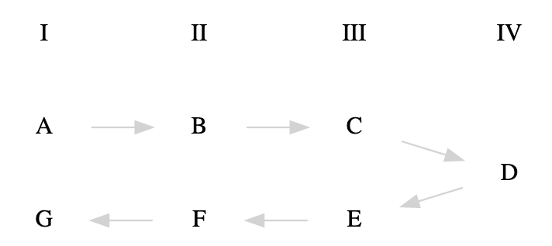
\includegraphics{chapters/02_Structure/images/image1.png}

}

\caption{The Standard Sequence as a Narrative Arc}

\end{figure}

To be sure, the middle chapter plays a central role in our story. If we
think of the story as following a classical ``there and back again''
structure---a chiasmus pattern like \(X_1, Y_1, Z, Y_2, X_2\)---then
chapter \(D\) is the pivot, while chapters \(A,\) \(B,\) and \(C\)
mirror \(E,\) \(F,\) and \(G\). Thinking of the story in this way allows
us to identify a parallel structure in the pipeline, connecting phases
that are usually seen as separate. Specifically, we may visualize the
pipeline as an arc, a \textbf{U}-shaped process in which chapters in the
first half of the pipeline mirror the those of the second half. We may
then group chapters by the pairs formed in this way, yielding four
zones---\(A\) and \(G\) belong to zone \(I\), \(B\) and \(F\) to \(II\),
\(C\) and \(E\) to \(III\), and \(D\) to \(IV\)---as in the following
diagram:

\begin{figure}

{\centering 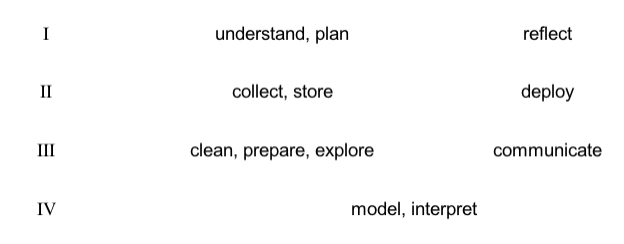
\includegraphics{chapters/02_Structure/images/image2.png}

}

\caption{The Arc Transposed}

\end{figure}

With this visualization, we can discern some interesting properties
about the data science pipeline that are not obvious in the original
sequential image. For one, the arc structure suggests that the two ends
of the pipe are not separate; both make direct contact with the external
world (relative to the internal world of the pipeline considered as a
system). The external world---natural or social---from which data are
pulled is the same world into which data products are inserted. This
insight echoes the CRISP-DM model, which connects \(A\) and \(G\)
(actually \(F\)), except that the two ends of the arc model are not
directly connected. Instead, they come into contact with---and are
separated by---the world in all of its complexity and unpredictability.
The relationship between the effects caused by our data products \(G\)
and the data we pull from the world \(A\) is not given but a matter of
discovery---and often surprise. This is an important distinction between
the model being proposed here and the simple idea that the pipeline
forms a closed circle.

\hypertarget{interpreting-the-themes}{%
\chapter{Interpreting the Themes}\label{interpreting-the-themes}}

At this point, we can explore the unifying themes associated with the
four zones in our arc model by transposing the preceding visualization,
which draws attention to what is common to each pairing. This generates
four candidate areas of data science expertise---activities that,
although they appear on opposite ends of the pipeline, nevertheless
share basic knowledge, know-how, and areas of concern.

Zone \(IV\) is the easiest to interpret in this way because as the pivot
of the arc it is not paired. It represents the work of modeling a
problem mathematically, as well as evaluating and interpreting the
results of mathematical modeling. This work requires data to be
available in a particular form---clean and organized, usually as
``tidy'' analytical tables---and it produces results that need to be
prepared for consumption by non-specialists. As stated above, it is the
pivot of the arc, the core process, where the prior phases constitute
pre-processing and following phases post-processing.

Zone \(I\) is also relatively easy to interpret: the functions in this
group each involve understanding the relationship between the pipeline
and the external world, the messy interface between the enterprise of
data science and the variety of real world situations in which it
operates and impacts. Again, this relationship has a dual character,
based on the difference between input and output, reading from and
writing to the world. Note also that there is an open-ended quality to
the this relationship that is elided by circular representations---there
is always a knowledge gap between one's understanding of a data product
and its real effects on the world, effects which may in turn influence
source data.

We may note in passing that \(I\) and \(IV\) can be contrasted in
several ways---external vs internal, messy vs clean, exoteric vs
esoteric, qualitative vs quantitative, existential vs essential,
concrete vs abstract, periphery vs center, etc.

When it comes to zones \(II\) and \(III\), the interpretation of results
is less straightforward. This is because the reality of the kind of work
performed in these areas is not as clear-cut as it is for \(I\) and
\(IV\). Both \(II\) and \(III\) exhibit an internal complexity not found
in the others, and the two are less clearly separable from each other
than they are from the other two. One reason for this complexity is that
here pure and applied forms of knowledge intermingle in ways that defy
easy description from an academic perspective.

For example, the work of ``data wrangling,'' often considered essential
to data science, spans the two domains and involves a complex mixture of
specific technological know-how and general scientific principles. It
turns out that the relationship between these kinds of knowledge is
highly contested, as evidenced by the reception of Donoho's ``50 Years
of Data Science,'' which has been criticized for separating science from
engineering and demoting the importance of the latter (Donoho 2017).
Regardless of the validity of this criticism, there is without doubt a
long-standing conflict between computational data mining and statistical
data analysis over what counts as valid forms of knowledge, and this
conflict emerges in the representation of zones \(II\) and \(III\) we
find in our corpus.

We can take the conflict of interpretations over the status of technical
knowledge in data science as a clue and use it to identify two broad
dimensions that cross-cut the functions in zones \(II\) and \$III\$:
technical know-how and abstract representation. We can reassign our
labels to these dimensions, using the prime notation of \(II'\) and
\(III'\) to indicate that they are transformation of our original
themes.

Technical know-how \(II´\) involves expertise in developing and
deploying software and hardware designed to handle data at scale,
including high-performance computing, big data architectures (such as
Hadoop and its descendants), and data-oriented programming languages and
libraries. The topics associated with \(II'\) are highly specific and
change rapidly relative to other forms of knowledge, and so are often
omitted from, or under-represented in, academic curricula, even though
to many they are the \emph{sine qua non} of data science.

Abstract representation \(III´\), on the other hand, involves expertise
in areas ranging from how data are to be modeled for capture and
analysis to how the results of analyses are to be presented to
non-expert decision-makers. These areas of knowledge strive for formal
generality over the long run; they are often expressed as grammars or
design languages, frequently with visual modes (such as
entity-relationship models and unified modeling language UML). They also
include other forms of visualization, such as the plots developed for
exploratory data analysis, such as box plots, and those used to
represent statistical facts and analytical results in dashboards and
infographics.

\hypertarget{the-four-areas-plus-one}{%
\chapter{The Four Areas, Plus One}\label{the-four-areas-plus-one}}

We are now ready to define and name the areas of data science expertise
that emerge from an analysis of the pipeline considered as an arc. In
each case, we want to identify the common context shared by the paired
activities in each zone as well as the tension that exists between them
by virtue of their occupying opposite sides of the pipeline. In many
cases, although we can identify a shared theme in each zone's work, the
reality is that practitioners do not always interact or share
disciplinary homes. One of the benefits of this model will be to
identify these points of synergy and to identify new disciplinary
boundaries.

\textbf{Area I: Value}

The area of value is defined by the relationship of data science to the
world from which it draws data and into which it inserts data products.
More broadly, it concerns the primary motivations of data science---why
do we practice data science in the first place? It combines the
traditional discipline of ethics with the professional activities of
business planning, policy making, developing motivations for scientific
research, and other activities that have a direct impact on people and
the planet. This is the area where we determine what we do versus what
we do not do, in order to maximize societal and environmental benefit
and minimize harm. It is also the area that looks inward to the other
data science areas and provides guidance on such issues as algorithmic
bias or open science. Common activities include the forming of value
propositions that initiate data science projects, research into how data
is created and used ``in the wild,'' understanding the ethics of data
acquisition, manipulation, communication, and sharing, and the
application of data products in the world.

\textbf{Area II´: Design}

The area of design is defined by the relationship between human and
machine forms of representation. This relationship is bidirectional:
human-generated data flowing into the pipeline must be represented for
machine consumption (H2M, or \(H \rightarrow M\)), while analytically
transformed data going out must be represented for human consumption
(M2H, or \(M \rightarrow H\)). This area therefore includes expertise in
human-machine interaction as it appears at the points of both consuming
data and producing data products. Activities here include the
representation and communication of captured data for the work of
analytics, e.g.~in database modeling, the curation of data, and of
complex data and analytical results to humans to drive decision-making
and influence behavior. It also includes the making of things, with
purpose (i.e.~to solve problems) and intent (meaning, concision, focus).
A key part of the area is the broad practice of what is often called
visualization, the translation of complex quantitative information into
visual (and other sensory) forms that non-experts can understand. In
slightly more technical terms, the area of design focuses on what Zuboff
called ``informating,'' the process by which the world is represented
for computation and analytics, and also by which analytical models and
results are represented to the world (Zuboff 1995). These two processes
often produce competing representations---a private one \emph{of} the
world for the data scientist, and a public one \emph{for} the world of
the results of analytics. One task of this area is to reconcile these
two representations.

\textbf{Area III´: Systems}

The area of systems is defined by the technological infrastructure that
is common to the pipeline but concentrated in the activities of
wrangling data, deploying data products, and building out systems to
support these activities at scale. This area includes expertise in
infrastructure systems and architectures to support working with big
data---big in terms of volume, velocity, and variety---and building high
performance systems in both development and production environments. It
includes the broad areas of hardware and software as such---computer
technology as opposed to computer science. Key activities include
developing cloud resources, building performant pipelines to ingest and
aggregate data, developing networks of resilient distributed data, and
writing and using software to accomplish tasks. This area is often
referred to as ``data engineering'' or ``machine learning engineering,''
which, according to Owen, ``is most of what Data Science is and
Statistics is not'' (Owen 2015).

\textbf{Area IV: Analytics}

The area of analytics is defined by the practice of mathematical
modeling based on data. This area includes what many consider to be the
essence of data science, the combination of statistical methods with
machine learning, along with information theory, optimization, network
analysis, complexity theory, simulations, and other rigorous
quantitative methods from a variety of fields. Although unified by a
broad commitment to advanced mathematical models and computational
algorithms, in reality this is a heterogeneous collection of competing
schools and methods. Tensions include inference vs prediction,
parametric vs non-parametric (kernel-based) methods, frequentist vs
Bayesian statistics, analytic vs algorithmic solutions (including
simulations), etc. Key activities include clustering, pattern
recognition, regression, rule mining, feature engineering, model
selection, performance evaluation, and a host of other activities.
Although currently dominated by statistical methods, this area also
includes the rule-based methods that dominated the field of artificial
intelligence before the more recent successes of statistical learning
and deep learning.

\textbf{Area V: Practice}

The preceding four areas each represent areas of foundational knowledge,
forms of expertise that can be taught as more or less separate subjects.
In practice, however, these areas represent the interlocking parts of a
division of labor that are integrated in the pipeline. This area
consists of actual activities that brings people together to combine
expertise from each of the four areas. It is characterized by data
science teams working together and with external parties to develop
solutions and projects that are responsible, authentic, efficient, and
effective. Practice is also where the core areas of data science come
into contact with a broad spectrum of domain knowledge and real world
problems. The following diagram shows the central, integrative role
played by practice:

\begin{figure}

{\centering 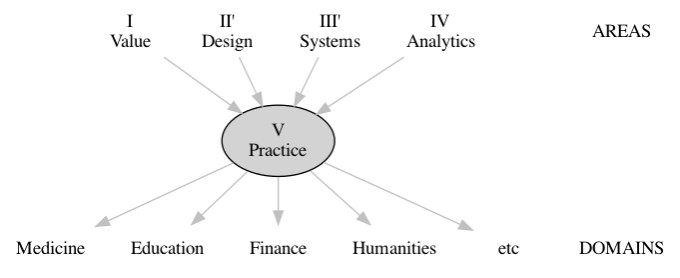
\includegraphics{chapters/02_Structure/images/image3.png}

}

\caption{The Integrative Role of Practice}

\end{figure}

\hypertarget{two-principal-components}{%
\chapter{Two Principal Components}\label{two-principal-components}}

Is there a way to understand how the four primary areas are related to
each other, beyond their being composed of functions from the same
pipeline? Put another way, does the pipeline-as-arc model exhibit any
structural features that will help us conceptualize the broader space of
data science? Two such features stand out: (1) the opposition between
concrete and abstract forms of representation, and (2) between human and
machine processing.

Regarding the concrete and the abstract, it's clear that the arc model
has a metric quality to it: as one moves toward the pivot point of
analysis, one moves away from the concrete messiness of reality as
experienced to the ``tidy'' and abstract world of mathematics;
similarly, as one moves from the pivot back to the world, there is a
requirement to convert esoteric results into more humanly intelligible
forms, often through a process of concretization; visualizations succeed
by employing concrete metaphors that flesh out mathematical ideas that
are notoriously detached from the imagination---no one can imagine, for
example, n-dimensional spaces beyond a handful of dimensions. The arc
describes a dialectic of abstraction and concretization that defines the
ebb and flow and data science work.

\begin{longtable}[]{@{}lll@{}}
\toprule()
~ & Concrete & Abstract \\
\midrule()
\endhead
Human & IVALUE & II'DESIGN \\
Machine & III'SYSTEMS & IVANALYTICS \\
\bottomrule()
\end{longtable}

The Four Areas in Two Dimensions

The dimension of human and machine processing exhibits a similar
duality, that between the conversion of information from humanly
accessible forms, such as given by data acquired by instruments, into
machine readable and processible forms, and the reverse. The process of
moving from human to machine representations is a large part of what
data capture, modeling, and wrangling is all about, while the process of
converting the results of machine learning, broadly conceived, into
humanly actionable form is what visualization and productization are all
about. The reality of this dualism is captured by the concept of
human-computer interaction (HCI), an established field that is
applicable to both sides of the arc.

How do the four fundamental areas map onto these two dimensions? We can
define each area as a combination of one pole from each duality; the
four areas result from all possible permutations of the two dimensions.
This produces the following high level characterizations of each area:
(1) Value is concerned with concrete humanity, (2) Design with abstract
humanity, (3) Analytics with abstract machinery, and (4) Systems is
concerned with concrete machinery. All of these make intuitive sense,
with the exception of Design. This is consistent, however, with the fact
that the area of Design emerges from this analysis as an undervalued and
not well understood area of expertise, even though Yau emphasized it
early on (Yau 2009b). Indeed, one of the consequences of this analysis
is to train our attention on this area of knowledge and to develop it
further.

One exciting interpretation of the two dimensions defined here is that
they correspond to two principal components that undergird the general
field of data science. As components, these axes define two orthogonal
dimensions within which all the specific topics of data science may, in
principle, be plotted. The reality behind these axes may be that they
represent cognitive styles associated with the division of labor implied
by the data science pipeline.

\textbf{PC1: Human versus Machine}

The human-machine axis accounts for the most variance in the field. This
seems evident from the fact that Conway's Venn diagram model of data
science represents only the machine side of our model, with practice
replaced by ``substantive expertise'' (Conway 2010). The human
side---Value and Design---is left out, or short-changed by being lumped
in with domain knowledge. The very fact that the human side has to be
explained and added to the model suggests strongly that it defines a
pole at some distance from the areas of knowledge described in Conway's
model. The human pole refers to humanity understood as situated in their
historical, social, and cultural milieu. It is synonymous with
\emph{human experience}. The machine pole refers to the technoscientific
apparatus of formal, quantitative reasoning that operates on
representations of the human and the world. In the context of data
science, it is more or less synonymous with \emph{machine intelligence},
broadly conceived to include machine learning but also other modes of
analysis on the spectrum of prediction and inference. Given these poles,
the human-machine axis represents the opposition between humanistic
disciplines that seek to understand human experience as such, and the
formal sciences that employ machine intelligence, broadly conceived, to
interpret that experience as represented and aggregated in the form of
data.

\textbf{PC2: Concrete versus Abstract}

The abstract-concrete axis accounts for the difference between two forms
of knowledge, roughly between direct experience and the indirect
representation of that experience enabled through data. Both the realm
of Value and Systems involve immersion in the messy details of lived
experience---and direct acquaintance with the devils in those details.
This is the messy world of hacks and ironies. The realms of Design and
Analysis, on the other hand, are founded on abstract representations
that strive for clear and distinct purity, and which allow for deductive
reasoning to succeed at the cost of simplifying assumptions and reduced
representations. This is the orderly world of models. The concrete pole
refers to situated knowledge, knowledge as understood by hackers and
makers, but also ethnographers who seek to maximize thick description in
their work. It represents \emph{concrete materiality}. The abstract pole
refers to formal knowledge, knowledge in the form of mathematical
symbolism, deductive proofs, and algorithmic patterns. It is
\emph{abstract form}. Given these poles, the concrete-abstract axis is
roughly the opposition between applied and pure forms of knowledge,
between those that embrace materiality and those that seek purity of
form.

\hypertarget{final-representation}{%
\chapter{Final Representation}\label{final-representation}}

The result of the preceding may be represented by the following graphic.

\begin{figure}

{\centering 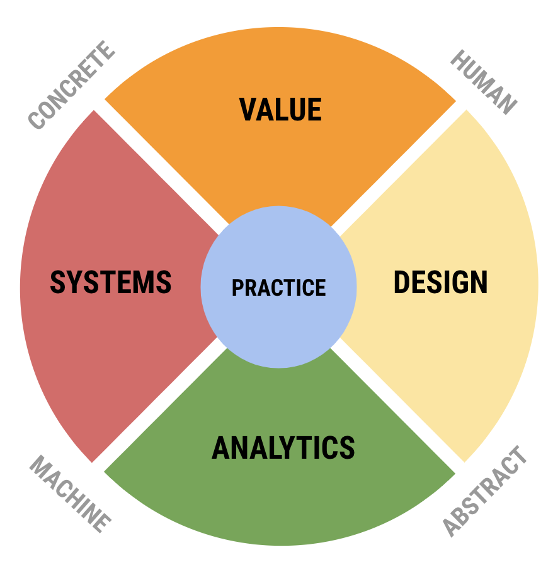
\includegraphics{chapters/02_Structure/images/image5.png}

}

\caption{The 4+1 Model of Data Science}

\end{figure}

This visualization represents data science as composed of specific and
complementary forms of knowledge. The vertical axis defines the dominant
polarity between analysis---the \emph{how} of data science, often
identified entirely with it, contrasted with the \emph{why} of data
science, from which data science derives its meaning and value as a
profession. The horizontal access defines the polarity of methods that
are often obscured in academic definitions of data science---the
supporting practices that make the Analytics component work in the first
place.

\hypertarget{relation-to-ai}{%
\chapter{Relation to AI}\label{relation-to-ai}}

The four areas of data science defined here are surprisingly analogous
to the four approaches to artificial intelligence defined by Russel and
Norvig in their classic textbook on the subject (Russell and Norvig
1995: 5). Their four part model was generated by combining the axes
\(thinking \leftrightarrow acting\) with
\(human \leftrightarrow rational\) as follows:

\begin{longtable}[]{@{}lll@{}}
\toprule()
behavior & mode & systems \\
\midrule()
\endhead
thinking & humanly & cognitive models, ontologies \\
thinking & rationally & logic, laws of thought \\
acting & humanly & Turing test, situated action \\
acting & rationally & agents, bots \\
\bottomrule()
\end{longtable}

Now, it is easy to see how the following analogies make sense:

\[
abstract : concrete :: thinking : action
\]

and

\[
human : rational :: human : machine
\]

Or, put in terms of a set of identities:

\begin{longtable}[]{@{}ll@{}}
\toprule()
AI & DS \\
\midrule()
\endhead
abstract & thinking \\
concrete & action \\
human & human \\
rational & machine \\
\bottomrule()
\end{longtable}

So it makes sense to compare the above table with this one for data
science:

\begin{longtable}[]{@{}
  >{\raggedright\arraybackslash}p{(\columnwidth - 6\tabcolsep) * \real{0.1282}}
  >{\raggedright\arraybackslash}p{(\columnwidth - 6\tabcolsep) * \real{0.1154}}
  >{\raggedright\arraybackslash}p{(\columnwidth - 6\tabcolsep) * \real{0.1410}}
  >{\raggedright\arraybackslash}p{(\columnwidth - 6\tabcolsep) * \real{0.6154}}@{}}
\toprule()
\begin{minipage}[b]{\linewidth}\raggedright
level
\end{minipage} & \begin{minipage}[b]{\linewidth}\raggedright
focus
\end{minipage} & \begin{minipage}[b]{\linewidth}\raggedright
area
\end{minipage} & \begin{minipage}[b]{\linewidth}\raggedright
topic
\end{minipage} \\
\midrule()
\endhead
abstract & human & design & ontologies, data models, visualizations \\
abstract & machine & analytics & math, logic, algorithms \\
concrete & human & value & ethics, research questions, value
propositions \\
concrete & machine & systems & hardware, software, security \\
\bottomrule()
\end{longtable}

By comparing last columns of each table we can see that the 4+1 model of
data science and Russell and Norvig's model of artificial intelligence
share the same general space. The difference is that the former defines
kinds of \emph{acquired knowledge}, whereas the latter concerns kinds of
\emph{built systems}.

\hypertarget{concluding-remarks}{%
\chapter{Concluding Remarks}\label{concluding-remarks}}

The point of the 4 + 1 model, abstract as it is, is to provide a
practical template for strategically planning the various elements of a
school of data science. To serve as an effective template, a model must
be general. But generality if often purchased at the cost of intuitive
understanding. The following caveats may help make sense of the model
when considering its usefulness when applied to various concrete
activities.

\textbf{The model describes areas of academic expertise, not objective
reality}. It is a map of a division of labor writ large. Although each
of the areas has clear connections to the others, the question to ask
when deciding where an activity belongs is: \emph{who would be an expert
at doing it}? The realms help refine this question: the analytics area,
for example, contains people who are good at working with abstract
machinery. The four areas have the virtue of isolating intuitively
correct communities of expertise. For example, people who are great at
data product design may not know the esoteric depths of machine
learning, and that adepts at machine learning are not usually experts in
understanding human society and normative culture.

\textbf{Each area in the model contains a collection of subfields that
need to be teased out}. Some areas will have more subfields than others.
Although some areas may be smaller than others in terms of number of
experts (faculty) and courses, each area has a major impact on the
overall practice of data science and the quality of an academic
program's activities. In addition, these subfields are in an important
sense ``more real'' than the categories. We can imagine them forming a
dense network in which the areas define communities with centroids, and
which are more interconnected than the clean-cut image of the model
implies.

\textbf{The principal components abstract/concrete and human/machine are
meant to help imagine the kinds of activities that belong in each area},
through their connotations when combined to form the four bigrams ---
concrete human, abstract human, concrete machine, and abstract machine.
For example, the area of value as the realm of the ``concrete human''
(or perhaps ``concrete humanity'') is meant to connote what the Spanish
philosopher Unamuno called the world of ``flesh and bone'' within which
we live and die, that is, where things matter. On the other hand,
analytics as the realm of the ``abstract machine'' is meant to connote
the platonic world of mathematical reasoning which, since Euclid, has
been characterized by rigorous, abstract, deductive reasoning that has
literally been described as an abstract machine (see Alan Turing).

\textbf{At the center of this model and each area is people}. Even in
the area classified as ``abstract machine,'' people and human thinking
is at the center.

\bookmarksetup{startatroot}

\hypertarget{references}{%
\chapter*{References}\label{references}}
\addcontentsline{toc}{chapter}{References}

\markboth{References}{References}

\hypertarget{refs}{}
\begin{CSLReferences}{1}{0}
\leavevmode\vadjust pre{\hypertarget{ref-afcrl1963}{}}%
AFCRL. 1963. {``Report on Research at AFCRL: July 1962 - July 1963.''}
Bedford, Mass.

\leavevmode\vadjust pre{\hypertarget{ref-afcrl1967}{}}%
---------. 1967. {``Report on Research at AFCRL: July 1965 - June
1967.''} Bedford, Massachusetts.

\leavevmode\vadjust pre{\hypertarget{ref-afcrl1970}{}}%
---------. 1970. {``Report on Research at AFCRL: July 1967 {\textendash}
June 1970.''} Bedford, Massachusetts.

\leavevmode\vadjust pre{\hypertarget{ref-afcrl1973}{}}%
---------. 1973. {``Report on Research at AFCRL: July 1970 - June
1972.''}

\leavevmode\vadjust pre{\hypertarget{ref-altshuler2013}{}}%
Altshuler, Edward E. 2013. \emph{The Rise and Fall of Air Force
Cambridge Research Laboratories}. CreateSpace Independent Publishing
Platform.

\leavevmode\vadjust pre{\hypertarget{ref-alvarado2017}{}}%
Alvarado, Rafael, and Paul Humphreys. 2017. {``Big Data, Thick
Mediation, and Representational Opacity.''} \emph{New Literary History}
48 (4): 729--49. \url{https://doi.org/10.1353/nlh.2017.0037}.

\leavevmode\vadjust pre{\hypertarget{ref-anderson2008}{}}%
Anderson, Chris. 2008. {``The End of Theory: The Data Deluge Makes the
Scientific Method Obsolete.''} \emph{Wired} 16 (June).
\url{http://www.wired.com/science/discoveries/magazine/16-07/pb_theory}.

\leavevmode\vadjust pre{\hypertarget{ref-ando1966}{}}%
Ando, A., and G. M. Kaufman. 1966. {``Evaluation of an Ad Hoc Procedure
for Estimating Parameters of Some Linear Models.''} \emph{The Review of
Economics and Statistics} 48 (3): 334--40.
\url{https://doi.org/10.2307/1927089}.

\leavevmode\vadjust pre{\hypertarget{ref-announce1964}{}}%
{``Announcements.''} 1964. \emph{Nature} 203 (4952): 1337--37.
\url{https://doi.org/10.1038/2031337d0}.

\leavevmode\vadjust pre{\hypertarget{ref-appropriations1958}{}}%
Appropriations, United States Congress House. 1958. \emph{Second
Supplemental Appropriation Bill: 1958, Hearings ... 85th Congress, 2d
Session}.

\leavevmode\vadjust pre{\hypertarget{ref-appropriations1970}{}}%
Appropriations, United States Congress House Committee on. 1970.
\emph{Department of Defense Appropriations for 1971: Hearings ...
Ninety-First Congress, Second Session}. U.S. Government Printing Office.

\leavevmode\vadjust pre{\hypertarget{ref-asastat2015}{}}%
{``ASA Statement on the Role of Statistics in Data Science.''} 2015,
August.

\leavevmode\vadjust pre{\hypertarget{ref-baier2006}{}}%
Baier, Daniel, and Klaus-Dieter Wernecke. 2006. \emph{Innovations in
Classification, Data Science, and Information Systems: Proceedings of
the 27th Annual Conference of the Gesellschaft Für Klassifikation e.V.,
Brandenburg University of Technology, Cottbus, March 12-14, 2003}.
Springer Science \& Business Media.

\leavevmode\vadjust pre{\hypertarget{ref-bell2007}{}}%
Bell, Gordon, Jim Gray, and Alex Szalay. 2007. {``Petascale
Computational Systems.''} \emph{arXiv:cs/0701165}, January.
\url{http://arxiv.org/abs/cs/0701165}.

\leavevmode\vadjust pre{\hypertarget{ref-berners-lee2008}{}}%
Berners-Lee, Tim, and Mark Fischetti. 2008. \emph{Weaving the Web: The
Original Design and Ultimate Destiny of the World Wide Web by Its
Inventor}. Paw Prints.

\leavevmode\vadjust pre{\hypertarget{ref-bock2001}{}}%
Bock, Hans-Hermann. 2001. {``A History of the International Federation
of Classification Societies.''}

\leavevmode\vadjust pre{\hypertarget{ref-borne2009}{}}%
Borne, Kirk D., Suzanne Jacoby, K. Carney, A. Connolly, T. Eastman, M.
J. Raddick, J. A. Tyson, and J. Wallin. 2009. {``The Revolution in
Astronomy Education: Data Science for the Masses.''}
\emph{arXiv:0909.3895 {[}Astro-Ph, Physics:physics{]}}, September.
\url{http://arxiv.org/abs/0909.3895}.

\leavevmode\vadjust pre{\hypertarget{ref-breiman2001}{}}%
Breiman, Leo. 2001. {``Statistical Modeling: The Two Cultures.''}
\emph{Statistical Science} 16 (3): 199--231.
\url{https://doi.org/10.1214/ss/1009213726}.

\leavevmode\vadjust pre{\hypertarget{ref-breiman1976}{}}%
Breiman, L., and W. S. Meisel. 1976. {``General Estimates of the
Intrinsic Variability of Data in Nonlinear Regression Models.''}
\emph{Journal of the American Statistical Association} 71 (354): 301--7.
\url{https://doi.org/10.2307/2285301}.

\leavevmode\vadjust pre{\hypertarget{ref-bryan2017}{}}%
Bryan, Jennifer, and Hadley Wickham. 2017. {``Data Science: A Three Ring
Circus or a Big Tent?''} December.
\url{https://arxiv.org/abs/1712.07349v1}.

\leavevmode\vadjust pre{\hypertarget{ref-bryce2001}{}}%
Bryce, G. Rex, Robert Gould, William I. Notz, and Roxy L. Peck. 2001.
{``Curriculum Guidelines for Bachelor of Science Degrees in Statistical
Science.''} \emph{The American Statistician} 55 (1): 7--13.
\url{https://www.jstor.org/stable/2685523}.

\leavevmode\vadjust pre{\hypertarget{ref-chambersGreaterLesserStatistics1993}{}}%
Chambers, John M. 1993. {``Greater or {Lesser Statistics}: {A Choice}
for {Future Research}.''} \emph{Statistics and Computing} 3 (4):
182--84. \url{https://doi.org/10.1007/BF00141776}.

\leavevmode\vadjust pre{\hypertarget{ref-chynoweth2008}{}}%
Chynoweth, Carly. 2008. {``Communication Is Key for Programmers.''}
\emph{The Times}, May.
\url{https://advance.lexis.com/document/?pdmfid=1516831\&crid=e0aaeba2-6f62-410b-bc54-a11d5f8f5253\&pddocfullpath=\%2Fshared\%2Fdocument\%2Fnews\%2Furn\%3AcontentItem\%3A4SFX-GS40-TX38-S09K-00000-00\&pdcontentcomponentid=10939\&pdteaserkey=sr30\&pditab=allpods\&ecomp=gb63k\&earg=sr30\&prid=19e1f7de-2617-49de-93da-706f9a17e95e}.

\leavevmode\vadjust pre{\hypertarget{ref-cleveland2001}{}}%
Cleveland, William S. 2001. {``Data Science: An Action Plan for
Expanding the Technical Areas of the Field of Statistics.''}
\emph{International Statistical Review / Revue Internationale de
Statistique} 69 (1): 21--26. \url{https://doi.org/10.2307/1403527}.

\leavevmode\vadjust pre{\hypertarget{ref-codd1970}{}}%
Codd, Edgar F. 1970. {``A Relational Model of Data for Large Shared Data
Banks.''} \emph{Communications of the ACM} 13 (6): 377387.
\url{http://dl.acm.org/citation.cfm?id=362685}.

\leavevmode\vadjust pre{\hypertarget{ref-CommunityClevernessRequired2008}{}}%
{``Community Cleverness Required.''} 2008. \emph{Nature} 455 (7209):
1--1. \url{https://doi.org/10.1038/455001a}.

\leavevmode\vadjust pre{\hypertarget{ref-computer1975}{}}%
\emph{Computers in Education: Proceedings of the IFIP ... World
Conference}. 1975. North-Holland Publishing Company.

\leavevmode\vadjust pre{\hypertarget{ref-conway2010}{}}%
Conway, Drew. 2010. {``The Data Science Venn Diagram.''}
\url{http://drewconway.com/zia/2013/3/26/the-data-science-venn-diagram}.

\leavevmode\vadjust pre{\hypertarget{ref-corliss1967}{}}%
Corliss, William R. 1967. \emph{Scientific Satellites}. Scientific;
Technical Information Division, National Aeronautics; Space
Administration.

\leavevmode\vadjust pre{\hypertarget{ref-crawfordjr.1974}{}}%
Crawford, Jr., Perry. 1974. {``On the Connections Between Data and
Things in the Real World.''} In, 51--57.

\leavevmode\vadjust pre{\hypertarget{ref-datasci}{}}%
{``Data Science Journal.''} n.d. \url{http://datascience.codata.org/}.

\leavevmode\vadjust pre{\hypertarget{ref-davenport2012}{}}%
Davenport, Thomas H., and D. J. Patil. 2012. {``Data Scientist: The
Sexiest Job of the 21st Century.''}
\url{https://hbr.org/2012/10/data-scientist-the-sexiest-job-of-the-21st-century}.

\leavevmode\vadjust pre{\hypertarget{ref-davidian2013}{}}%
Davidian, Marie. 2013. {``Aren't We Data Science?''} \emph{AMSTAT news:
the membership magazine of the American Statistical Association}, no.
433: 3.
\url{https://dialnet.unirioja.es/servlet/articulo?codigo=4331554}.

\leavevmode\vadjust pre{\hypertarget{ref-davis}{}}%
Davis, Miriam. n.d. {``The Canary That Forgot Its Song.''}

\leavevmode\vadjust pre{\hypertarget{ref-deboeck1999}{}}%
DeBoeck, Paul. 1999. {``International Federation of Classification
Societes Newsletter,''} January.

\leavevmode\vadjust pre{\hypertarget{ref-demchenko2017}{}}%
Demchenko, Yuri. 2017. {``The Emerging Role of the Data Scientist and
the Experience of Data Science Education at the University of
Amsterdam.''} In.

\leavevmode\vadjust pre{\hypertarget{ref-dharDataSciencePrediction2013}{}}%
Dhar, Vasant. 2013. {``Data Science and Prediction.''}
\emph{Communications of the ACM} 56 (12): 64--73.
\url{https://doi.org/10.1145/2500499}.

\leavevmode\vadjust pre{\hypertarget{ref-donoho2017}{}}%
Donoho, David. 2017. {``50 Years of Data Science.''} \emph{Journal of
Computational and Graphical Statistics} 26 (4): 745--66.
\url{https://doi.org/10.1080/10618600.2017.1384734}.

\leavevmode\vadjust pre{\hypertarget{ref-driscoll2009}{}}%
Driscoll, Michael E. 2009. {``The Three Sexy Skills of Data Geeks.''}
\url{https://web.archive.org/web/20090530074011/dataspora.com/blog/sexy-data-geeks/}.

\leavevmode\vadjust pre{\hypertarget{ref-fayyad1996}{}}%
Fayyad, Usama M., Gregory Piatetsky-Shapiro, and Padhraic Smyth. 1996.
{``From Data Mining to Knowledge Discovery: An Overview.''} In, 134.
USA: American Association for Artificial Intelligence.

\leavevmode\vadjust pre{\hypertarget{ref-friedman1997}{}}%
Friedman, Jerome H. 1997. {``Data Mining and Statistics: What's the
Connection?''}
\url{https://www.academia.edu/28735089/Data_Mining_and_Statistics_Whats_the_Connection}.

\leavevmode\vadjust pre{\hypertarget{ref-fry2004}{}}%
Fry, Benjamin Jotham. 2004. {``Computational Information Design.''} PhD
thesis. \url{https://dspace.mit.edu/handle/1721.1/26913}.

\leavevmode\vadjust pre{\hypertarget{ref-garfinkel2000}{}}%
Garfinkel, Simson. 2000. \emph{Database Nation: The Death of Privacy in
the 21st Century}. O'Reilly Media, Inc.

\leavevmode\vadjust pre{\hypertarget{ref-goldfarb1970}{}}%
Goldfarb, C. F. 1970. {``An Online System for Integrated Text
Processing.''} \emph{Proceedings of the American Society for Information
Science} 7: 147--50. \url{https://ci.nii.ac.jp/naid/10012384147/}.

\leavevmode\vadjust pre{\hypertarget{ref-ifipgui1971}{}}%
Gould, I. H., ed. 1971. \emph{IFIP Guide to Concepts and Terms in Data
Processing}. Vol. 2. London: North-Holland.
\url{https://www.google.com/books/edition/IFIP_Guide_to_Concepts_and_Terms_in_Data/S9C7AAAAIAAJ?hl=en\&gbpv=0}.

\leavevmode\vadjust pre{\hypertarget{ref-halevy2009}{}}%
Halevy, Alon, Peter Norvig, and Fernando Pereira. 2009. {``The
Unreasonable Effectiveness of Data.''} \emph{IEEE Intelligent Systems}
24 (2): 812.
\url{https://ieeexplore.ieee.org/abstract/document/4804817}.

\leavevmode\vadjust pre{\hypertarget{ref-hammerbacher2009}{}}%
Hammerbacher, Jeff. 2009. {``Information Platforms and the Rise of the
Data Scientist.''} In, 7384. O'Reilly Media Sebastopol, CA.

\leavevmode\vadjust pre{\hypertarget{ref-hayashi1998}{}}%
Hayashi, Chikio. 1998b. \emph{Data Science, Classification, and Related
Methods: Proceedings of the Fifth Conference of the International
Federation of Classification Societies (IFCS-96), Kobe, Japan, March
27-30, 1996}. Kobe, Japan: Springer.

\leavevmode\vadjust pre{\hypertarget{ref-hayashi1998a}{}}%
---------. 1998a. \emph{Data Science, Classification, and Related
Methods: Proceedings of the Fifth Conference of the International
Federation of Classification Societies (IFCS-96), Kobe, Japan, March
27-30, 1996}. Kobe, Japan: Springer.

\leavevmode\vadjust pre{\hypertarget{ref-hendry1995}{}}%
Hendry, David F. 1995. \emph{Dynamic Econometrics}. Advanced Texts in
Econometrics. New York: Oxford Univ Press.
\url{https://www.google.com/books/edition/Dynamic_Econometrics/XcWVN2-2ZqIC?hl=en\&gbpv=1\&dq=\%22data+mining\%22\&pg=PA544\&printsec=frontcover}.

\leavevmode\vadjust pre{\hypertarget{ref-herman2013}{}}%
Herman, Mark, Stephanie Rivera, Mills Stephen, Josh Sullivan, Peter
Guerra, Alex Cosmas, Drew Farris, et al. 2013. {``Field Guide to Data
Science.''}
\url{https://www.boozallen.com/s/insight/publication/field-guide-to-data-science.html}.

\leavevmode\vadjust pre{\hypertarget{ref-hey2009}{}}%
Hey, Tony, Stewart Tansley, and Kristin Tolle. 2009. \emph{The Fourth
Paradigm: Data-Intensive Scientific Discovery}.
\url{https://www.microsoft.com/en-us/research/publication/fourth-paradigm-data-intensive-scientific-discovery/}.

\leavevmode\vadjust pre{\hypertarget{ref-higgins1999}{}}%
Higgins, James J. 1999. {``Nonmathematical Statistics: A New Direction
for the Undergraduate Discipline.''} \emph{The American Statistician} 53
(1): 1--6. \url{https://doi.org/10.1080/00031305.1999.10474418}.

\leavevmode\vadjust pre{\hypertarget{ref-89618ac5-1e4e-3cce-a5de-eb7b926f27c9}{}}%
Kettenring, Jon R. 1997a. {``Shaping Statistics for Success in the 21st
Century.''} \emph{Journal of the American Statistical Association} 92
(440): 12291234. \url{http://www.jstor.org/stable/2965390}.

\leavevmode\vadjust pre{\hypertarget{ref-kettenring1997a}{}}%
---------. 1997b. {``Shaping Statistics for Success in the 21st
Century.''} \emph{Journal of the American Statistical Association} 92
(440): 1229--34. \url{https://doi.org/10.1080/01621459.1997.10473641}.

\leavevmode\vadjust pre{\hypertarget{ref-kusnetzky2010}{}}%
Kusnetzky, Dan. 2010. {``What Is {"}Big Data?{"}.''} \emph{ZDNet},
February.
\url{http://www.zdnet.com/blog/virtualization/what-is-big-data/1708}.

\leavevmode\vadjust pre{\hypertarget{ref-laney2001}{}}%
Laney, Doug. 2001. {``3d Data Management: Controlling Data Volume,
Velocity and Variety.''} \emph{META Group Research Note} 6: 70.

\leavevmode\vadjust pre{\hypertarget{ref-laney2012}{}}%
---------. 2012. {``Defining and Differentiating the Role of the Data
Scientist.''}
\url{https://web.archive.org/web/20120327163714/http://blogs.gartner.com/doug-laney/defining-and-differentiating-the-role-of-the-data-scientist/}.

\leavevmode\vadjust pre{\hypertarget{ref-luxe9vi-strauss1955}{}}%
Lévi-Strauss, Claude. 1955. {``The Structural Study of Myth.''}
\emph{The Journal of American Folklore} 68 (270): 428--44.
\url{https://doi.org/10.2307/536768}.

\leavevmode\vadjust pre{\hypertarget{ref-lide2012}{}}%
Lide, David R., and Gordon H. Wood. 2012. \emph{CODATA @ 45 Years: The
Story of the ICSU Committee on Data for Science and Technology (CODATA)
from 1966 to 2010}. Paris, France: CODATA.
\url{https://books.google.com/books/about/CODATA_45_Years.html?id=NjA8kgEACAAJ\&utm_source=gb-gplus-shareCODATA}.

\leavevmode\vadjust pre{\hypertarget{ref-lohr2009}{}}%
Lohr, Steve. 2009. {``For Today{'}s Graduate, Just One Word:
Statistics.''} \emph{The New York Times}, August.
\url{https://www.nytimes.com/2009/08/06/technology/06stats.html}.

\leavevmode\vadjust pre{\hypertarget{ref-lohr2014}{}}%
---------. 2014. {``For Big-Data Scientists, {`}Janitor Work{'} Is Key
Hurdle to Insights.''} \emph{The New York Times}, August.
\url{https://www.nytimes.com/2014/08/18/technology/for-big-data-scientists-hurdle-to-insights-is-janitor-work.html}.

\leavevmode\vadjust pre{\hypertarget{ref-loukides2011}{}}%
Loukides, Mike. 2011. \emph{What Is Data Science?} {"}O'Reilly Media,
Inc.{"}.

\leavevmode\vadjust pre{\hypertarget{ref-lovell1983}{}}%
Lovell, Michael C. 1983. {``Data Mining.''} \emph{The Review of
Economics and Statistics} 65 (1): 1--12.
\url{https://doi.org/10.2307/1924403}.

\leavevmode\vadjust pre{\hypertarget{ref-mason2010}{}}%
Mason, Hilary, and Christopher Wiggins. 2010. {``A Taxonomy of Data
Science.''}
\url{http://www.dataists.com/2010/09/a-taxonomy-of-data-science/}.

\leavevmode\vadjust pre{\hypertarget{ref-mckinseycompany2009}{}}%
McKinsey \& Company. 2009. {``Hal Varian on How the Web Challenges
Managers.''} \emph{McKinsey \& Company}, January.
\url{https://www.mckinsey.com/industries/technology-media-and-telecommunications/our-insights/hal-varian-on-how-the-web-challenges-managers}.

\leavevmode\vadjust pre{\hypertarget{ref-miller2013}{}}%
Miller, Claire Cain. 2013. {``Data Science: The Numbers of Our Lives.''}
\emph{The New York Times}, April.
\url{https://www.nytimes.com/2013/04/14/education/edlife/universities-offer-courses-in-a-hot-new-field-data-science.html}.

\leavevmode\vadjust pre{\hypertarget{ref-mohawkd1966}{}}%
{``Mohawk Data Sciences.''} 1966. \emph{The New York Times}, July.
\url{https://www.nytimes.com/1966/07/30/archives/mohawk-data-sciences.html}.

\leavevmode\vadjust pre{\hypertarget{ref-mortcollinsventures}{}}%
Mort Collins Ventures. n.d. {``Bio.''}
\url{http://www.mcollinsventures.com/bio/}.

\leavevmode\vadjust pre{\hypertarget{ref-naur1966}{}}%
Naur, Peter. 1966. {``The Science of Datalogy.''} \emph{Communications
of the ACM} 9 (7): 485. \url{https://doi.org/10.1145/365719.366510}.

\leavevmode\vadjust pre{\hypertarget{ref-naur1968}{}}%
---------. 1968. {``'Datalogy', the Science of Data and Data
Processes.''} In, 13831387.

\leavevmode\vadjust pre{\hypertarget{ref-naur1974}{}}%
---------. 1974. \emph{Concise Survey of Computer Methods}. Petrocelli
Books.

\leavevmode\vadjust pre{\hypertarget{ref-naur1992}{}}%
---------. 1992. \emph{Computing, a Human Activity}. ACM Press.

\leavevmode\vadjust pre{\hypertarget{ref-newscie1992}{}}%
{``New Scientist.''} 1992.

\leavevmode\vadjust pre{\hypertarget{ref-newscie1995a}{}}%
---------. 1995.

\leavevmode\vadjust pre{\hypertarget{ref-newscie1996}{}}%
---------. 1996.

\leavevmode\vadjust pre{\hypertarget{ref-newscie1999}{}}%
---------. 1999.

\leavevmode\vadjust pre{\hypertarget{ref-newscie2001}{}}%
---------. 2001.

\leavevmode\vadjust pre{\hypertarget{ref-office1979}{}}%
Office, Library of Congress Copyright. 1979. \emph{Catalog of Copyright
Entries. Third Series: 1977: July-December: Index}. Copyright Office,
Library of Congress.

\leavevmode\vadjust pre{\hypertarget{ref-ohsumi1992}{}}%
Ohsumi, Noboru. 1992. {``An Experimental System for Navigating
Statistical Meta-Information {\textemdash} The Meta-Stat Navigator.''}
In, edited by Yadolah Dodge and Joe Whittaker, 375--80. Heidelberg:
Physica-Verlag HD. \url{https://doi.org/10.1007/978-3-642-48678-4_48}.

\leavevmode\vadjust pre{\hypertarget{ref-ohsumi1994}{}}%
---------. 1994. {``New Data and New Tools: A Hypermedia Environment for
Navigating Statistical Knowledge in Data Science.''} In, 45--54. Berlin:
Springer-Verlag.

\leavevmode\vadjust pre{\hypertarget{ref-ohsumi2000}{}}%
---------. 2000. {``From Data Analysis to Data Science.''} In, 329334.
Springer.

\leavevmode\vadjust pre{\hypertarget{ref-ohsumi2002}{}}%
---------. 2002. {``Professor Chikio Hayashi.''} \emph{International
Federation of Classification Societies Newsletter} 24 (December): 3--5.

\leavevmode\vadjust pre{\hypertarget{ref-ohsumi2004}{}}%
---------. 2004. {``IFCS-2004 in Chicago.''} In.
\url{https://www.researchgate.net/publication/268719699_Memories_of_Chikio_Hayashi_and_his_great_achievement_2004}.

\leavevmode\vadjust pre{\hypertarget{ref-owen2015}{}}%
Owen, Sean. 2015. {``What {``}50 Years of Data Science{''} Leaves
Out.''}
\url{https://medium.com/@srowen/what-50-years-of-data-science-leaves-out-2366c9b61d3d}.

\leavevmode\vadjust pre{\hypertarget{ref-parsons2019}{}}%
Parsons, Mark A. 2019. {``Revised Focus and Scope.''} \emph{The Data
Science Journal}, November.
\url{https://codata.org/codata-data-science-journal-revised-focus-and-scope/}.

\leavevmode\vadjust pre{\hypertarget{ref-parzen1977}{}}%
Parzen, Emanuel. 1977. {``Nonparametric Statistical Data Science: A
Unified Approach Based on Density Estimation and Testing for'white
Noise'.''}

\leavevmode\vadjust pre{\hypertarget{ref-parzen1979}{}}%
---------. 1979. {``Nonparametric Statistical Data Modeling.''}
\emph{Journal of the American Statistical Association} 74 (365):
105--21. \url{https://doi.org/10.2307/2286734}.

\leavevmode\vadjust pre{\hypertarget{ref-parzen2013}{}}%
Parzen, Emanuel, and Subhadeep Mukhopadhyay. 2013. {``LP Mixed Data
Science : Outline of Theory.''} \emph{arXiv:1311.0562 {[}Math, Stat{]}},
November. \url{http://arxiv.org/abs/1311.0562}.

\leavevmode\vadjust pre{\hypertarget{ref-patil2011}{}}%
Patil, D. J. 2011. {``Building Data Science Teams.''} \emph{O'Reilly
Radar}, September.
\url{http://radar.oreilly.com/2011/09/building-data-science-teams.html}.

\leavevmode\vadjust pre{\hypertarget{ref-piatetsky-shapiro1991}{}}%
Piatetsky-Shapiro, Gregory. 1991. {``Knowledge Disovery in Real
Databases: A Report on the IJCAI-89 Workshop.''} \emph{AI Magazine} 11
(January): 68--70.
\url{https://www.kdnuggets.com/meetings-past/kdd89/kdd-89-report-aimag.html}.

\leavevmode\vadjust pre{\hypertarget{ref-propp1977}{}}%
Propp, V. I. A, and A. Dundes. 1977. \emph{Morphology of the Folktale}.
University of Texas Press.

\leavevmode\vadjust pre{\hypertarget{ref-rizzi2013}{}}%
Rizzi, Alfredo, Maurizio Vichi, and Hans-Hermann Bock. 2013.
\emph{Advances in Data Science and Classification: Proceedings of the
6th Conference of the International Federation of Classification
Societies (IFCS-98) Università {``}La Sapienza{''}, Rome,
21{\textendash}24 July, 1998}. Springer Science \& Business Media.

\leavevmode\vadjust pre{\hypertarget{ref-roberta}{}}%
{``Robert Allen Obituary (2014) - St. Louis, MO - St. Louis
Post-Dispatch.''} n.d.
\url{https://www.legacy.com/us/obituaries/stltoday/name/robert-allen-obituary?id=3008349}.

\leavevmode\vadjust pre{\hypertarget{ref-rodriguez2012}{}}%
Rodriguez, Robert. 2012. {``Big Data and Better Data.''}
\url{https://magazine.amstat.org/blog/2012/06/01/prescorner/}.

\leavevmode\vadjust pre{\hypertarget{ref-rodriguez2013}{}}%
Rodriguez, Robert, Marie Davidian, and Nathaniel Schenker. 2013. {``The
ASA and Big Data.''}
\url{https://magazine.amstat.org/blog/2013/06/01/the-asa-and-big-data/}.

\leavevmode\vadjust pre{\hypertarget{ref-rooney2012}{}}%
Rooney, Ben. 2012. {``Big Data's Big Problem: Little Talent.''}
\emph{Wall Street Journal}, April.
\url{https://online.wsj.com/article/SB10001424052702304723304577365700368073674.html}.

\leavevmode\vadjust pre{\hypertarget{ref-russell1995}{}}%
Russell, Stuart Jonathan, and Peter Norvig. 1995. \emph{Artificial
Intelligence: A Modern Approach}. Prentice Hall.

\leavevmode\vadjust pre{\hypertarget{ref-schader2012}{}}%
Schader, Martin, Wolfgang A. Gaul, and Maurizio Vichi. 2012.
\emph{Between Data Science and Applied Data Analysis: Proceedings of the
26th Annual Conference of the Gesellschaft Für Klassifikation e.V.,
University of Mannheim, July 22{\textendash}24, 2002}. Springer Science
\& Business Media.

\leavevmode\vadjust pre{\hypertarget{ref-shannon1948}{}}%
Shannon, C. E. 1948. {``A Mathematical Theory of Communication.''}
\emph{Bell Systems Technical Journal} 27: 379423 and 623656.
\url{http://portal.acm.org/citation.cfm?id=584093}.

\leavevmode\vadjust pre{\hypertarget{ref-shapiro2006}{}}%
Shapiro, Ehud, Stuart Rison, Andrew Phillips, Andrew Herbert, Editors,
and Stephen Emmott. 2006. \emph{Towards 2020 Science}. Microsoft.
\url{https://www.microsoft.com/en-us/research/publication/towards-2020-science-2/}.

\leavevmode\vadjust pre{\hypertarget{ref-simberloff2005}{}}%
Simberloff, Daniel, B. C. Barish, K. K. Droegemeier, D. Etter, N.
Fedoroff, K. Ford, L. Lanzerotti, A. Leshner, J. Lubchenco, and M.
Rossmann. 2005. {``Long-Lived Digital Data Collections: Enabling
Research and Education in the 21st Century.''} \emph{National Science
Foundation}.

\leavevmode\vadjust pre{\hypertarget{ref-smith2006}{}}%
Smith, F. 2006. {``Data Science as an Academic Discipline.''} \emph{Data
Science Journal} 5 (0): 163--64.
\url{http://datascience.codata.org/articles/abstract/482/}.

\leavevmode\vadjust pre{\hypertarget{ref-swan2008}{}}%
Swan, Alma, and Sheridan Brown. 2008. {``The Skills, Role and Career
Structure of Data Scientists and Curators: An Assessment of Current
Practice and Future Needs.''} \url{http://repository.jisc.ac.uk/245/}.

\leavevmode\vadjust pre{\hypertarget{ref-tanaka2018}{}}%
Tanaka, Yutaka. 2018. {``Comment: On Closing of English Journal of JSCS
and the Birth of New Journal JJSD.''} \emph{Journal of the Japanese
Society of Computational Statistics} 30 (2): 75--77.
\url{https://doi.org/10.5183/jjscs.1802001_245}.

\leavevmode\vadjust pre{\hypertarget{ref-tukey1962}{}}%
Tukey, John W. 1962. {``The Future of Data Analysis.''} \emph{The Annals
of Mathematical Statistics} 33 (1): 1--67.
\url{http://www.jstor.org/stable/2237638}.

\leavevmode\vadjust pre{\hypertarget{ref-tukey1979}{}}%
---------. 1979. {``Nonparametric Statistical Data Modeling: Comment.''}
\emph{Journal of the American Statistical Association} 74 (365):
121--22. \url{https://doi.org/10.2307/2286735}.

\leavevmode\vadjust pre{\hypertarget{ref-varian2010}{}}%
Varian, Hal R. 2010. {``Computer Mediated Transactions.''}
\emph{American Economic Review} 100 (2): 1--10.
\url{https://doi.org/10.1257/aer.100.2.1}.

\leavevmode\vadjust pre{\hypertarget{ref-venkateswaran1963}{}}%
Venkateswaran, S. V. 1963. {``News and Notes: Reorganization of
AFCRL.''} \emph{Bulletin of the American Meteorological Society} 44 (9):
548--629. \url{https://www.jstor.org/stable/26247218}.

\leavevmode\vadjust pre{\hypertarget{ref-wactlar2012}{}}%
Wactlar, Howard. 2012. {``Big Data r\&d Initiative.''} \emph{National
Science Foundation}.

\leavevmode\vadjust pre{\hypertarget{ref-windham2001}{}}%
Windham, M. P. 2001. {``Advances in Data Science and Classification.''}
\emph{JOURNAL OF CLASSIFICATION} 18 (2): 289--90.
\url{https://www.webofscience.com/wos/woscc/full-record/WOS:000171806600011}.

\leavevmode\vadjust pre{\hypertarget{ref-wirth1999}{}}%
Wirth, Rüdiger, and Jochen Hipp. 1999. {``CRISP-DM: Towards a Standard
Process Model for Data Mining.''}
\url{https://www.semanticscholar.org/paper/Crisp-dm\%3A-towards-a-standard-process-modell-for-Wirth-Hipp/48b9293cfd4297f855867ca278f7069abc6a9c24}.

\leavevmode\vadjust pre{\hypertarget{ref-witt2008}{}}%
Witt, Michael. 2008. {``Institutional Repositories and Research Data
Curation in a Distributed Environment.''} \emph{Library Trends} 57 (2):
191201.

\leavevmode\vadjust pre{\hypertarget{ref-wu1997a}{}}%
Wu, C. F. Jeff. 1997. {``Statistics = Data Science?''}

\leavevmode\vadjust pre{\hypertarget{ref-wu1997}{}}%
Wu, Dekai. 1997. \emph{Stochastic Inversion Transduction Grammars and
Bilingual Parsing of Parallel Corpora}.

\leavevmode\vadjust pre{\hypertarget{ref-yau2009}{}}%
Yau, Nathan. 2009. {``Rise of the Data Scientist.''}
\url{https://flowingdata.com/2009/06/04/rise-of-the-data-scientist/}.

\leavevmode\vadjust pre{\hypertarget{ref-yu2014}{}}%
Yu, Bin. 2014. {``Let Us Own Data Science.''}
\url{https://imstat.org/2014/10/01/ims-presidential-address-let-us-own-data-science/}.

\leavevmode\vadjust pre{\hypertarget{ref-zhu2015}{}}%
Zhu, Yangyong, and Yun Xiong. 2015. {``Towards Data Science.''}
\emph{Data Science Journal} 14 (0): 8.
\url{https://doi.org/10.5334/dsj-2015-008}.

\leavevmode\vadjust pre{\hypertarget{ref-zhu2009}{}}%
Zhu, Yangyong, Ning Zhong, and Yun Xiong. 2009. {``Data Explosion, Data
Nature and Dataology.''} In, edited by Ning Zhong, Kuncheng Li, Shengfu
Lu, and Lin Chen, 147--58. Lecture Notes in Computer Science. Berlin,
Heidelberg: Springer.
\url{https://doi.org/10.1007/978-3-642-04954-5_25}.

\leavevmode\vadjust pre{\hypertarget{ref-zuboff1995}{}}%
Zuboff, Shoshana. 1995. \emph{In the Age of the Smart Machine: The
Future of Work and Power}. {[}Repr.{]}. Basic Books.
\url{http://gen.lib.rus.ec/book/index.php?md5=76dd1180c201eed5973bf83d45489b37}.

\leavevmode\vadjust pre{\hypertarget{ref-zuboff2019}{}}%
---------. 2019. \emph{The Age of Surveillance Capitalism: The Fight for
a Human Future at the New Frontier of Power}. 1 edition. New York:
PublicAffairs.

\end{CSLReferences}



\printindex

\end{document}
